%!TEX root = Masterarbeit.tex
% ------------------------------------------------------------------------------
% Formatvorlage f�r Masterarbeiten an der Ohm-Hochschule N�rnberg
% ------------------------------------------------------------------------------
%   erstellt von Stefan Macke, 24.04.2009
%   http://blog.stefan-macke.de

% Dokumentenkopf ---------------------------------------------------------------
%   Diese Vorlage basiert auf "scrreprt" aus dem koma-script.
% ------------------------------------------------------------------------------
\documentclass[
    11pt, % Schriftgr��e
    DIV10,
    ngerman, % f�r Umlaute, Silbentrennung etc.
    a4paper, % Papierformat
    oneside, % einseitiges Dokument
    titlepage, % es wird eine Titelseite verwendet
    parskip=half, % Abstand zwischen Abs�tzen (halbe Zeile)
    headings=normal, % Gr��e der �berschriften verkleinern
    listof=totoc, % Verzeichnisse im Inhaltsverzeichnis auff�hren
    bibliography=totoc, % Literaturverzeichnis im Inhaltsverzeichnis auff�hren
    index=totoc, % Index im Inhaltsverzeichnis auff�hren
    captions=tableheading, % Beschriftung von Tabellen unterhalb ausgeben
    final % Status des Dokuments (final/draft)
]{scrreprt}

%%!TEX root = ../Masterarbeit.tex
%switch Inhaltsbeschreibung on
\newcommand*{\INHALTSBESCHREIBUNG}{}%
\newcommand{\InhaltGrundlagen}{
	Vorfeldrecherche
	Status Quo				(1-2)
	- was gibt es denn gerade so, um "sowas" im entferntesten zu machen? so zu suchen, etc.
	- projekte, die ihre eigenen ansätze von stöbern in der vergangenheit haben, werden kurz vorgestellt und sollen einerseitz den bedarf an solch einer app verdeutlichen und natürlich andererseits zeigen, wie sehr so ne app benötigt wird
	Feldanalyse				(3)
	- feldanalysen für die bereiche musik, film, geschichtliche Ereignisse und Bild/Kunst.
	- wenn ich "solche" daten haben will, welche möglichkeiten bieten sich mir, welche probleme treten auf (zb. wie bekomme ich musik aus den 90ern, heute wahrscheinlich durch sampler oder playlisten, die sind aber finit und selten bis gar nicht dynamisch)
	- soll zeigen: Ja, ich komme schon irgendwie an die Daten ran, aber besonders schick oder komfortabel ist das nicht
	Untersuchung vorhandener Suchdienste (3)
	- Was spucken die gängigen Suchmaschinen denn so aus, wenn ich gezielt suche? wie brauchbar ist das? wie verlässlich? wie konsistent?
Analyse
	Anforderungsanalyse		(8)
	- was will ich jetzt eigentlich? was soll die app können? was soll man machen können? also noch eher grob gehalten á la "nutzer soll suchergebnisse sehen und gleichzeitig musik und video konsumieren können" und "inhalte musik, film, news, wetter sind denkbar", und eingabemöglichkeiten, schön auf die spitze getrieben und so
	Feature-Liste			(5)}


% Meta-Informationen -----------------------------------------------------------
%   Informationen �ber das Dokument, wie z.B. Titel, Autor, Matrikelnr. etc
%   werden in der Datei Meta.tex definiert und k�nnen danach global
%   verwendet werden.
% ------------------------------------------------------------------------------
% Meta-Informationen -----------------------------------------------------------
%   Definition von globalen Parametern, die im gesamten Dokument verwendet
%   werden k�nnen (z.B auf dem Deckblatt etc.).
%
%   ACHTUNG: Wenn die Texte Umlaute oder ein Esszet enthalten, muss der folgende
%            Befehl bereits an dieser Stelle aktiviert werden:
%            \usepackage[latin1]{inputenc}
% ------------------------------------------------------------------------------
\newcommand{\titel}{Entwicklung einer Web-Applikation zur Aggregation spezifischer Kulturg�ter eines w�hlbaren Zeitpunktes}
\newcommand{\untertitel}{...}
\newcommand{\art}{Master Thesis}
\newcommand{\studiengang}{Internationale Medieninformatik}
\newcommand{\autor}{Stefanie Taepke}
\newcommand{\fachbereich}{Wirtschaftswissenschaften II}
\newcommand{\matrikelnr}{s0536854}
\newcommand{\erstgutachter}{Prof. Dr.-Ing. Carsten Busch}
\newcommand{\zweitgutachter}{Andr� Selmanagic}
\newcommand{\jahr}{2013}
\newcommand{\ort}{Berlin}
\newcommand{\logo}{HTW_justLogo_rgb.jpg}


% ben�tigte Packages -----------------------------------------------------------
%   LaTeX-Packages, die ben�tigt werden, sind in die Datei Packages.tex
%   "ausgelagert", um diese Vorlage m�glichst �bersichtlich zu halten.
% ------------------------------------------------------------------------------
%!TEX root = Masterarbeit.tex
% Anpassung des Seitenlayouts --------------------------------------------------
%   siehe Seitenstil.tex
% ------------------------------------------------------------------------------
\usepackage[
    automark, % Kapitelangaben in Kopfzeile automatisch erstellen
    headsepline, % Trennlinie unter Kopfzeile
    ilines % Trennlinie linksb�ndig ausrichten
]{scrpage2}

% Anpassung an Landessprache ---------------------------------------------------
\usepackage[ngerman]{babel}

% Umlaute ----------------------------------------------------------------------
%   Umlaute/Sonderzeichen wie ���� direkt im Quelltext verwenden (CodePage).
%   Erlaubt automatische Trennung von Worten mit Umlauten.
% ------------------------------------------------------------------------------
\usepackage[latin1]{inputenc}
\usepackage[T1]{fontenc}
\usepackage{textcomp} % Euro-Zeichen etc.

% Schrift ----------------------------------------------------------------------
\usepackage{lmodern} % bessere Fonts
\usepackage{relsize} % Schriftgr��e relativ festlegen

% Grafiken ---------------------------------------------------------------------
% Einbinden von JPG-Grafiken erm�glichen
\usepackage[dvips,final]{graphicx}
% hier liegen die Bilder des Dokuments
\graphicspath{{Bilder/}}

% Befehle aus AMSTeX f�r mathematische Symbole z.B. \boldsymbol \mathbb --------
\usepackage{amsmath,amsfonts}

% f�r Index-Ausgabe mit \printindex --------------------------------------------
\usepackage{makeidx}

% Einfache Definition der Zeilenabst�nde und Seitenr�nder etc. -----------------
\usepackage{setspace}
\usepackage{geometry}

% Symbolverzeichnis ------------------------------------------------------------
%   Symbolverzeichnisse bequem erstellen. Beruht auf MakeIndex:
%     makeindex.exe %Name%.nlo -s nomencl.ist -o %Name%.nls
%   erzeugt dann das Verzeichnis. Dieser Befehl kann z.B. im TeXnicCenter
%   als Postprozessor eingetragen werden, damit er nicht st�ndig manuell
%   ausgef�hrt werden muss.
%   Die Definitionen sind ausgegliedert in die Datei "Glossar.tex".
% ------------------------------------------------------------------------------
\usepackage[intoc]{nomencl}
\let\abbrev\nomenclature
\renewcommand{\nomname}{Abk�rzungsverzeichnis}
\setlength{\nomlabelwidth}{.25\hsize}
\renewcommand{\nomlabel}[1]{#1 \dotfill}
\setlength{\nomitemsep}{-\parsep}

% zum Umflie�en von Bildern ----------------------------------------------------
\usepackage{floatflt}
\usepackage{float}
\restylefloat{table} % soll Tabellen besser platzieren.. seh aber keinen Unterschied -.-


% zum Einbinden von Programmcode -----------------------------------------------
\usepackage{scrhack}
\usepackage{listings}
\lstset{escapeinside={(*@}{@*)}}
\usepackage{xcolor} 
\definecolor{hellgelb}{rgb}{1,1,0.9}
\definecolor{colKeys}{rgb}{0,0,1}
\definecolor{colIdentifier}{rgb}{0,0,0}
\definecolor{colComments}{rgb}{1,0,0}
\definecolor{colString}{rgb}{0,0.5,0}
\lstset{
    float=hbp,
    basicstyle=\ttfamily\color{black}\small\smaller,
    identifierstyle=\color{colIdentifier},
    keywordstyle=\color{colKeys},
    stringstyle=\color{colString},
    commentstyle=\color{colComments},
    columns=flexible,
    tabsize=2,
    frame=single,
    extendedchars=true,
    showspaces=false,
    showstringspaces=false,
    numbers=left,
    numberstyle=\tiny,
    breaklines=true,
    backgroundcolor=\color{hellgelb},
    breakautoindent=true
}

\newcommand{\colorrow}{\rowcolor{lightgreen}}
\newcommand{\colorCell}{\cellcolor{lightgray}}

% URL verlinken, lange URLs umbrechen etc. -------------------------------------
\usepackage{url}

% wichtig f�r korrekte Zitierweise ---------------------------------------------
%\usepackage[square]{natbib}
\usepackage{jurabib}

\jurabibsetup{
	commabeforerest,
%	ibidem=strict,
	authorformat=abbrv,
	citefull=first,
	see,
	titleformat={colonsep,all},
}

\renewcommand*{\jbauthorfont}{\textsc}
\renewcommand*{\biblnfont}{\scshape\textbf}
\renewcommand*{\bibfnfont}{\normalfont\textbf}

% PDF-Optionen -----------------------------------------------------------------
\usepackage[
    bookmarks,
    bookmarksopen=true,
    colorlinks=true,
% diese Farbdefinitionen zeichnen Links im PDF farblich aus
    linkcolor=red, % einfache interne Verkn�pfungen
    anchorcolor=black,% Ankertext
    citecolor=blue, % Verweise auf Literaturverzeichniseintr�ge im Text
    filecolor=magenta, % Verkn�pfungen, die lokale Dateien �ffnen
    menucolor=red, % Acrobat-Men�punkte
    urlcolor=cyan, 
% diese Farbdefinitionen sollten f�r den Druck verwendet werden (alles schwarz)
    %linkcolor=black, % einfache interne Verkn�pfungen
    %anchorcolor=black, % Ankertext
    %citecolor=black, % Verweise auf Literaturverzeichniseintr�ge im Text
    %filecolor=black, % Verkn�pfungen, die lokale Dateien �ffnen
    %menucolor=black, % Acrobat-Men�punkte
    %urlcolor=black, 
    backref,
    plainpages=false, % zur korrekten Erstellung der Bookmarks
    pdfpagelabels, % zur korrekten Erstellung der Bookmarks
    hypertexnames=false, % zur korrekten Erstellung der Bookmarks
    linktocpage % Seitenzahlen anstatt Text im Inhaltsverzeichnis verlinken
]{hyperref}
% Befehle, die Umlaute ausgeben, f�hren zu Fehlern, wenn sie hyperref als Optionen �bergeben werden
\hypersetup{
    pdftitle={\titel \untertitel},
    pdfauthor={\autor},
    pdfcreator={\autor},
    pdfsubject={\titel \untertitel},
    pdfkeywords={\titel \untertitel},
}

\usepackage[nonumberlist]{glossaries}

% fortlaufendes Durchnummerieren der Fu�noten ----------------------------------
\usepackage{chngcntr}

% f�r lange Tabellen -----------------------------------------------------------
\usepackage{longtable}
\usepackage{array}
\usepackage{ragged2e}
\usepackage{lscape}

\usepackage{rotating} 

% Spaltendefinition rechtsb�ndig mit definierter Breite ------------------------
\newcolumntype{w}[1]{>{\raggedleft\hspace{0pt}}p{#1}}
\newcolumntype{R}[1]{>{\raggedleft\hspace{0pt}\arraybackslash}p{#1}}
%\newcolumntype{s}{>{\raggedleft\arraybackslash}p{2,5cm}}

\newcolumntype{P}[1]{>{\hspace{0pt}}p{#1}}

% Formatierung von Listen �ndern -----------------------------------------------
\usepackage{paralist}

% bei der Definition eigener Befehle ben�tigt
\usepackage{ifthen}

% definiert u.a. die Befehle \todo und \listoftodos
\usepackage{todonotes}

% sorgt daf�r, dass Leerzeichen hinter parameterlosen Makros nicht als Makroendezeichen interpretiert werden
\usepackage{xspace}

\usepackage{wrapfig}

% Taken from Lena Herrmann at 
% http://lenaherrmann.net/2010/05/20/javascript-syntax-highlighting-in-the-latex-listings-package
\usepackage{color, colortbl}
\definecolor{lightgray}{rgb}{.9,.9,.9}
%TABLECOLORS
\definecolor{lightyellow}{rgb}{.9,.9,.6} % Music-Table
\definecolor{lightgreen}{rgb}{.6,.8,.5} % Movies-Table
\definecolor{lightblue}{rgb}{.7,.8,.9} % Events-Table

%CODE COLORS
\definecolor{neutralyellow}{rgb}{.9,.7,.2}
\definecolor{neutralgreen}{rgb}{.2,.6,.4}
\definecolor{neutralblue}{rgb}{.1,.2,.6}

% HTW CODE COLORS
\definecolor{code_numbers}{cmyk}{0.55, 0, 1, 0.25} % abgedunkeltes htw gr�n
\definecolor{code_string_comments}{cmyk}{0, 0, 0, 0.7} % dunkelgrau
\definecolor{code_methods}{cmyk}{0, 0.7, 1, 0}% htw orange
\definecolor{code_rosa}{rgb}{0.73,0.38,0.84}




\definecolor{darkgray}{rgb}{.4,.4,.4}
\definecolor{purple}{rgb}{0.65, 0.12, 0.82}
\definecolor{darkgreen}{rgb}{0.44,0.80,0.08}

\lstdefinelanguage{JavaScript}{
  keywords={typeof, new, true, false, catch, function, return, null, catch, switch, var, if, in, while, do, else, case, break},
  keywordstyle=\color{code_numbers}\bfseries,
  ndkeywords={class, export, boolean, throw, implements, import, this},
  ndkeywordstyle=\color{darkgray}\bfseries,
  identifierstyle=\color{black},
  sensitive=false,
  comment=[l]{//},
  morecomment=[s]{/*}{*/},
  commentstyle=\color{gray}\ttfamily,
  stringstyle=\color{code_methods}\ttfamily,
  morestring=[b]',
  morestring=[b]"
}

\lstset{
   language=JavaScript,
   backgroundcolor=\color{white},
   extendedchars=true,
   basicstyle=\footnotesize\ttfamily,
   showstringspaces=false,
   showspaces=false,
   numbers=left,
   numberstyle=\footnotesize,
   numbersep=9pt,
   tabsize=3,
   breaklines=true,
   showtabs=false,
   captionpos=b,
   frame=bt
}

% \usepackage{pdfpages}
% \usepackage{csvsimple}

% Taken from http://tex.stackexchange.com/questions/22240/choosing-font-for-bold-small-caps-or-any-other-particular-familyseriesshape-c
\usepackage{lmodern} \normalfont %to load T1lmr.fd 
\DeclareFontShape{T1}{lmr}{bx}{sc} { <-> ssub * cmr/bx/sc }{}
%\usepackage{charter}




% DROPSHADOW KRAM
\usepackage{tikz}
\usetikzlibrary{shadows,calc}

% code adapted from http://tex.stackexchange.com/a/11483/3954

% some parameters for customization
\def\shadowshift{3pt,-3pt}
\def\shadowradius{6pt}

\colorlet{innercolor}{black!60}
\colorlet{outercolor}{gray!05}

% this draws a shadow under a rectangle node
\newcommand\drawshadow[1]{
    \begin{pgfonlayer}{shadow}
        \shade[outercolor,inner color=innercolor,outer color=outercolor] ($(#1.south west)+(\shadowshift)+(\shadowradius/2,\shadowradius/2)$) circle (\shadowradius);
        \shade[outercolor,inner color=innercolor,outer color=outercolor] ($(#1.north west)+(\shadowshift)+(\shadowradius/2,-\shadowradius/2)$) circle (\shadowradius);
        \shade[outercolor,inner color=innercolor,outer color=outercolor] ($(#1.south east)+(\shadowshift)+(-\shadowradius/2,\shadowradius/2)$) circle (\shadowradius);
        \shade[outercolor,inner color=innercolor,outer color=outercolor] ($(#1.north east)+(\shadowshift)+(-\shadowradius/2,-\shadowradius/2)$) circle (\shadowradius);
        \shade[top color=innercolor,bottom color=outercolor] ($(#1.south west)+(\shadowshift)+(\shadowradius/2,-\shadowradius/2)$) rectangle ($(#1.south east)+(\shadowshift)+(-\shadowradius/2,\shadowradius/2)$);
        \shade[left color=innercolor,right color=outercolor] ($(#1.south east)+(\shadowshift)+(-\shadowradius/2,\shadowradius/2)$) rectangle ($(#1.north east)+(\shadowshift)+(\shadowradius/2,-\shadowradius/2)$);
        \shade[bottom color=innercolor,top color=outercolor] ($(#1.north west)+(\shadowshift)+(\shadowradius/2,-\shadowradius/2)$) rectangle ($(#1.north east)+(\shadowshift)+(-\shadowradius/2,\shadowradius/2)$);
        \shade[outercolor,right color=innercolor,left color=outercolor] ($(#1.south west)+(\shadowshift)+(-\shadowradius/2,\shadowradius/2)$) rectangle ($(#1.north west)+(\shadowshift)+(\shadowradius/2,-\shadowradius/2)$);
        \filldraw ($(#1.south west)+(\shadowshift)+(\shadowradius/2,\shadowradius/2)$) rectangle ($(#1.north east)+(\shadowshift)-(\shadowradius/2,\shadowradius/2)$);
    \end{pgfonlayer}
}

% create a shadow layer, so that we don't need to worry about overdrawing other things
\pgfdeclarelayer{shadow} 
\pgfsetlayers{shadow,main}


\newcommand\shadowimage[2][]{%
\begin{tikzpicture}
\node[anchor=south west,inner sep=0] (image) at (0,0) {\includegraphics[#1]{#2}};
\drawshadow{image}
\end{tikzpicture}}


% Link-Umbruch-Kram
\renewcommand{\UrlBreaks}{\do\/\do\=\do\?\do\.\do\:\do\A\do\B\do\C\do\D\do\E\do\F\do\G\do\H\do\I\do\J\do\K\do\L\do\M\do\N\do\O\do\P\do\Q\do\R\do\S\do\T\do\U\do\V\do\W\do\X\do\Y\do\Z}


% Erstellung eines Index und Abk�rzungsverzeichnisses aktivieren ---------------
\makeindex
\makenomenclature

% Kopf- und Fu�zeilen, Seitenr�nder etc. ---------------------------------------
%!TEX root = Masterarbeit.tex
% Zeilenabstand 1,5 Zeilen -----------------------------------------------------
\onehalfspacing

% Seitenr�nder -----------------------------------------------------------------
\setlength{\topskip}{\ht\strutbox} % behebt Warnung von geometry
\geometry{paper=a4paper,left=35mm,right=35mm,top=30mm}

% Kopf- und Fu�zeilen ----------------------------------------------------------
\pagestyle{scrheadings}
% Kopf- und Fu�zeile auch auf Kapitelanfangsseiten
\renewcommand*{\chapterpagestyle}{scrheadings} 
% Schriftform der Kopfzeile
\renewcommand{\headfont}{\normalfont}

% Kopfzeile
\ihead{\normalsize{\textsc{\titel}}\\ \small{\untertitel} \\[2ex] \textit{\headmark}}
\chead{}
%\ohead{\includegraphics[scale=0.15]{\logo}}
\setlength{\headheight}{21mm} % H�he der Kopfzeile
% Kopfzeile �ber den Text hinaus verbreitern
\setheadwidth[0pt]{textwithmarginpar} 
\setheadsepline[text]{0.4pt} % Trennlinie unter Kopfzeile

% Fu�zeile
\ifoot{\copyright\ \autor}
\cfoot{}
\ofoot{\pagemark}

% sonstige typographische Einstellungen ----------------------------------------

% erzeugt ein wenig mehr Platz hinter einem Punkt
\frenchspacing 

% Schusterjungen und Hurenkinder vermeiden
\clubpenalty = 10000
\widowpenalty = 10000 
\displaywidowpenalty = 10000

% Quellcode-Ausgabe formatieren
\lstset{numbers=left, numberstyle=\tiny, numbersep=5pt, breaklines=true}
\lstset{emph={square}, emphstyle=\color{red}, emph={[2]root,base}, emphstyle={[2]\color{blue}}}

% Fu�noten fortlaufend durchnummerieren
\counterwithout{footnote}{chapter}


% eigene Definitionen f�r Silbentrennung
%!TEX root = Masterarbeit.tex
% Trennvorschl�ge im Text werden mit \" angegeben
% untrennbare W�rter und Ausnahmen von der normalen Trennung k�nnen in dieser
% Datei mittels \hyphenation definiert werden
\hyphenation{OneMusicAPI MusicBrainz}

% eigene LaTeX-Befehle
%!TEX root = Masterarbeit.tex
% Eigene Befehle und typographische Auszeichnungen f�r diese

% einfaches Wechseln der Schrift, z.B.: \changefont{cmss}{sbc}{n}
\newcommand{\changefont}[3]{\fontfamily{#1} \fontseries{#2} \fontshape{#3} \selectfont}
 
% Abk�rzungen mit korrektem Leerraum 
\newcommand{\ua}{\mbox{u.\,a.\ }}
\newcommand{\va}{\mbox{v.\,a.\ }}
\newcommand{\zB}{\mbox{z.\,B.\ }}
\newcommand{\ZB}{\mbox{Z.\,B.\ }}
\newcommand{\dahe}{\mbox{d.\,h.\ }}
\newcommand{\Dahe}{\mbox{D.\,h.\ }}
\newcommand{\Vgl}{Vgl.\ }
\newcommand{\bzw}{bzw.\ }
\newcommand{\bspw}{bspw.\ }
\newcommand{\ggf}{ggf.\ }
\newcommand{\evtl}{evtl.\ }
\newcommand{\usw}{u.s.w.}
\newcommand{\uvm}{u.v.m.} 
\newcommand{\uU}{\mbox{u.\,U.\ }}


\newcommand{\abbildung}[1]{Abbildung~\ref{fig:#1}}

\newcommand{\bs}{$\backslash$}

% erzeugt ein Listenelement mit fetter �berschrift 
\newcommand{\itemd}[2]{\item{\textbf{#1}}\\{#2}}

% einige Befehle zum Zitieren --------------------------------------------------
\newcommand{\Zitat}[2][\empty]{\ifthenelse{\equal{#1}{\empty}}{\citep{#2}}{\citep[#1]{#2}}}

% zum Ausgeben von Autoren
\newcommand{\AutorName}[1]{\textsc{#1}}
\newcommand{\Autor}[1]{\AutorName{\citeauthor{#1}}}

% verschiedene Befehle um W�rter semantisch auszuzeichnen ----------------------
\newcommand{\NeuerBegriff}[1]{\textbf{#1}}
\newcommand{\Fachbegriff}[1]{\textit{#1}}

\newcommand{\Eingabe}[1]{\texttt{#1}}
\newcommand{\Code}[1]{\texttt{#1}}
\newcommand{\Datei}[1]{\texttt{#1}}

\newcommand{\Datentyp}[1]{\textsf{#1}}
\newcommand{\XMLElement}[1]{\textsf{#1}}
\newcommand{\Webservice}[1]{\textsf{#1}}

\loadglsentries{Inhalt/Glossaries}

% Das eigentliche Dokument -----------------------------------------------------
%   Der eigentliche Inhalt des Dokuments beginnt hier. Die einzelnen Seiten
%   und Kapitel werden in eigene Dateien ausgelagert und hier nur inkludiert.
% ------------------------------------------------------------------------------
\begin{document}

% auch subsubsection nummerieren
\setcounter{secnumdepth}{3}
\setcounter{tocdepth}{3}

% Deckblatt und Abstract ohne Seitenzahl
\ofoot{}
\thispagestyle{plain}
\begin{titlepage}

\begin{center}

\huge{\textbf{\titel}}\\[1.5ex]
\LARGE{\textbf{\untertitel}}\\[4ex]
\LARGE{\textbf{\art}}\\[1.5ex]
\Large{im Studiengang \studiengang}\\[18ex]


\includegraphics[scale=0.4]{HTW_Logo_quer_rgb.jpg}\\[6ex]

\normalsize
\begin{tabular}{w{5.4cm}p{6cm}}\\
vorgelegt von:  & \quad \autor\\[1.2ex]
Fachbereich: & \quad \fachbereich\\[1.2ex]
Matrikelnummer: & \quad \matrikelnr\\[1.2ex]
Erstgutachter:  & \quad \erstgutachter\\[1.2ex]
Zweitgutachter: & \quad \zweitgutachter\\[3ex]
\end{tabular}

\copyright\ \jahr\\[9ex]

\end{center}

\singlespacing
\small
\noindent Dieses Werk einschlie�lich seiner Teile ist \textbf{urheberrechtlich gesch�tzt}. Jede Verwertung au�erhalb der engen Grenzen des Urheberrechtgesetzes ist ohne Zustimmung des Autors unzul�ssig und strafbar. Das gilt insbesondere f�r Vervielf�ltigungen, �bersetzungen, Mikroverfilmungen sowie die Einspeicherung und Verarbeitung in elektronischen Systemen.

\end{titlepage}

%!TEX root = ../Masterarbeit.tex
\section*{Zusammenfassung}
\label{sec:Zusammenfassung}
Diese Arbeit befasst sich mit der Aggregation von Kulturg�tern anhand eines w�hlbaren Zeitpunktes. Es wird analysiert inwiefern Media-Content verschiedener Medientypen von unterschiedlichen Quellen des Web aggregiert werden kann, um einen Querschnitts des gew�hlten Zeitpunktes anzuzeigen. Hauptteil dieser Arbeit ist die Konzeption einer Web-Applikation, die Daten in Form von Bild, Ton, Video und Text aus einem gew�hlten Zeitraum erfassen und pr�sentieren kann. Dabei kann der Zeitraum \ua mithilfe eines Musikst�ckes, Filmes, Ereignisses \oae Suchbegriff, der sich zu einem Datum aufl�sen l�sst, definiert werden. Im Rahmen dieser Arbeit wird ein Prototyp in Form einer funktionsf�higen Web-Applikation als Machbarkeitsnachweis implementiert. An dieser Arbeit soll der M�glichkeitsspielraum des Internets bez�glich einer zeitspezifischen Recherche analysiert werden.

\section*{Abstract}
\label{sec:Abstract}
The main purpose of this thesis is to design a web application that can display data in the form of image, sound, video and text from a selected time period. This thesis will discuss the possibilities of using time as a search filter to produce relevant results. Furthermore, it will consider how information like music, movies or art, can be retrieved during a given time frame. In this case, the time period can be specified using a song, movie, event or a similar search term that can be resolved to a date. It will also analyse how various forms of media from the web can be collated and cross examined to produce a search result. Finally, evidence of this concept will be presented by implementing a functional web application.



%%!TEX root = Masterarbeit.tex
\section*{Danksagung}
\label{sec:Danksagung}
Ich m�chte mich an dieser Stelle bei all denen bedanken, die mich w�hrend des Studiums und insbesondere w�hrend der Master-Thesis unterst�tzt haben.

Gro�er Dank gilt meinem Betreuer und Zweitpr�fer \zweitgutachtername, der mich dabei unterst�tzt hat, das Thema nicht aus den Augen zu verlieren. Von ihm habe ich Vieles lernen k�nen. Auch meinem Professor und Erstpr�fer \erstgutachter \ m�chte ich danken, da er der bei dringenden Fragen schnell weiterhelfen konnte.

Desweiteren bin ich meinen Korrekturlesern Nadja Bart, Linda Kerkhoff, Maximilian Stein, Christian Heggemann, Timo Stumper, Sarah Wittenberg und Kilian K�ppchen au�erordentlich dankbar, da sie soviel Zeit f�r mich investiert haben.

Ein sehr spezieller Dank geht an meinen guten Freund Jan Monschke, welcher mir \va w�hrend der Master-Arbeit immer 
moralischen R�ckhalt, fachliche Unterst�tzung und kreative Denkanst��e gegeben hat.

Insbesondere m�chte ich meiner Familie danken, die mich nicht nur finanziell, sondern vor allen moralisch unterst�tzt hat.
\ofoot{\pagemark}

% Seitennummerierung -----------------------------------------------------------
%   Vor dem Hauptteil werden die Seiten in gro�en r�mischen Ziffern 
%   nummeriert.
% ------------------------------------------------------------------------------
\pagenumbering{Roman}
\tableofcontents % Inhaltsverzeichnis

% Abk�rzungsverzeichnis --------------------------------------------------------
%\nomenclature{API}{Application Programming Interface}
\nomenclature{ARIS}{Architektur integrierter Informationssysteme}
\nomenclature{BPR}{Business Process Reengineering}
\nomenclature{eEPK}{erweiterte Ereignisgesteuerte Prozesskette}
\nomenclature{EPK}{Ereignisgesteuerte Prozesskette}
\nomenclature{JMS}{Java Message Service}
\nomenclature{SDK}{Software Development Kit}
\nomenclature{URI}{Uniform Resource Identifier}
\nomenclature{URL}{Uniform Resource Locator}
\nomenclature{URN}{Uniform Resource Name}
\nomenclature{W3C}{World Wide Web Consortium}
\nomenclature{XML}{Extensible Markup Language}
\nomenclature{XPath}{XML Path Language}
\nomenclature{XSL}{Extensible Stylesheet Language}
\nomenclature{XSLT}{XSL Transformations}

% f�r korrekte �berschrift in der Kopfzeile
\clearpage\markboth{\nomname}{\nomname} 
\printnomenclature
\label{sec:Glossar}

\listoffigures % Abbildungsverzeichnis
\listoftables % Tabellenverzeichnis
\renewcommand{\lstlistlistingname}{Verzeichnis der Listings}
\lstlistoflistings % Listings-Verzeichnis


\makeglossaries
\glsaddall
\printglossaries

% arabische Seitenzahlen im Hauptteil ------------------------------------------
\clearpage
\pagenumbering{arabic}

% die Inhaltskapitel werden in "Inhalt.tex" inkludiert -------------------------
%!TEX root = Masterarbeit.tex
% Hier k�nnen die einzelnen Kapitel inkludiert werden. Sie m�ssen in den 
% entsprechenden .TEX-Dateien vorliegen. Die Dateinamen k�nnen nat�rlich 
% angepasst werden.

%!TEX root = ../Masterarbeit.tex
\chapter{Einleitung}
\label{cha:Einleitung}

\section{Motivation}
Die Idee dieser Arbeit ist beim H�ren eines �lteren Musiktitels entstanden. Hierbei entstand der Wunsch danach, sich Musik, wie sie ein Radiosender speziell zu dieser Zeit, als der Musiktitel popul�r gewesen ist, gespielt h�tte, anzuh�ren. Dabei m�sste in Betracht gezogen werden, welche Titel zu dieser Zeit ver�ffentlicht wurden, \bzw welche Lieder zu diesem Zeitpunkt ebenfalls popul�r waren. W�hrend sich dieser Bedarf mehr oder weniger einfach mit Musiksamplern \oae abdecken l�sst, stellt sich dar�berhinaus die Frage, inwiefern man einen spezifischen Zeitraum anhand von dynamisch erfassten Daten, die im Internet verf�gbar sind und �ber Musik hinaus gehen, darstellen kann. Eine Plattform, die einen multimedialen Querschnitt einer Epoche erstellen und darstellen kann. Das bedeutet, f�r einen Zeitraum markante und popul�re Inhalte wie Musik, Film, Kunst oder Informationen aus der Zeitgeschichte oder Politik in einem Web-Interface gefunden werden k�nnen. Dabei ist zu Kl�ren, welche Inhalte von Relevanz f�r einen spezifischen Zeitraum sind und welche M�glichkeiten der Nutzer haben soll, um in der Vergangenheit suchen zu k�nnen. So soll es \zB m�glich sein anhand eines Ver�ffentlichungsdatums eines Musiktitels, Musik und Inhalte weiterer Medientypen mit f�r den Zeitraum relevanten Inhalten anzuzeigen. Dies dient dem Zweck sich ein m�glichst umfassendes Bild des Zeitgeschehens anhand eines selbst gew�hlten Zeitpunktes machen zu k�nnen, welches sowohl dem informativen, als auch den nostalgischen Bedarf bedient.

%Die Idee f�r diese Arbeit ist beim H�ren eines �lteren Musiktitels entstanden. Hierbei entstand der Wunsch danach zu diesem Zeitpunkt einen Radiosender h�ren zu k�nnen, wie er sich zu der Zeit der Popularit�t des Musiktitels angeh�rt h�tte. Dabei m�sste in Betracht gezogen werden, welche Lieder bereits zu diesem Zeitpunkt popul�r gewesen sind, bzw. welche zuk�nftigen Hits vielleicht schon im Radio gespielt worden sind. Dies allein l�sst sich mehr oder weniger simpel mit alten Musiksamplern \ua abdecken. Interessant wird es jedoch dann, wenn der Zeitpunkt als eine Art Epoche betrachtet und dargestellt wird. \Dahe dass �ber passende Musiktitel hinaus weitere Medientypen mit relevanten Inhalten in die Darstellung aufgenommen werden, um sich ein m�glichst umfassendes Bild des Zeitgeschehens zum gew�hlten Zeitpunktes machen zu k�nnen, welches  sowohl informativ, als auch emotional anspricht.

\section{Ziel und Abgrenzung dieser Arbeit}
Die Herausforderung dieser Arbeit ist es, eine Web-Anwendung zu implementieren, die es dem Nutzer erlaubt anhand eines Datums, Informationen verschiedener Medientypen aus dieser Zeit anzeigen zu lassen. Dabei soll es ebenfalls m�glich sein, \zB aus der Eingabe eines Musiktitels, eines Filmes \oae das Datum zu extrahieren, welches wiederrum in einen Zeitraum �bersetzt wird, der in der Suche betrachtet werden soll. Diese Informationen sollen sowohl Musik, als auch Bilder, Videos und Artikel beinhalten. Hierbei sollen zeitlich voneinander abh�ngige und thematisch verwandte Daten dargestellt werden. So kann \zB ein zu der Zeit aufgetretenes wichtiges Ereignis in Form eines Wikipedia-Artikels dargestellt werden und popul�re Filme durch Filmplakate \oae repr�sentiert werden, w�hrend die passende Musik oder gar Videos abgespielt werden k�nnen. Damit soll dem Nutzer erm�glicht werden nach Belieben in der Vergangenheit zu st�bern. Welche Filme waren zu der Zeit eines Hits aus dem Jahre 1967 popul�r, oder welche Musik wurde zum Filmstart von The Matrix ver�ffentlicht; Diese Fragen soll die Web-Applikation beantworten k�nnen. Au�erdem lie�e sich mit solch einer Web-Applikation eine Epoche wissenschaftlich aufarbeiten, indem \zB nach popul�ren Musik- oder Video-Kontent im Zeitraum eines geschichtlichen Ereignisses gesucht werden. Ebenso ist es denkbar, geschichtliche Inhalte anhand eines Datums, das durch einen Musiktitel vorgegeben wird, anzuzeigen.

Dabei besteht das Ziel darin, die Web-Applikation m�glichst einfach erweiterbar zu machen, um \bspw neue Medientypen und Quellen einzubinden. Das gilt f�r das Hinzuf�gen neuer Medientypen, als auch f�r das Einbinden weiterer Schnittstellen, die �ber weitere Arten von Daten oder andere Datenquellen einbinden. Dabei muss ebenso das Look-and-feel der Web-Applikation variabel gehalten werden. Dar�berhinaus soll die Web-Applikation selbst eine API bereitstellen, um die erfassten Daten \ggf auch f�r andere Devices aufzubereiten.

\section{Aufbau und Vorgehensweise}
Der Entwicklung der Web-Applikation wird im Kapitel \textbf{Grundlagen} zun�chst eine Feldanalyse vorangestellt, die potenziell �hnliche Projekte und Ans�tze behandeln soll. Hier wird zun�chst darauf eingegangen, welche M�glichkeiten es heute gibt, zeitspezifisch nach Inhalten zu suchen und was g�ngige Suchdienste heutzutage bieten k�nnen.
Daraufhin wird im Kapitel \textbf{Konzeption} der M�glichkeitsspielraum ausgesch�pft, indem potenziell m�gliche und interessante Quellen vorgestellt und auf ihre Verwendbarkeit untersucht werden. Darauf aufbauend wird eine Feature-Liste erstellt, die m�gliche Use Cases potenzieller Nutzer vorstellt und Beispiel-Ergebnisse zeigt, um die Funktionsweise und den Zweck der Applikation besser abgrenzen zu k�nnen. 
Es folgt eine Er�rterung der Medien-Typen und Arten von Daten, die in solch einer Applikation von Nutzen oder Interesse sein k�nnten. Es wird ein Grobkonzept erstellt, welches die Architektur und Funktionsweise der Web-Applikation verdeutlicht.
Im Kapitel \textbf{Implementierung} werden m�gliche APIs und andere potenzielle Quellen recherchiert und nach der Verf�gbarkeit der gew�nschten Daten und nach dem Nutzen f�r diese Arbeit bewertet, um schlie�lich eine Auswahl zu treffen, welche Daten in die Applikation eingebunden werden sollen.
Im Anschluss darauf wird ein Feinkonzept erstellt woraufhin passende Hilfsmittel (\zB Frameworks) zur Implementierung der Web-Applikation ausgew�hlt werden.
Abschlie�end wird im Kapitel \textbf{Ergebnis} die entstandene Web-Applikation und die daraus gewonnenen Erkenntnisse erl�utert.
Zum Schluss wird die He�r�an�ge�hens�wei�se im Kapitel \textbf{Zusammenfassung} und das Ergebnis dieser Arbeit reflektiert und ein Fazit gezogen.
  			% 1-3 Seiten
% Motivation (1)
% Ziel und Abgrenzung dieser Arbeit (1)
% Aufbau und Vorgehensweise (1)
%!TEX root = ../Masterarbeit.tex
%===================%
%===== CHAPTER =====%
%===================%
\chapter{Ausgangssituation}
\label{cha:ausgangssituation}
Zun�chst wird die Ausgangssituation beschrieben. Es werden Projekte vorgestellt, die den Bedarf einer zeitspezifischen Recherche auf verschiedene Art und Weise bedienen.

\section{Vergleichbare L�sungen und Projekte}
Der Gedanke sowohl der zeitspezifischen Recherche, als auch des St�berns in der Vergangenheit, ist bereits in unterschiedlichsten Formen umgesetzt. Dies sind zum einen analoge Ans�tze wie \zB der im Wartbergverlag erschienen ahrgangsbuecher \citep{jahrgangsbuecher}. Diese betrachten jeweils die aus einem bestimmten Jahrgang stammende Generation und deren kulturellen und geschichtlichen Einfl�sse im Laufe ihrer Lebenszeit. Im Konkreten wird ein Zeitraum abh�ngig vom Geburtsjahr anhand von Bild und Text n�her beleuchtet. Dar�ber hinaus gibt es auch spezifischere und interaktive Ans�tze, die im Folgenden kurz vorgestellt werden.

\subsection{einestages von Spiegel Online}
Das Projekt \textbf{einestages} \citep{einestages} ist ein 2007 von Spiegel Online gestartetes \glqq Zeitgeschichte(n)-Portal\grqq \ \citep[Vgl.][]{einestagesAbout}. In diesem Portal k�nnen Leser beim \glqq Aufbau eines kollektiven Ged�chtnisses unserer Geschichte\grqq \ mitwirken, indem sie Fotos, Videos und Berichte beisteuern. Das sogenannte \glqq einestages-Fundb�ro\grqq \ soll dazu dienen in der Vegangenheit zu st�bern und Erinnerungsl�cken zu schlie�en, indem es eine kollektive Sammlung an Berichten und dazugeh�rigem Material bietet. Eine besondere Funktion ist, dass Nutzer nicht nur Material und ihr Wissen dar�ber beisteuern k�nnen, sondern \zB auch zur Kl�rung der Umst�nde eines Fotos aufrufen k�nnen oder klassisch nach Bildern suchen k�nnen. Auf der Abbildung \ref{fig:einestages} sieht man einen Artikel, der sich sich auf das Jahr 1983 bezieht.
\begin{figure}[htb]
	\begin{center}
		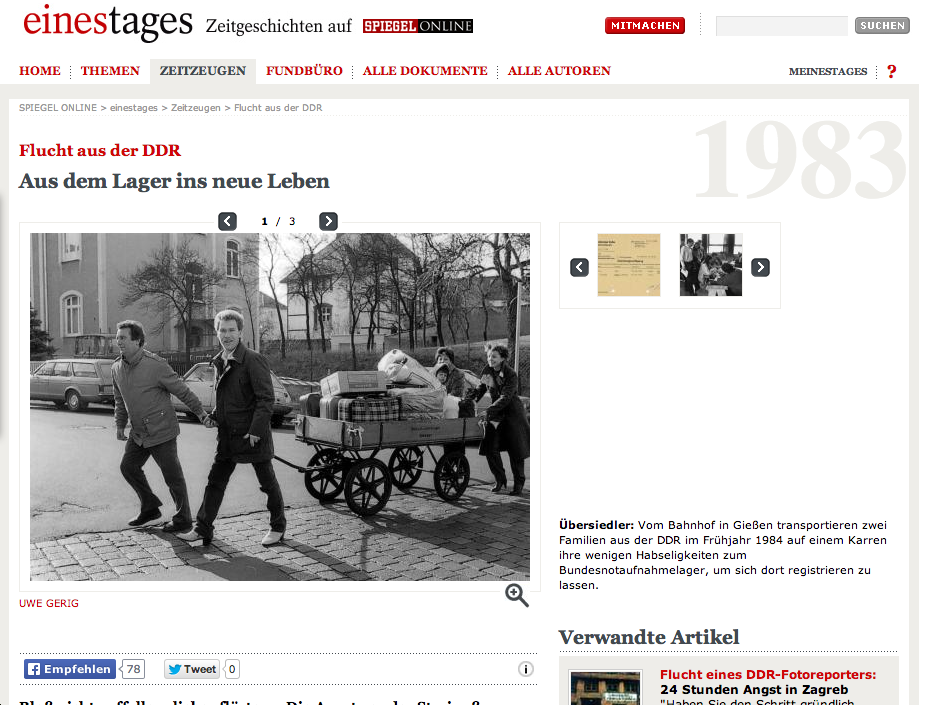
\includegraphics[width=1\textwidth]{einestages.png}
		\caption{einestages - Webseite}
	\end{center}
	\label{fig:einestages}
\end{figure}

\subsection{Google Music Timeline}
Zu nennen ist au�erdem die Google Music Timeline \citep{googleMusicTimeline}, die \glqq die Entwicklung der Musik-Genres seit 1950\grqq \ visualisiert \citep{googleMusicTimelineHeise}. W�hlt man eines der am Zeitstrahl visualisierten Musik-Genres, sieht man die Verteilung der jeweiligen Sub-Genres. Mit Klick auf eines der Sub-Genres, wird die Verteilung der Sub-Genre zugeh�rigen Interpreten angezeigt. Diese Verteilung wird aus den Statistiken von Google Play Music aggregiert und zeigt an, welche Interpreten und Alben die User in ihrer Musik-Bibliothek haben (\citeauthor[Vgl.][]{googleMusicTimelineAbout}). Auf der Abbildung \ref{fig:googleMusicTimeline} sieht man die Verteilung der Musik-Genres am Zeitstrahl. Darunter sieht man die popul�rsten Alben der gerade ausgew�hlten Genres, in diesem Fall wurde \glqq Rock\grqq \ ausgew�hlt.
\begin{figure}[htb]
	\begin{center}
		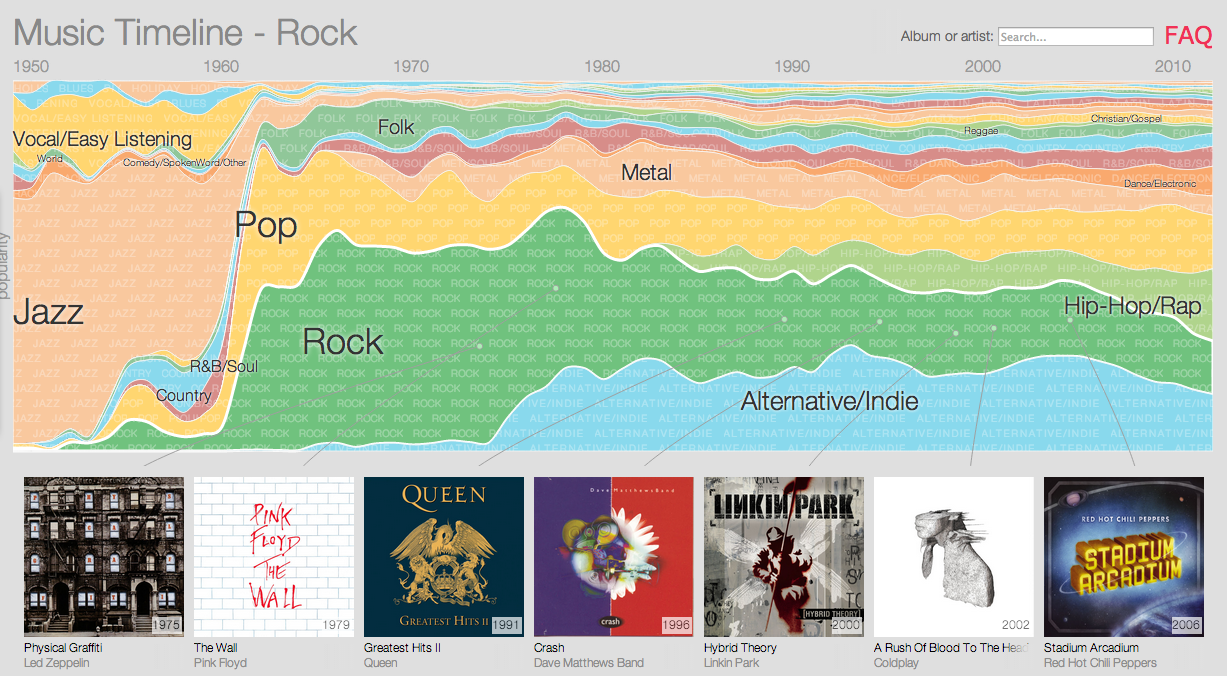
\includegraphics[width=1\textwidth]{googlemusictimeline.png}
		\caption{Google Music Timeline}
	\end{center}
	\label{fig:googleMusicTimeline}
\end{figure}


\subsection{Internet Archive - Wayback Machine}
Einen weiteren Ansatz bietet \textbf{Wayback Machine} \ \citep{wayback}. Auf der Startseite hei�t es, dass 386 Billion Websites im Laufe der Zeit gesichert wurden \citep[Vgl.][]{wayback}. Somit k�nnen alte Versionen der in der Suche registrierten Wesites besucht werden. Daf�r wird entweder eine Website aus dem Repertoire ausgesucht oder es wird nach der gew�nschten Website gesucht. Anhand eines Zeitstrahles kann dann in der Geschichte der Website gest�bert werden und die einzelnen Versionen der Website besucht werden. Auf der Abbildung \ref{fig:wayback} sieht man als Beispiel einen Screenshot der Website Yahoo.com, die das Internet Archive am 2.Mai 2005 gemacht hat. �ber dem Screenshot selbst ist ein Zeitstrahl zu sehen, der zur Navigation durch die verschiedenen Screenshots aus der Vergangenheit dient.
\begin{figure}[htb]
	\begin{center}
		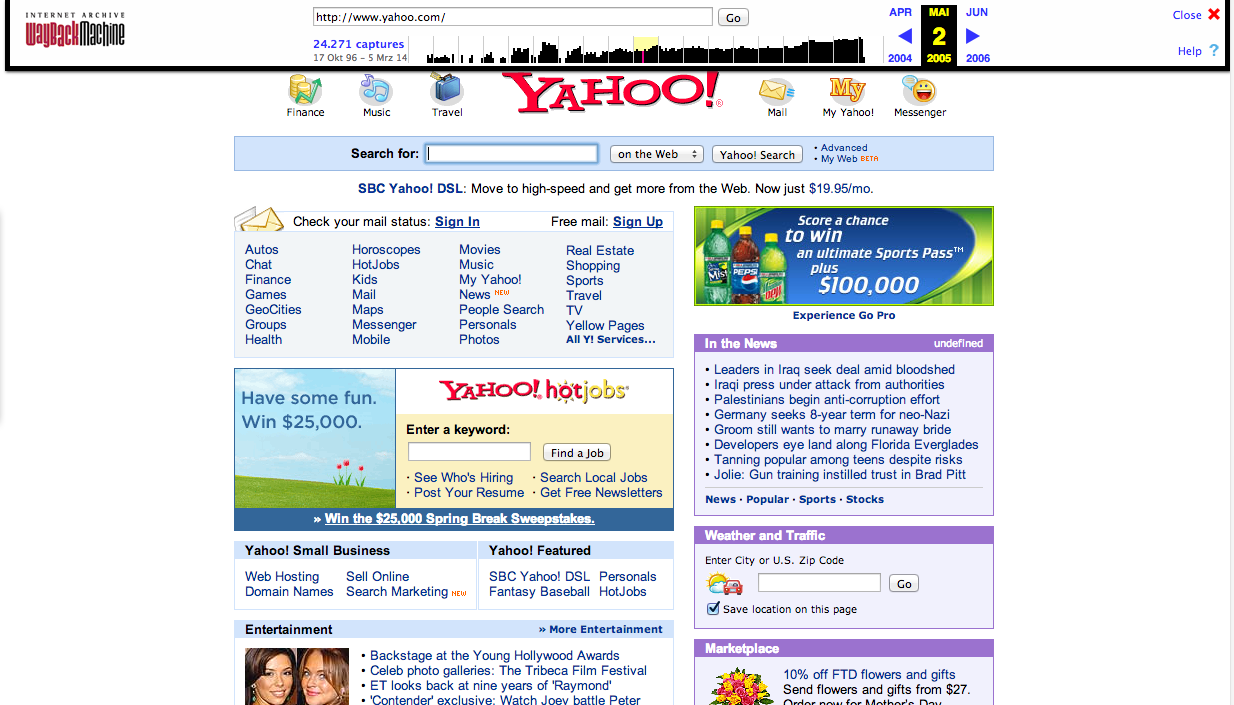
\includegraphics[width=1\textwidth]{wayback_yahoo.png}
		\caption{Internet Archive : Wayback Machine}
	\end{center}
	\label{fig:wayback}
\end{figure}



\chapter{Grundlagen}
\label{cha:grundlagen}
Im Folgenden werden f�r diese Arbeit wichtige grundlegende Begriffe gekl�rt, die im Laufe dieser Arbeit vorrausgesetzt werden.
% Darauf aufbauend kann der Anforderungsumfang gekl�rt werden.

%===================%
%===== SECTION =====%
%===================%
\section{Definitionen}
Nach \citeauthor{Misoch2006} werden Medien in vier unterschiedliche Typen differenziert. Prim�re Medien, Sekund�re Medien, Terti�re Medien und Quarti�re Medien. Hier werden die Medienformen nach Bedarf von Hilfsmittel kategorisiert, sodass \zB Gestik und Mimik unter Prim�re Medien zu fassen sind, Bild, Buch und Druck zu Sekund�ren Medien zu z�hlen sind. Terti�re Medien bed�rfen \glqq sowohl auf Produzenten- als auch auf der Rezipientenseite technische Hilfsmittel\grqq (\citefield[Seite 20]{shortauthor}{Fassler1997}), \ua Schallplatten, Film, Fensehen und Radio. Dar�berhinaus sind vernetzte Computermedien als Quarti�re Medien zu verstehen. 

\paragraph{Medium}
\label{par:medium}
Hypermedien werden von \citeauthor{Misoch2006} als Medienformen bezeichnet, die aufgrund der Entstehung digitaler Datenformate mit modernen Medientypen kombiniert werden. \Dahe \glqq Text, Bild, Sound usw. k�nnen miteinander verbunden werden\grqq \ (\citefield[Vgl. Seite 21]{shortauthor}{Misoch2006}).

Im Allgemeinen werden in dieser Arbeit haupts�chlich die Medienformen, die von \citeauthor{Fassler1997} anhand der Eigenschaft, dass Sender und Empf�nger jeweils �ber \glqq die computerbasierten und -verst�rkten Medienbereiche netztechnischer und elektronisch-r�umlicher Konsumption, Information und Kommunikation\grqq \ verf�gen m�ssen, eingeordnet (\citefield[Vgl. Seite 117]{shortauthor}{Fassler1997}).

Im Laufe dieser Arbeit sind unter dem Begriff der \textbf{Medien} die \textbf{Hypermedien} zu verstehen, die im Folgenden in Audio, Video, Text \usw kategorisiert werden.

\paragraph{Medientyp}
\label{par:medientyp}
�ber die vorangeganene Definition des Mediums hinaus, ist der im Laufe dieser Arbeit verwendete Begriff \textbf{Medientyp} als Unterscheidung zwischen den Medienformen Audio, Video, Text \usw zu verstehen.

\paragraph{Medienart}
\label{par:medienart}
Zur weiteren Gliederung von Medientypen, werden \textbf{Medienarten} im weiteren Verlauf daf�r verwendet, Sub-Medien zu unterscheiden. Bei den Medienarten des Medientyps Audio wird \bspw zwischen Musik, H�rspielen oder Radiosendungen unterschieden, w�hrend der Medientyp Video in Film, Reportagen, Video-Spiele \etc unterteilt werden kann.

\paragraph{Medien-Item}
\label{par:item}
Ist die Rede von einem Medien-Item, ist damit das einzelne Objekt eines Medientyps gemeint. \Bspw ein Musikst�ck, ein Musikalbum, ein News-Artikel, ein Film, eine TV-Serie, etc. Es wird \zB nach Medien-Items unterschiedlicher Medienarten und -typen gesucht, besteht das Ergebnis \bspw aus Medien-Items der Medienarten Musik und Film, wenn nur diese aufgelistet werden. Insbesondere wird auch ein Datum als Item bezeichnet, sollte es das Ergebnis einer Suche sein.

\paragraph{Dienst}
\label{par:dienst}
Im weiteren Verlauf wird von Diensten, Internet- und Suchdiensten gesprochen. Hier sind die unterschiedlichen Angebote des Internets im Sinne von Website-Diensten zu verstehen. \ZB werden Wikipedia.org, Google.de \etc jeweils als Suchdienste bezeichnet, auch wenn Wikipedia genauer auch als Nachschlagewerk zu betrachten ist. Das Gleiche gilt f�r Musikdienste wie \zB last.fm, Spotify oder MusicBrainz, die im Folgenden sowohl als Dienst, als auch spezifischer als Musikdienste betitelt werden.

\paragraph{Zeitpunkt}
\label{par:zeitpunkt}
In dieser Arbeit wird von Zeitpunkt gesprochen, sobald sich ein spezifisches Datum anhand eines Items ableiten l�sst. Bei der zeitspezifischen Recherche, wird bei einer Suche nach einem Zeitpunkt jedoch der unmittelbare Zeitraum, der den Zeitpunkt beinhaltet betrachtet.

\paragraph{Zeitraum}
\label{par:zeitraum}
Es wird ausdr�cklich von Zeitraum gesprochen, wird dieser durch die Suche des Nutzers oder anhand eines Items, das einen Zeitraum beschreibt, definiert. Insbesondere sind es Zeitr�ume, die gr��ere Zeitspannen mehrerer Jahre beinhalten.

%===================%
%===== SECTION =====%
%===================%
\chapter{Analyse}
Nachdem untersucht wurde, welche L�sungen und Ans�tze es im Internet bereits gibt, um Informationen gezielt aus der Vergangenheit zu durchsuchen, stellt sich die Frage, welche M�glichkeiten im Internet existieren, \bzw Schritte n�tig sind, um Daten eines spezifischen Zeitraumes verschiedener Medientypen zu aggegieren.

\section{Herangehensweise eines Nutzers und Evaluierung potenzieller Datenquellen}
\label{sec:analyse}
% Gegen�berstellung von Herangehensweise eines Nutzers und Evaluierung potenzieller Datenquellen

%Bitte besser beschreiben, dass es sich bei Google um eine Breitensuche handelt (und daher ja auch erst das medium wie "movies" mitangegeben werden muss). Versus die "direkte" suche bei Portalen die auf das gesuchte Medium beschr�nkt sind
Das Ziel der Web-Applikation ist es, zeitabh�ngige Daten zu liefern. Das bedeutet, dass je nach Vorgabe eines Zeitraumes, \bzw eines Zeitpunktes, Medien-Inhalte aus dem Internet, die dem vorgegebenen Zeitraum zuzuordnen sind, angezeigt werden sollen. Im Folgenden wird analysiert, welche Daten auf welche Art und Weise im Internet zu finden sind und inwiefern ein Nutzer heutzutage vorgehen m�sste, um zeitspezifisch nach Medieninhalten zu suchen.

Um einen besseren Vergleich der vorhandenen Suchdienste zu bekommen, wird zun�chst die Vorgehensweise eines Nutzers, der nach Inhalten verschiedenen Typs innerhalb eines selbst gew�hlten Zeitraumes sucht, erl�utert. Dabei werden auch m�gliche Dienste, die dieser nutzen k�nnte, kurz vorgestellt. 

Der Vorgehensweise des Nutzers wird eine Evaluation der potenziell in Frage kommenden Suchdienste und APIs f�r die jeweiligen Medientypen gegen�bergestellt, indem diese anhand �hnlicher Suchbegriffe miteinander verglichen werden. Das wichtigste Kriterium der Auswahl der Suchdienste ist, ob der gew�nschte \bzw erwartete Kontent auf der Website vorhanden ist \bzw den Kontent liefern k�nnen. \ZB werden Musikinhalte nicht in Filmdatenbanken gesucht, gleichzeitig wird Google mit einbezogen, da es ebenfalls Film-, Musik- und Video-Ergebnisse liefern kann. Au�erdem muss bei speziellen Medienplattformen die M�glichkeit bestehen, die Website nach Inhalten zu durchsuchen. Auch spielt die Popularit�t der Suchmachine \bzw Website eine Rolle, da dies tendenziell ein positiver Anhaltspunkt f�r die Plausibilit�t der vorhandenen Daten und der Funktionalit�t der Suche ist.

Dabei gilt es die Funktionsweise der Breitensuche, wie Google diese durchf�hrt, von einer direkten Suche zu unterscheiden. Das bedeutet, dass bei einer Google-Suche mit angegeben werden muss, welches Medium gesucht wird. Zum einen weil Google auch eine Bild- und Video-Suche beinhaltet und damit bereits gezielt nach diesen Medientypen gesucht werden kann, zum anderen, weil bei einer Google-Suche \bspw der Begriff \textbf{90s} allein keine Aussage dar�ber enth�lt, dass Musik aus dieser Zeit gesucht wird, w�hrend das bei Diensten wie last.fm oder IMDb aufgrund des Angebots direkte Vorraussetzung ist.

%Der grobe Ablauf, der in den Schemata zu sehen ist, l�sst sich somit in zwei Schritte trennen. Zun�chst wird die Eingabe des Nutzers, sei es ein Datum oder ein Item, aus dem sich ein Datum extrahieren l�sst, in einen Zeitraum �bersetzt, es sei denn, es wird ein Zeitraum eingegeben.

%Der zweite Schritt besteht daraus, passende Inhalte aus dem Zeitraum zu sammeln und anzuzeigen.

Um f�r die Suche m�glichst einfache Parameter zu w�hlen, wird die Suche au�erdem in englisch durchgef�hrt und m�glichst einfache Rahmenbedingungen geschaffen. Die Funktion der erweiterten Suche wird \ggf seperat betrachtet.

Es wurde nach den Begriffen \textbf{80s}, \textbf{90s} und \textbf{vietnam war} gesucht, w�hrend jeder dieser Begriffe einen Zeitraum repr�sentiert. Die Wahl von zwei Jahrzehnten dient dazu, einen besseren Vergleich ziehen zu k�nnen, ob �hnliche Suchanforderungen auch ebenso �hnliche Suchergebnisse liefern, \zB ob der erste Suchbegriff bei Google immer ein Ergebnis von dem Musikdienst lastfm.de liefert. 

Im Bereich Musik wird zus�tzlich nach \textbf{David Bowie - Changes} gesucht, da dies ein m�glicher Begriff ist, den die entwickelte Web-Applikation bedienen soll. Die Suchbegriffe wurden ggf. an den Suchdienst angepasst, \zB in der Amazon-Suche zu sehen, wo jeweils die passenden Filter (Music, Movies \& TV) gew�hlt wurden und die Begriffe \glqq music\grqq \ und \glqq video\grqq \ daf�r ausgelassen wurden. Bilder- und Video-Ergebnisse bei Google werden ausgelassen, mit Ausnahme der Suche nach Kunst in einem bestimmten Zeitraum. Hier wird lediglich die Bildersuche in Betracht gezogen.

Das Ergebnis der Evaluierung wird anhand einer Matrix dargestellt, in denen die Bereiche Musik, Film, Kunst und Ereignisse betrachtet werden. In jeder Matrix sind die Ergebnisse nach Suchdiensten sortiert. Es werden jeweils die ersten drei Suchergebnisse aufgelistet, zusammen mit dem Titel des Beitrages (�berschrift auf der Seite, Titel des thematisierten Items, etc.). Darauf folgt eine kurze Beschreibung des Inhalts, der schnellen Aufschluss �ber die Relevanz der gefundenen Ergebnisse liefert.

%\subsection{Bewertung der Suchergebnisse}
Zur Bewertung des Suchergebnisses werden verschiedene Aspekte betrachtet: thematische Relevanz, Qualit�t des Suchergebnisses, gemessen an der Herkunft, Glaubw�rdigkeit und Objektivit�t der Daten. Das bedeutet, dass lediglich die Komfortabilit�t der Suche und die Relevanz und Auswertbarkeit der Ergebnisse untersucht wird.

\subsection{Herangehensweise eines Nutzers im Bereich Musik}
Zur dynamischen Zusammenstellung von Musik, insbesondere einer gew�nschten Zeit, gibt es derzeit eine Vielzahl von M�glichkeiten. Gute Ergebnisse bieten manuell erstellte Playlisten, Musik-Sampler oder CD-Sammlungen. Jedoch sind diese Inhalte entweder nicht dynamisch oder leiden an der M�glichkeit der Spezifizierung.
Im Internet gibt es unz�hlbar viele Dienste, die es dem Nutzer erm�glichen unterschiedlichste Zusammenstellungen von Musiktiteln zu h�ren. Dazu geh�ren \zB �ffentlich verf�gbare Playlisten und Streaming-Dienste. Diese und weitere derzeit verf�gbare M�glichkeiten Musik einer gew�nschten Zeit zu h�ren, werden im Folgenden kurz vorgestellt.

\paragraph{Themenorientierte Radiosendung/Spezielle Radiosender}
Eine der g�ngigsten Methoden ist es, einen Radiosender, der vorwiegend Musik des gew�nschten Zeitraums spielt. So gibt es zahlreiche Radiosender und -shows, die sich auf Musik aus den 80er oder 90er Jahren spezialisiert haben. Zum Beispiel sind die Online-Streaming-Angebote von \textbf{SAW Musikwelt} \citep{sawMusikwelt}, wo f�r die Jahrzehnte 70er, 80er und 90er jeweils ein Radiosender angeboten wird, und  \textbf{FFH Webradio} \citep{ffhRadio}. Dies erm�glicht zwar eine meist zuverl�ssige Eingrenzung f�r einen bestimmten Zeitraum, jedoch gibt es in dieser Form kein Angebot, das sich auf einen genaueren Zeitraum beschr�nkt. Zwar gibt es \ua spezielle Shows, die Musik eines genaueren Zeitraums spielen (\bspw eine Radioshow, die sich konkret mit einem bestimmten Jahr befasst), doch sind diese meist zeitlich begrenzt und nicht auf Anfrage abrufbar.

\paragraph{Online-Streaming anhand eines Tags}
Bei zahlreichen Online-Streaming-Diensten kann der Nutzer Musiksender anhand eines Tags erstellen lassen. Diese Funktionalit�t bietet \bspw \textbf{Last.fm} \citep{lastfm} an. Dies k�nnen \zB Tags wie \glqq 1970\grqq, \glqq 70er\grqq, \glqq seventies\grqq, \glqq siebziger\grqq \ oder \glqq 70\grqq \ sein. Diese Tags werden jedoch meist von Usern dieser Plattformen gepflegt, \dahe dass diese unvollst�ndig oder fehlerhaft sein k�nnen. Au�erdem sieht man bereits daran, dass Tags, die im Grunde das gleiche bedeuten, aber verschieden buchstabiert werden, wie komplett unterschiedliche Tags behandelt werden. So ist die Band Spice Girls bei last.fm \uU mit den Tags \glqq girl band\grqq, \glqq girl bands\grqq, \glqq girl group\grqq, \glqq girl groups\grqq, \glqq girl power\grqq, \glqq girlband\grqq, \glqq girlbands\grqq \ und \glqq girls group\grqq \ versehen, woran deutlich zu erkennen, dass diese Tags semantisch die gleiche oder zumindest eine �hnliche Bedeutung haben. Um diese Missverst�ndnisse zu umgehen, gibt es bei last.fm zus�tlich die M�glichkeit Web-Radio nach einem \textbf{Global Tag} \citep{lastfm80s} zu h�ren. Sich jedoch dar�ber hinaus Musik eines bestimmten Jahres anhand eines Tags anzuh�ren ist zu einem nicht gegeben \bzw unzuverl�ssig, sollte das Tag falsch gepflegt worden sein.

%====

\subsection{Evaluierung der Suchdienste im Bereich Musik}
Im Bereich Musik hat die Suche insgesamt die am besten passenden Ergebnisse geliefert. Das bedeutet, dass sich die gefundenen Ergebnisse gr��tenteils auf Musik beziehen und thematisch auch das Gesuchte wiederspiegeln.
Die im Bereich Musik untersuchten Dienste sind in der Tabelle \ref{tab:musicSearches}, nach Suchtyp geordnet, aufgelistet.

\begin{table}[H]
	\begin{center}
		\begin{tabular}{|c||c c c|}
		  %Medientyp & bla & bla \\ \hline\hline
		  \hline
		  Suchtyp & & Suchdienst & \\ \hline\hline
		  Breitensuche & google.de & en.wikipedia.org & amazon.com \\ \hline
		  Spezifische Suche & last.fm & Spotify App & \\ \hline
		\end{tabular}
		\caption{Untersuchte Suchdienste im Bereich Musik}\label{tab:musicSearches}
	\end{center}
\end{table}

Dabei hat Google meist auf Ergebnisse der anderen analysierten Suchdienste verwiesen, \zB auf lastfm.de mit \glqq 80s\grqq \ getaggte Musik. Auff�llig ist hier, dass die von Google gefundenen Ergebnisse, die auf andere untersuchte Suchdienste verweisen, in einigen F�llen passendere Ergebnisse liefern, als das Suchen auf der spezialisierten Seite selbst. Als Beispiel sei zum einen die Suche in der Kategorie Musik mit dem Suchbegriff \glqq music vietnam war\grqq \ genannt. Hier liefert Google als erstes Suchergebnis den Wikipedia-Artikel \glqq List of songs about the Vietnam War\grqq \ \citep{wikiListSongsVietnamWar}, w�hrend dieser Artikel in der Wikipedia-Suche mit dem selben Suchbegriff gar nicht auftaucht, gleichzeitig aber auch keine besseren Ergebnisse liefert. Jedoch befinden sich in den Suchergebnissen auch subjektive Musik-Charts, die Privatpersonen nach eigenen Kriterien erstellt und online gestellt haben.

Verh�ltnism��ig gute Ergebnisse liefert auch amazon.de mit Kompilationen und CD-Sammlungen aus den Jahrzehnten und der Zeit des Vietnamkrieges. Zwar befindet sich in den aufgef�hrten Suchergebnissen ausschlie�lich Musik, die direkten Bezug zum Vietnamkrieg hat, jedoch ist die amazon-Suche nicht darauf ausgelegt, semantisch passend zum Begriff zu suchen.

Die Suche der Musik-Datenbank \textbf{RateYourMusic} \citep{rymHome} bietet unter \textbf{Charts} eine Suche an, die die Erstellung einer Chart-Liste nach selbst gew�hlten Kriterien zul�sst. Es ist eine Erstellung von Chartlisten pro Jahr ab 1900 m�glich. Alternativ k�nnen Chart-Listen der Jahrzehnte des 20. und 21. Jahrhundert erstellt werden. Zus�tzlich kann die Chartliste nach Genre eingegrenzt werden. Dementsprechend k�nnen die Ergebnisse f�r die Jahrzehnte \glqq 80s\grqq \ und \glqq 90s\grqq \ von RateYourMusic als sehr gut bewertet werden. Nachteil der vorgegebenen Jahre und Jahrzehnte ist, dass es �ber das Frontend nicht m�glich ist, Charts aus selbst gew�hlten Zeitr�umen zu erstellen. 

Daf�r, dass die Online-Musik-Datenbank Musicbrainz ein gro�es Repertoire an Musik-Ver�ffentlichungen hat, dessen Werte zumindest f�r einen Gro�teil popul�rer Ver�ffentlichungen ausf�hrlich gepflegt sind, gibt es keine M�glichkeit, auf Musicbrainz.org zeitspezifisch zu suchen.

\subsection{Herangehensweise eines Nutzers im Bereich Film}
Eine Zusammenstellung von Filmen, die sich einem gew�hlten Zeitpunkt zuordnen lassen, sind meistens finite Listen, die von Privatpersonen, Filmorganisationen \oae zusammengestellt werden oder Filmsammlungen, die \zB die popul�rsten Filme einer Epoche, eines Jahrzehnts oder eines Themas enthalten. Listen verschiedenster Kriterien sind zahlreich im Internet zu finden, jedoch sind diese oft nicht dynamisch, sondern setzen vorraus, dass sich vorher eine Person mit dem Thema auseinandergesetzt hat. Ansonsten bleibt nur das manuelle Erstellen solch einer Liste.

\paragraph{Suche nach Filmen �ber Amazon}
Der Online-Versandhandel Amazon.com bietet \ua eine gro�e Auswahl an Filmen im Sortiment. Die erweiterte Suche l�sst auch die gezielte Suche nach Titeln der Kategorie \glqq Movies \& TV\grqq \ und ein Filtern nach Jahrzehnt zu. Genauer l�sst sich der Zeitraum nicht eingrenzen, au�erdem beschr�nken sich die Suchergebnisse auf Produkte, die Amazon.com anbieten kann.

\paragraph{Suche nach Filmen �ber IMDb}
Die Internet Movie Database IMDb.com ist die bekannteste und autorit�rste Quelle f�r Film, TV und Prominente der Filmbranche \citep[Vgl.][]{imdbPress}. IMDb.com umfasst neben detaillierten Informationen �ber einzelne Kino-, Video- und Fernseh-Produktionen auch Informationen �ber Videospiele \citep{imdbStats}. IMDb bietet hier derzeit die zuverl�ssigste M�glichkeit, Filme aus einem begrenzten Zeitraum nach Kriterien wie dem MOVIEMeter oder User Rating zu sortieren.

\subsection{Evaluierung der Suchdienste im Bereich Film}
Auch im Bereich Film variiert die Qualit�t und Relevanz der Suchergebnisse stark zwischen den unterschiedlichen Suchdiensten. Folgende Dienste sind analysiert worden:Die untersuchten Dienste im Bereich Film sind in der Tabelle \ref{tab:movieSearches} nach Suchtyp aufgelistet.

\begin{table}[H]
	\begin{center}
		\begin{tabular}{|c||c c c|}
		  %Medientyp & bla & bla \\ \hline\hline
		  \hline
		  Suchtyp & & Suchdienst & \\ \hline\hline
		  Breitensuche & google.de & en.wikipedia.org & amazon.com \\ \hline
		  Spezifische Suche & IMDb & & \\ \hline
		\end{tabular}
		\caption{Untersuchte Suchdienste im Bereich Film}\label{tab:movieSearches}
	\end{center}
\end{table}


Die ersten Ergebnisse der Google-Suche nach \glqq movies 80s\grqq \ und \glqq movies 90s\grqq \ belaufen sich gr��tenteils auf h�ndisch erstellte Listen von Privatpersonen. Unter den Ergebnissen befinden sich jedoch auch Verweise auf zwei Wikipedia-Artikel, die jeweils die popul�rsten Filme der Achtziger und Neunziger auflisten. W�hrend Google \ua auf diese Wikipedia-Artikel verweist, ist das Ergebnis der Suche nach dem entsprechenden Begriff auf Wikipedia selbst weniger erfolgreich. Hier taucht nur einer der sehr gut passenden Wikipedia-Artikel auf. Stattdessen werden Artikel gefunden, die gr��tenteils nichts mit dem Thema Film zu tun haben, sondern sich \zB mit Musik oder Pers�nlichkeiten besch�ftigen, was darauf zur�ckzuf�hren ist, dass die Wikipedia-Suche textuell sucht. Im Gegensatz dazu, liefert die Wikipedia-Suche nach Filmen w�hrend des Vietnamkrieges �u�erst relevante Ergebnisse.

Amazon.com liefert mit Zuhilfenahme des Filters \glqq Movies \& TV\grqq \ haupts�chlich Filmsammlungen, die in Anbetracht des Suchbegriffes passend sind, was auch auf die Suche nach Filmen aus dem Vietnamkrieg zutrifft.

Eine Standardsuche nach den entsprechenden Suchbegriffen auf IMDb.com verdeutlicht, dass es sich um eine Titelsuche handelt. Erst eine erweiterte Suche mit den eingestellten Parametern des jeweiligen Zeitraumes resultiert in eine Liste von ausschlie�lich zeitlich passenden Eintr�gen. Dabei gilt, dass der Zeitraum des Vietnamkrieges anhand von Daten eingegeben werden muss und nicht nach dem Begriff selbst gesucht werden kann. 


\subsection{Herangehensweise eines Nutzers im Bereich geschichtlicher Ereignisse}
Eine zeitspezifische Suche nach geschichtlichen Ereignissen \bzw News-Artikeln gestaltet sich weitaus schwieriger. Zwar gibt es im Internet zahlreiche Quellen an Informationen, jedoch sind diese oft nur hinl�nglich zeitabh�ngig auffindbar.

\paragraph{Geschichtliche Ereignisse}
Eine Suche nach geschichtlichen Ereignissen wird derzeit am besten von Wikipedia bedient. Zwar gibt es auch Geschichts-Datenbanken, jedoch sind diese bei weitem nicht so umfangreich und ausf�hrlich wie das Online-Lexikon Wikipedia. Ein Nachteil ist hier wiederrum, dass die Artikel auf Wikipedia nicht allein auf geschichtliche Ereignisse begrenzt sind. Weiterhin ist die Wikipedia-Suche nicht darauf ausgelegt, Ereignisse nach Datum zu finden. Zwar gibt es f�r zahlreiche Daten, wie \bspw den 11. November oder den 9. Januar, jeweils einzelne Artikelseiten mit einer Auflistung pr�gnanter Ereignisse dieses Datums, jedoch l�sst sich nicht nach einem Datum mit Jahr suchen. Ausnahme sind hier lediglich Daten mit eigenem Artikel, so leitet \zB die Suchanfrage \glqq 11. September 2001\grqq \ zum Artikel der \glqq Terroranschl�ge am 11. September 2001\grqq \ \citep{wikiTerror}.

\paragraph{News}
Zeitungsartikel weisen eine weitere Schwierigkeit auf. Die ersten Internetauftritte gab es in den 90er Jahren, dementsprechend gibt es bei Zeitungsartikel aus weiter vorangegangener Zeit eine weitaus geringere Dichte, wenn �berhaupt. So gibt es mittlerweile viele Internet-Zeitungen und -Magazine, die ihre Archive online zur Verf�gung stellen, teiweise auch kostenlos. Dazu geh�ren im deutschsprachigen Raum \ua ZEIT ONLINE \citep{zeitArchiv}, die S�ddeutsche Zeitung \citep{szArchiv}, die Frankfurter Allgemeine Zeitung \citep{fazArchiv} und der Spiegel \citep{spiegelArchiv}. Eine �bergreifende Suche in den Zeitungs-Archiven gibt es bisher nicht.


\subsection{Evaluierung der Suchdienste im Bereich geschichtlicher Ereignisse}
Die Suche nach Ereignissen f�hrt auf Google neben einem Wikipedia-Artikel der \glqq Zusammenfassung der wichtigsten Ereignisse der 80er\grqq \ auf einen Artikel des Bildungsdienstes about.com, der eine Auswahl an wichtigen Ereignissen der 80er-Jahre auff�hrt, und auf eine eher verspielte Webseite einer Privatperson, die sich ebenfalls mit den 80er-Jahren besch�ftigt. Die Suche nach \glqq vietnam war\grqq \ auf Google hat die zufriedenstellendsten Ergebnisse, \va im Aspekt der Glaubw�rdigkeit der Webseiten. 

Wikipedias Ergebnisse zu Ereignissen der verschiedenen Zeitr�ume f�llt im Falle des Vietnamkrieges am besten aus, w�hrend die anderen Epochen gr��tenteils auf Wikipedia-Artikel von Sportvereinen f�hren. 

Hier liefert history.orb gr��tenteils passende Ergebnisse, bietet \ua aber auch Ergebnisse anderer Zeitperioden. Wolfram Alpha scheint die Suchanfrage einer Epoche nicht interpretieren zu k�nnen und liefert stattdessen Wortbedeutungen, obwohl eine Suche nach einem bestimmten Ereignis alle n�tigen Informationen enth�lt, die es ben�tigt, eine Auflistung passender Ereignisse nach Datum zu liefern.

\subsection{Herangehensweise eines Nutzers im Bereich Bild und Bildende Kunst}
Im Bereich Bild und Kunst gestaltet sich eine zeitspezifische Suche weitaus schwieriger. Zwar l�sst sich ein Gro�teil allgemeiner Informationen und Meta-Daten �ber Kunstwerke und Gem�lde im Internet finden, eine umfassende Suche gibt es jedoch nicht. Spezielle Suchmaschinen durchsuchen \bspw einen begrenzten Katalog, \bspw die Sammlung eines bestimmten Kunst-Archivs und sind zudem oft veraltet und teilweise unvollst�ndig. 

\paragraph{Kunst-Archive im Internet}
So enth�lt \bspw das Art Archive �ber eine Bilder-Bibliothek aus �ber 900 Quellen weltweit, wobei der Entstehungszeitraum vom 30. Jahrhundert v. Chr. bis ins 20. Jahrhundert reicht \citep[Vgl.][]{artArchive}. Dies ist zwar eine umfangreiche Sammlung, jedoch gibt es auch nicht zu jedem Datensatz ein Bild aufgrund von Copyrights. Au�erdem ist die Suche eher darauf ausgelegt nach K�nstlernamen \oae zu suchen, die man nach Themengebiet filtern kann, als auf einen bestimmten Zeitraum.

�ber die Suchmaschine der Web Gallery Of Art \citep{webGalleryOfArt} l�sst sich die Suche in F�nfzig-Jahr-Schritten, auch ohne Eingabe eines Suchbegriffs, eingrenzen. Daf�r sind in der Datenbank lediglich Kunstwerke bis einschlie�lich 1900 zu finden.

Dar�ber hinaus gibt es noch weitere M�glichkeiten nach Kunstwerken zu suchen, jedoch sind diese meist auf den Verkauf von Kunst ausgelegt, das bedeutet, dass auch nur die Kunstwerke in der Datenbank gefunden werden k�nnen, die durch den Service auch verkauft werden k�nnen. Ein Beispiel ist der Dienst The Art Online Gallery \citep{artOnlineGallery}.

Im Bereich Kunst ist die Abh�ngigkeit von der Art der Implementierung der Suche besonders gro�. So hat man oft lediglich die M�glichkeit aus einer begrenzten Anzahl an vorgegebenen Epochen auszusuchen.

Zus�tzlich lassen sich Bilder im Gegensatz zu Musik schwieriger finden, da es hier an Standards wie ID3 fehlt. Hier w�re eine allgemeine Suchfunktion, die sich auf Kunstwerke aller Art spezialisiert w�nschenswert. Bisher ist man hier auf existierende Kunstarchive angewiesen.


\subsection{Evaluierung der Suchdienste im Bereich Bildende Kunst}
Zwar gibt es im Bereich Bildender Kunst einige Suchdienste, jedoch sind diese f�r die Evaluation mit den gew�hlten Vorgaben nicht geeignet. Das Art Archive gibt \bspw Suchergebnisse wieder, die die Suchbegriffe \glqq 80s\grqq \ und \glqq 90s\grqq \ im Dateinamen enthalten. Die Web Gallery Of Art l�sst zwar das Filtern nach einer w�hlbaren Zeitspanne in ihrer Suche zu, jedoch sind die gew�hlten Zeitr�ume dieser Evaluierung nicht Teil der Datenbank. Die Suche der Art Online Gallery durchsucht lediglich gesetzte Tags und findet dementsprechend nur bei einer Suche nach \glqq vietnam war\grqq \ verschiedene Gem�lde, die auf der Seite k�uflich zu erwerben sind. Art Cyclopedia \citep{artCyclopedia} findet bei keinem der Suchbegriffe ein Ergebnis.


\subsection{Extrahierung eines Zeitpunktes}
In der vorangegangenen Analyse wird vorausgesetzt, dass der Nutzer bereits wei�, welchen Zeitraum er durchsuchen will. Dies funktioniert f�r weit gefasste Begriffe, die bereits einen Zeitraum beschreiben (Achtziger, Neunziger, etc.), weil diese auch als eine Art Epoche, die ihren eigenen Stil hervorgebracht haben, betrachtet werden k�nnen. 

W�hrend der Term \glqq Vietnam War\grqq \ \ua einen begrenzten Zeitraum beschreibt, funktioniert eine Suche nach zeitspezifischen Inhalten in diesem Fall au�erdem besser, weil Musik und Film auch direkt vom Vietnamkrieg beeinflusst wurden, indem das Thema in diesen Bereichen aufgegriffen und behandelt wurde. Das bedeutet, dass bei einer Suche nach \glqq Vietnam War Music\grqq \ nicht grunds�tzlich auf den Zeitraum datierte Musik gefunden wird, sondern auch Inhalte, die sich im Nachhinein darauf beziehen.

Wiederrum anders verh�lt sich eine Suche im Internet, wenn \bspw Medieninhalte aus dem Zeitraum der Entwicklung der Relativit�tstheorie angezeigt werden sollen. Hier halten sich Kulturg�ter k�nstlerischer Natur (Musik, Film, Bildende Kunst, etc.), die sich wie im Falle des Vietnamkrieges auf ein historisches Thema beziehen, in Grenzen. In diesem Fall, muss also zun�chst der Zeitpunkt der Ver�ffentlichung der Relativit�tstheorie herausgefunden werden, worauf dieser Zeitraum in einem zweiten Schritt durchsucht wird.

Im Folgenden werden M�glichkeiten vorgestellt, Zeitpunkte oder Zeitr�ume von Medientypen oder Ereignissen herauszufinden.

\paragraph{Google.de}
Bei einer Vielzahl von Begriffen, bietet Google.de bereits passende vorgefertigte Antworten in Form des \textbf{QuickAnswers}-Kasten an. Eine Eingabe einer prominenten Person gibt \ua das Geburtsdatum und \ggf das Todesdatum aus. Eine Eingabe des Filmtitels \glqq World War Z\grqq \ zeigt neben anderen Kerninformationen auch das Erscheinungsjahr des Films. Dies funktioniert f�r bestimmte Themenbereiche zuverl�ssig, w�hrend die Eingabe eines Musiktitels derzeit keine \textbf{QuickAnswers}-Funktionalit�t bietet. Ebenso liefert \textbf{QuickAnswers} derzeit keine Antwort f�r die Eingabe von \bspw \glqq Vietnam War\grqq \ oder \glqq Second World War\grqq .

\begin{figure}[htb]
	\begin{center}
		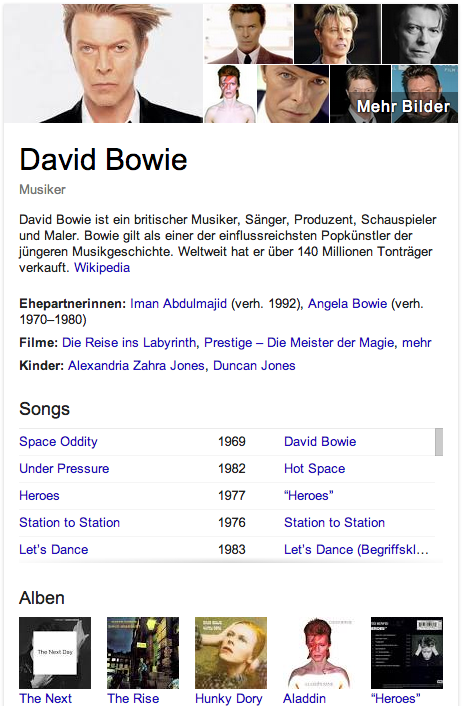
\includegraphics[width=0.49\textwidth]{quickAnswersBowie.png}
		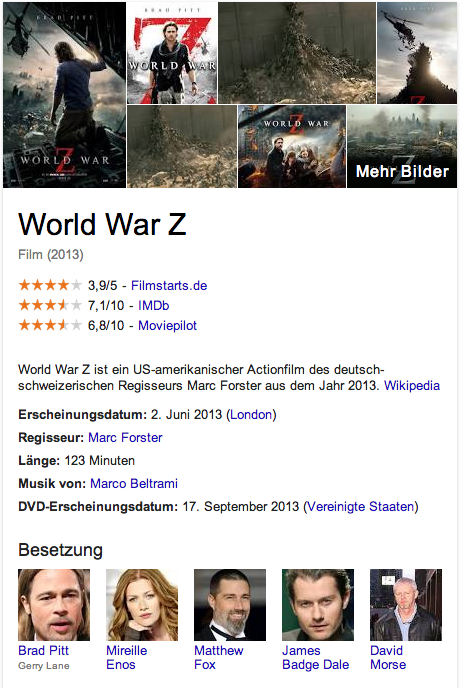
\includegraphics[width=0.49\textwidth]{quickAnswersWWZ.png}
		\caption{Beispiel der QuickAnswers-Box mit einer Eingabe von \glqq David Bowie\grqq (links) und \glqq World War Z\grqq (rechts)}
	\end{center}
	\label{fig:quickAnswers}
\end{figure}

\paragraph{Wolfram|Alpha}
Wolfram|Alpha bietet wie Google.de ebenfalls die M�glichkeit Suchbegriffe zu interpretieren und dementsprechend passende Informationen anzuzeigen. So werden die Begriffe \glqq�Vietnam War\grqq \ und \glqq�Second World War\grqq \ beide richtig als \glqq historical event\grqq \ interpretiert und ein Zeitraum in Form eines Zeitstrahles angegeben. Ebenso funktioniert das f�r die Eingabe von \glqq World War Z\grqq , der als \glqq movie\grqq interpretiert wird und neben anderen Informationen �ber den Film auch das Ver�ffentlichungsdatum ausgibt. Sogar die Eingabe von \glqq�this is the end doors\grqq \ gibt neben dem Songtext auch das Ver�ffentlichungsdatum aus. Allerdings ist diese Suche nicht immer zuverl�ssig, so besteht das Ergebnis der Eingabe von \glqq this is the end \textbf{the} doors\grqq \ aus dem Film \textbf{This is the end}.

\paragraph{Wikipedia}
Das Ergebnis bei einer Suche auf Wikipedia ist haupts�chlich davon abh�ngig, ob ein eingegebener Begriff richtig interpretiert wird. Gibt man in die Suche der englischsprachigen Wikipedia den Begriff \glqq vietnam war\grqq \ ein, gelangt man auf den Wikipedia-Artikel des Vietnam Krieges und sieht in der Box auf der rechten Seite die Datumsangaben des Krieges. Gleiches gilt f�r die Eingabe von \glqq second world war\grqq . Eine Eingabe von \glqq the doors the end\grqq \ f�hrt hingegen erst auf eine Suchergebnis-Seite statt direkt auf den passenden Artikel umzuleiten. Navigiert man auf den Wikipedia-Artikel des Songs, sind sowohl das Aufnahmedatum, als auch das Ver�ffentlichungs-Datum in der seperaten Box sichtbar.

\paragraph{Wikidata}
Sucht man auf Wikidata nach \glqq second world war\grqq \ wird man wie auf Wikipedia erst auf eine Suchergebnisseite umgeleitet, woraufhin man zu dem passenden Eintrag navigieren kann. Hier ist allerdings keine Zeitangabe zu finden. Eine Eingabe von \glqq david bowie changes\grqq \ leitet �ber den Umweg einer Suchergebnisseite ebenfalls auf den Eintrag des Songs. Auch hier ist keine Information �ber das Ver�ffentlichungsdatum zu finden. Wohingegen der Eintrag �ber \textbf{David Bowie} selbst zumindest das Geburtsdatum erschlie�en l�sst.

\paragraph{Zusammenfassung}
Es gibt bereits gute Ans�tze der untersuchten Dienste, Eingaben richtig zu interpretieren und einen passenden Satz an Informationen auszugeben. Im Falle von Google kommt es derzeit darauf an, welche Art von Suchbegriff eingegeben wird. F�r Filme und Personen liefert \textbf{QuickAnswers} gute Ergebnisse. Sowohl die geschichtlichen Zeitr�ume, als auch Musikver�ffentlichungen konnten dagegen nicht aufgel�st werden. Insbesondere Wolfram|Alpha bietet insgesamt gute Ergebnisse, die sich f�r eine Nutzung f�r die Entwicklung der Web-Applikation anbietet. Wikipedia verf�gt �ber ein riesiges Repertoire an Artikeln, hier ist der Erfolg der Suche aber davon abh�ngig, ob eine Eingabe von der Suche direkt in einen passenden Artikel �bersetzt werden kann, da ansonsten eine maschinelle Auswertung dementsprechend komplexer ist.

\subsection{Auswertung}
Allgemeines Problem insbesondere bei News-Artikeln ist die relationale Suche. Internetsuchmaschinen wie Google suchen prim�r relational, \dahe , dass das Suchen nach Inhalten, die lediglich zeitlich mit dem gesuchten Begriff zu tun haben, deutlich schwieriger \bzw seltener im Internet vorhanden ist. \citeauthor{Heuser2011} formuliert diese Tatsache wie folgt: 
\begin{quotation}\glqq Semantische Technologien bieten zahlreiche M�glichkeiten, um Daten mit Hintergrundinformationen zu ihrer Bedeutung anzureichern und sie mit weiteren relevanten Informationseinheiten zu verbinden.\grqq \newline \citeauthor[Vgl. Seite 19,][]{Heuser2011}\end{quotation}
Das verdeutlicht, inwiefern semantische Suchen der Implementierung der Web-Anwendung dienlich sein k�nnten, wobei im Gegensatz dazu aus der Evaluation der Suchmaschinen hervorgeht, dass diese noch nicht implementiert sind, \bzw noch nicht ausgereift sind.

%Hier fehlt komplette die Auswertung �ber die Qualit�t der Suchergebnisse der einzelnen Datenquellen. Daraufhin begr�ndet sich ja sp�ter auch deine Auswahl, warum du z.b. IMDB benutzt und nicht google.

%%!TEX root = ../../Masterarbeit.tex
\begin{landscape}
\section*{Matrix der analysierten Suchdienste im Bereich Musik}\label{app:musik}
\begin{longtable}{|R{2.5cm}||R{2.5cm}|R{6.0cm}|R{4.0cm}|R{2.5cm}|l|}%{llllll}
\hline
    Zeitraum              & Suchbegriff                                                     & Link zum Suchergebnis                                                                     & �berschrift                                                                                                                                                                                                                & Beschreibung                                & Bewertung                                                          \\
\hline \hline
\endhead
    \textbf{google.de}                            & ~                                                         & ~                                                                                                     & ~                                                                                                                               & ~                                                       & ~               \\
    Achtziger                            & \glqq music 80s\grqq                                                & \url{http://www.nme.com/list/100-best-songs-of-the-1980s/266358}                                            & 100 BEST TRACKS OF THE EIGHTIES - NME 60 YEARS OF NEW MUSIC                                                                     & Durch NME zusammengestellte Top 100 Liste               & \textasteriskcentered \textasteriskcentered       \\
    ~                                    & ~                                                         & \url{http://www.80smusicvids.com/}                                                                          & Over 1,000 classic music videos from the 1980\grq s                                                                                 & Liste von Musikvideos aus den Achtzigern                & \textasteriskcentered            \\
    ~                                    & ~                                                         & \url{http://www.lastfm.de/tag/80s}                                                                          & Musik mit dem Tag \glqq 80s\grqq                                                                                                         & Musik mit dem \glqq 80s\grqq -Tag                                 & \textasteriskcentered \textasteriskcentered \textasteriskcentered  \\
    Neunziger                            & \glqq music 90s\grqq                                                & \url{http://top40.about.com/od/hitsofthe90s/tp/top1001990s.-CSM.htm}                                        & This is admittedly a subjective list based on judgements of quality instead of sales figures or radio airplay.                  & Subjektiv kumulierte Top 100 Liste                      & \textasteriskcentered            \\
    ~                                    & ~                                                         & \url{http://www.popculturemadness.com/Entertainment/Decades/90s/Music.html}                                 & PCM\grq s Official List of 1990s Songs By Category                                                                                  & Verschiedene Top Listen nach Kategorien                 & \textasteriskcentered \textasteriskcentered       \\
    ~                                    & ~                                                         & \url{http://www.mtv.co.uk/music/charts/official-uk-countdowns/the-official-top-100-singles-of-the-90s}      & The Official Top 100 Singles of The 90\grq s                                                                                        & Liste von Musikvideos                                   & \textasteriskcentered \textasteriskcentered       \\
    Vietnamkrieg                         & \glqq music vietnam war\grqq                                        & \url{http://en.wikipedia.org/wiki/List\_of\_songs\_about\_the\_Vietnam\_War}                                & List of songs about the Vietnam War                                                                                             & Liste von Liedern �ber den Vietnamkrieg                 & \textasteriskcentered \textasteriskcentered       \\
    ~                                    & ~                                                         & \url{http://en.wikipedia.org/wiki/Miss\_Saigon}                                                             & Miss Saigon                                                                                                                     & Artikel �ber Miss Saigon                                & ~               \\
    ~                                    & ~                                                         & \url{http://www.ichiban1.org/html/music.htm}                                                                & Top 10 Hits of the Vietnam War era                                                                                              & Liste der Top Ten Hits jedes Jahres w�hrend des Krieges & \textasteriskcentered \textasteriskcentered       \\
    David Bowie - Changes                & \glqq david bowie changes music\grqq                                & \url{http://waxing-lyrical.squidoo.com/david-bowie-glam-rock-years}                                         & David Bowie: The Glam Rock Years                                                                                                & musikgeschichtlicher Text                               & ~               \\
    ~                                    & ~                                                         & \url{http://uncyclopedia.wikia.com/wiki/David\_Bowie}                                                       & David Bowie                                                                                                                     & Biographischer Text                                     & ~               \\
    ~                                    & ~                                                         & \url{http://vermontreview.tripod.com/essays/glam.htm}                                                       & Glam Rock: Then and Now                                                                                                         & musikgeschichtlicher Text                               & ~               \\
    \textbf{en.wikipedia.org}                     & ~                                                         & ~                                                                                                     & ~                                                                                                                               & ~                                                       & ~               \\
    Achtziger                            & \glqq music 80s\grqq                                                & \url{http://en.wikipedia.org/wiki/1980s\_in\_music}                                                         & 1980s in music                                                                                                                  & musikgeschichtlicher Text                               & ~               \\
    ~                                    & ~                                                         & \url{http://en.wikipedia.org/wiki/Now\_That\%27s\_What\_I\_Call\_Music!\_discography}                       & Now That\grq s What I Call Music! discography                                                                                       & Liste von Kompilationen                                 & \textasteriskcentered            \\
    ~                                    & ~                                                         & \url{http://en.wikipedia.org/wiki/Now\_That\%27s\_What\_I\_Call\_the\_80s\_(U.S.\_series)}                  & Now That\grq s What I Call the 80s (U.S. series)                                                                                    & Track Liste eines Kompilation Albums der Serie          & \textasteriskcentered            \\
    Neunziger                            & \glqq music 90s\grqq                                                & \url{http://en.wikipedia.org/wiki/1990s\_in\_music}                                                         & 1990s in music                                                                                                                  & musikgeschichtlicher Text                               & ~               \\
    ~                                    & ~                                                         & \url{http://en.wikipedia.org/wiki/Now\_That\%27s\_What\_I\_Call\_Music!\_discography}                       & Now That\grq s What I Call Music! discography                                                                                       & Liste von Kompilationen                                 & \textasteriskcentered            \\
    ~                                    & ~                                                         & \url{http://en.wikipedia.org/wiki/Absolute\_Radio}                                                          & Absolute Radio                                                                                                                  & Artikel �ber einen Radiosender                          & ~               \\
    Vietnamkrieg                         & \glqq music vietnam war\grqq                                        & \url{http://en.wikipedia.org/wiki/United\_States\_Marine\_Corps}                                            & United States Marine Corps                                                                                                      & Artikel �ber die US-Marines                             & ~               \\
    ~                                    & ~                                                         & \url{http://en.wikipedia.org/wiki/Vietnam}                                                                  & Vietnam                                                                                                                         & Artikel �ber Vietnam                                    & ~               \\
    ~                                    & ~                                                         & \url{http://en.wikipedia.org/wiki/Richard\_Nixon}                                                           & Richard Nixon                                                                                                                   & Artikel �ber Richard Nixon                              & ~               \\
    David Bowie - Changes                & \glqq david bowie changes music\grqq                                & \url{http://en.wikipedia.org/wiki/Mick\_Ronson}                                                             & Mick Ronson                                                                                                                     & Artikel �ber Mick Ronson                                & ~               \\
    ~                                    & ~                                                         & \url{http://en.wikipedia.org/wiki/Mick\_Woodmansey}                                                         & Mick Woodmansey                                                                                                                 & Artikel �ber Mick Woodmansey                            & ~               \\
    ~                                    & ~                                                         & \url{http://en.wikipedia.org/wiki/Trident\_Studios}                                                         & Trident Studios                                                                                                                 & Artikel �ber Trident Studios                            & ~               \\
    \textbf{Amazon.de}                            & ~                                                         & ~                                                                                                     & ~                                                                                                                               & ~                                                       & ~               \\
    Achtziger                            & \glqq 80s\grqq  mit Filter \glqq Music\grqq                                   & \url{http://www.amazon.com/3-Pak-80s-Pop-Hits/dp/B00005NKKN}                                                & 3 Pak: 80\grq s Pop Hits [Box Set]                                                                                                  & Kompilation                                             & \textasteriskcentered            \\
    ~                                    & ~                                                         & \url{http://www.amazon.com/Pure-80s-1s/dp/B000ENWKMY}                                                       & Pure 80\grq s \#1s                                                                                                                  & Kompilation                                             & \textasteriskcentered            \\
    ~                                    & ~                                                         & \url{http://www.amazon.com/Big-Hits-80s/dp/B000002T8I}                                                      & Big Hits of 80\grq s                                                                                                                & Kompilation                                             & \textasteriskcentered            \\
    Neunziger                            & \glqq 90s\grqq  mit Filter \glqq Music\grqq                                   & \url{http://www.amazon.com/Forever-90s/dp/B0007YMVC4}                                                       & Forever 90s                                                                                                                     & Kompilation                                             & \textasteriskcentered            \\
    ~                                    & ~                                                         & \url{http://www.amazon.com/100-Essential-Hits-90s/dp/B002R6QUQ8}                                            & 100 Essential Hits of the 90\grq s [Box Set, Import]                                                                                & Kompilation                                             & \textasteriskcentered            \\
    ~                                    & ~                                                         & \url{http://www.amazon.com/Now-Thats-What-Call-1990s/dp/B0043URV46}                                         & Now That\grq s What I Call The 1990s                                                                                              & Kompilation                                             & \textasteriskcentered            \\
    Vietnamkrieg                         & \glqq vietnam war\grqq  mit Filter \glqq Music\grqq                           & \url{http://www.amazon.com/Things-They-Carried-Tim-OBrien-ebook/dp/B002TWIVNA}                              & The Things They Carried [Kindle Edition]                                                                                        & E-Book                                                  & ~               \\
    ~                                    & ~                                                         & \url{http://www.amazon.com/Vietnam-War-Years-1/dp/B0002XEDZ8}                                               & Vietnam War Years 1                                                                                                             & Kompilation                                             & \textasteriskcentered            \\
    ~                                    & ~                                                         & \url{http://www.amazon.com/Country-Folk-Songs-Americans-Vietnam/dp/B000000MQN}                              & In Country: Folk Songs of Americans in the Vietnam War                                                                          & Kompilation                                             & \textasteriskcentered            \\
    David Bowie - Changes                & \glqq david bowie changes\grqq                                      & \url{http://www.amazon.com/Changesbowie-David-Bowie/dp/B00000DTQD}                                          & Changesbowie [Import]                                                                                                           & Album                                                   & ~               \\
    ~                                    & ~                                                         & \url{http://www.amazon.com/Best-David-Bowie/dp/B00006L736}                                                  & Best of David Bowie [Original Recording Remastered]                                                                             & Album                                                   & ~               \\
    ~                                    & ~                                                         & \url{http://www.amazon.com/Hunky-Dory-David-Bowie/dp/B00001OH7O}                                            & Hunky Dory [Enhanced, Original Recording Reissued]                                                                              & Album                                                   & ~               \\
    \textbf{lastfm.de}                            & ~                                                         & ~                                                                                                     & ~                                                                                                                               & ~                                                       & ~               \\
    Achtziger                            & \glqq 80s\grqq                                                      & \url{http://www.lastfm.de/tag/80s}                                                                          & Musik mit dem Tag \glqq 80s\grqq                                                                                                         & Tag-Radio                                               & \textasteriskcentered \textasteriskcentered \textasteriskcentered  \\
    ~                                    & ~                                                         & \url{http://www.lastfm.de/music/Various+Artists/Punk+Goes+80\%27s}                                          & Punk Goes 80\grq s                                                                                                                  & Kompilation                                             & \textasteriskcentered            \\
    ~                                    & ~                                                         & \url{http://www.lastfm.de/music/Miami+Sound+Machine/The+Definitive+80\%27s+(eighties)}                      & The Definitive 80\grq s (eighties)                                                                                                  & Kompilation                                             & \textasteriskcentered            \\
    Neunziger                            & \glqq 90s\grqq                                                      & \url{http://www.lastfm.de/tag/90s}                                                                          & Musik mit dem Tag \glqq 90s\grqq                                                                                                         & Tag-Radio                                               & \textasteriskcentered \textasteriskcentered \textasteriskcentered  \\
    ~                                    & ~                                                         & \url{http://www.lastfm.de/music/Ben+Liebrand/Grandmix:+The+90\%27s+Edition+(Mixed+by+Ben+Liebrand)+(disc+2)} & Grandmix: The 90\grq s Edition (Mixed by Ben Liebrand) (disc 2)                                                                     & Kompilation                                             & ~               \\
    ~                                    & ~                                                         & \url{http://www.lastfm.de/music/Ace+of+Base/Singles+Of+The+90\%27s}                                         & Singles Of The 90\grq s                                                                                                             & Kompilation von Ace Of Base                             & ~               \\
    Vietnamkrieg                         & \glqq vietnam-war\grqq                                              & \url{http://www.lastfm.de/tag/vietnam\%20war}                                                               & Musik mit dem Tag \glqq vietnam war\grqq                                                                                                 & Tag-Radio                                               & \textasteriskcentered            \\
    ~                                    & ~                                                         & \url{http://www.lastfm.de/music/The+Vietnam+War/The+Vietnam+War}                                            & The Vietnam War                                                                                                                 & Album von The Vietnam War                               & ~               \\
    ~                                    & ~                                                         & \url{http://www.lastfm.de/music/Dr.+Sound+Effects/Anti-Vietnam+War+Demonstrations}                          & Anti-Vietnam War Demonstrations                                                                                                 & Album von Dr. Sound Effects                             & ~               \\
    David Bowie - Changes                & \glqq david bowie changes\grqq                                      & \url{http://www.lastfm.de/music/David+Bowie/\_/Changes}                                                     & Changes                                                                                                                         & Song                                                    & ~               \\
    ~                                    & ~                                                         & \url{http://www.lastfm.de/music/David+Bowie/ChangesBowie}                                                   & ChangesBowie                                                                                                                    & Album                                                   & ~               \\
    ~                                    & ~                                                         & \url{http://www.lastfm.de/music/David+Bowie/Changes}                                                        & Changes                                                                                                                         & Song                                                    & ~               \\
    \textbf{Spotify App}                          & ~                                                         & ~                                                                                                     & ~                                                                                                                               & ~                                                       & ~               \\
    Achtziger                            & \glqq 80s\grqq                                                      & \url{http://open.spotify.com/user/johannorin/playlist/58JZmDG1Pe1ppoCEC1aOQp}                               & 80s                                                                                                                             & Playlist                                                & \textasteriskcentered            \\
    ~                                    & ~                                                         & \url{http://open.spotify.com/user/burrjt/playlist/29dTrOurPDrMcrnio2q6hZ}                                   & 80s / Classic Rock                                                                                                              & Playlist                                                & \textasteriskcentered            \\
    ~                                    & ~                                                         & \url{http://open.spotify.com/user/warnerbros.records/playlist/1VgRf3OQ9rhLyuWzyEDfoi}                       & Decades of Rock - 80s                                                                                                           & Playlist                                                & \textasteriskcentered            \\
    Neunziger                            & \glqq 90s\grqq                                                      & \url{http://open.spotify.com/user/1220108378/playlist/7zK2WjuX5otv9au92VXsKc}                               & Ultimate 90s Playlist                                                                                                           & Playlist                                                & \textasteriskcentered            \\
    ~                                    & ~                                                         & \url{http://open.spotify.com/user/sam85uk/playlist/5TcHWbnN6SIhvPY1MXMDrb}                                  & 90s                                                                                                                             & Playlist                                                & \textasteriskcentered            \\
    ~                                    & ~                                                         & \url{http://open.spotify.com/user/myplay.com/playlist/20LKsiDZd4ALrlihncFcFa}                               & 90s Alternative Rock                                                                                                            & Playlist                                                & \textasteriskcentered            \\
    Vietnamkrieg                         & \glqq vietnam war\grqq                                              & \url{http://open.spotify.com/user/1225379340/playlist/54a4Lsi1OdU4T4XV3ysQBU}                               & Vietnam War Era Music                                                                                                           & Playlist                                                & \textasteriskcentered            \\
    ~                                    & ~                                                         & \url{http://open.spotify.com/user/danny265/playlist/6V6ERAyuQvOIooJJLD1WUj}                                 & The best vietnam war songs album eve...                                                                                         & Playlist                                                & \textasteriskcentered            \\
    ~                                    & ~                                                         & \url{http://open.spotify.com/user/mrhumble/playlist/4G4ew8qkJHqFgLGaMzoz71}                                 & Vietnam War - The best playlist in the ...                                                                                      & Playlist                                                & \textasteriskcentered            \\
    David Bowie - Changes                & \glqq david bowie changes\grqq                                      & \url{http://open.spotify.com/user/1238377967/playlist/5b9mWo4PFDqCddejdGLlQB}                               & David Bowie\grq s Changes                                                                                                           & Playlist                                                & \textasteriskcentered            \\
    \textbf{http://rateyourmusic.com/customchart} & ~                                                         & ~                                                                                                     & ~                                                                                                                               & ~                                                       & ~               \\
    Achtziger                            & \glqq 1980s\grqq  mit Filter \glqq Albums\grqq , \glqq As rated by all RYM users \grqq  & \url{http://rateyourmusic.com/release/album/pixies/doolittle/}                                              & Doolittle by Pixies (Album, Alternative Rock): Reviews, Ratings, Credits, Song list - Rate Your Music                           & Album                                                   & \textasteriskcentered \textasteriskcentered \textasteriskcentered  \\
    ~                                    & ~                                                         & \url{http://rateyourmusic.com/release/album/the\_smiths/the\_queen\_is\_dead/}                              & The Queen Is Dead by The Smiths (Album, Jangle Pop): Reviews, Ratings, Credits, Song list - Rate Your Music                     & Album                                                   & \textasteriskcentered \textasteriskcentered \textasteriskcentered  \\
    ~                                    & ~                                                         & \url{http://rateyourmusic.com/release/album/talking\_heads/remain\_in\_light/}                              & Remain in Light by Talking Heads (Album, New Wave): Reviews, Ratings, Credits, Song list - Rate Your Music                      & Album                                                   & \textasteriskcentered \textasteriskcentered \textasteriskcentered  \\
    Neunziger                            & \glqq 1990s\grqq  mit Filter \glqq Albums\grqq , \glqq As rated by all RYM users \grqq  & \url{http://rateyourmusic.com/release/album/radiohead/ok\_}computer/                                        & OK Computer by Radiohead (Album, Alternative Rock): Reviews, Ratings, Credits, Song list - Rate Your Music                      & Album                                                   & \textasteriskcentered \textasteriskcentered \textasteriskcentered  \\
    ~                                    & ~                                                         & \url{http://rateyourmusic.com/release/album/my\_bloody\_valentine/loveless/}                                & Loveless by My Bloody Valentine (Album, Shoegaze): Reviews, Ratings, Credits, Song list - Rate Your Music                       & Album                                                   & \textasteriskcentered \textasteriskcentered \textasteriskcentered  \\
    ~                                    & ~                                                         & \url{http://rateyourmusic.com/release/album/neutral\_milk\_hotel/in\_the\_aeroplane\_over\_the\_sea/}       & In the Aeroplane Over the Sea by Neutral Milk Hotel (Album, Indie Folk): Reviews, Ratings, Credits, Song list - Rate Your Music & Album                                                   & \textasteriskcentered \textasteriskcentered \textasteriskcentered  \\   \hline
\end{longtable}
\end{landscape}
% Relevanz
% Qualit�t
% automatische Auswertbarkeit

%===================%
%===== CHAPTER =====%
%===================%
\chapter{Herausforderungen}

\section{Suchen von Inhalten einer bestimmten Zeit}
Die gr��te Herausforderung ist es, dass moderne Suchmaschinen wie Google eher darauf ausgelegt sind, m�glichst aktuelle Daten zu finden. \Dah, dass Datens�tze vergangener Zeitr�ume durchaus auffindbar sind, jedoch ist die Suche meist nicht darauf ausgelegt, in der Vergangenheit zu suchen. Insbesondere Google ist darauf spezialisiert m�glichst relevante Daten anzuzeigen, welche sich an Aspekten wie PageRank und Aktualit�t messen.

�ber den Umweg der AdvancedSearch von Google ist es m�glich, manuell einen Zeitraum einzugeben und diesen Zeitraum nach Inhalten zu durchsuchen. Jedoch tritt hier wiederrum das Problem auf, dass haupts�chlich Webseiten als Ergebnisse gezeigt werden, dessen Datierungen in dem vorgegebenen Zeitraum liegen. Semantisch relevante Inhalte sind �ber diese Suche bislang nicht zu finden. Eine Anzeige von Musik- oder Video-Inhalten aus dieser Zeit ist �ber diese Funktionalit�t demnach nicht m�glich. 

\section{Aufl�sung einer beliebigen Eingabe nach Datum oder Zeitraum}
Dar�ber hinaus bieten g�ngige Suchdienste bisher nicht die M�glichkeit an, ein Item (Musikst�ck, Film, Ereignis etc.) in einen Zeitpunkt oder Zeitraum zu �bersetzen und in diesem Zeitraum zu suchen. \ZB liefert eine Suche nach weiteren popul�ren Songs w�hrend der Erscheinung von David Bowies \glqq Changes\grqq \ lediglich Informationen �ber das Lied oder den K�nstler selbst.

Insbesondere Google arbeitet daran, Suchanfragen ihrer Nutzer semantisch passend auszuwerten. Beispielsweise liefert die Frage \glqq height empire state building\grqq \ direkt die H�he in Metern in einem seperaten Kasten \citep[Vgl.][4:19]{googleSearchVideo}. Dieses Feature, \textbf{Quick Answers}, bietet bereits eine �hnliche Funktionalit�t f�r bekannte Pers�nlichkeiten. Eine Eingabe von \glqq age david bowie\grqq \ pr�sentiert das Alter und das Geburtstdatum des K�nstlers. F�r Suchanfragen wie \zB \glqq popular music in 1987\grqq \ kann das Feature Quick Answers bisher keine Ergebnisse liefern.

\section{Arten von Daten}
Theoretisch lie�en sich in der Web-Applikation nahezu alle Daten-Arten einbeziehen, die sich zeitlich einordnen lassen, sei es das Erstellungsdatum, Entstehungsdatum, Erscheinungsdatum oder ein Datum, an welchem der Inhalt relevant ist, \zB ein Bericht �ber die Anschl�ge auf das World Trade Center, der erst Jahre sp�ter verfasst wird, sich jedoch auf den 11. September 2001 bezieht. Damit gehen jedoch eine Vielzahl von Anforderungen einher, \zB das Herausfinden des relevanten Datums. Hinzu kommt, dass die Ergebnisse nicht konsistent und auswertbar sind. In der vorangegangenen Such-Analyse wird es als gut bewertet, wenn Google oder Wikipedia \zB eine Auflistung von Musikst�cken aus den 90er-Jahren anzeigen, jedoch l�sst sich dieses Ergebnis nicht automatisch auswerten. 

\paragraph{Medientypen}
Grundlegende Herrausforderung ist, dass unterschiedliche Medientypen in einer Nutzeroberfl�che gesammelt dargestellt werden sollen. Zu diesen Medientypen geh�ren Audio, Video, Text und Bild. Diese gilt es, trotz der verschiedenen Eigenschaften und Unterschiede untereinander zu durchsuchen, nach Relevanz zu bewerten und in einer �bersichtlichen Nutzer-Oberfl�che darzustellen. 

\paragraph{Verf�gbarkeit der Daten}
Grundvorraussetzung f�r das Funktionieren einer Suche, die unterschiedlichste Medien-Typen von ebenso unterschiedlichen Quellen zusammenf�hrt, ist die Verf�gbarkeit der potenziell darstellbaren Daten. In der Analyse der Suchdienste geht hervor, dass insbesondere im Bereich Kunst Datenbanken existieren, die durchsuchbar sind, jedoch viele Bilder und Gem�lde aufgrund von Kopierschutz, im Internet gar nicht bereit gestellt werden k�nnen oder d�rfen. Auch im Bereich von Film und Musik ist die Darstellung der entsprechenden Inhalte auch von Faktoren wie Urheberrecht stark beeinflusst. Weiterhin stellt sich die Frage, inwiefern diese Daten sich automatisch erfassen und darstellen lassen.

\paragraph{Konsistenz der Daten im Bereich Musik und Film}
Zum Auswerten der verschiedenen Suchergebnisse, ist die Web-Applikation auf die Konsistenz der Daten, \bzw auf deren Meta-Informationen angewiesen. Das ist \zB bei Daten wie Musik gr��tenteils gegeben. Die meisten Musiktracks besitzen Meta-Informationen in Form eines \gls{ID3}s, die das Herausfinden von Informationen wie Interpret, Titel und Erscheinungsdatum stark vereinfachen. Au�erdem gibt es im Netz eine Vielzahl an Datenbanken �ber einen Gro�teil von Musikver�ffentlichungen und deren Interpreten. Im Bereich Film gibt es zwar keinen derart durchgesetzten Standard, trotzdem gibt es im Internet auch zahlreiche �ffentlich zug�ngliche Datenbanken mit detaillierten Informationen, die weit �ber Titel, Schauspieler und Erscheinungsdatum hinausgehen und sowohl menschen- als auch maschinenlesbar sind. Das liegt \va daran, dass eine Musik-Ver�ffentlichung oder ein Film in gewisser Weise finit sind, da diese Art von Daten eine Sammlung von immer gleichen Eigenschaften (\zB Filmtitel, Filmproduzent, Musik-Interpret, Musik-Titel, Erscheinungsdatum, \usw) haben.

\paragraph{Konsistenz der Daten im Bereich News und Ereignisse}
Das gilt leider nicht f�r alle Datenarten. News-Artikel verf�gen zwar oft �ber Tags und Meta-Informationen, jedoch sind diese meist abh�ngig vom jeweiligen Verfasser. So kann die Art der Meta-Informationen �ber einen News-Artikel von Verfasser, News-Plattform oder Redaktion abh�ngen. Ans�tze einer algorithmen-basierten L�sung gibt es bereits in verschiedenen wissenschaftlichen Arbeiten. Allein um das Ver�ffentlichungsdatum und den Titel vom eigentlichen Inhalt eines News-Artikel zu extrahieren, verfolgen \citeauthor{Cardoso:2011} den Ansatz, News-Artikel zum einen anhand ihres \gls{DOM} inklusive der damit verbundenen CSS-Attribute auszuwerten. W�hrend sich der Titel eines Artikels meistens mithilfe des DOM-Attributs \textit{title} ermittelt werden kann, kann in diesem Falle auch das Datum am besten extrahiert werden, da davon ausgegangen wird, dass das Datum mit hoher Wahrscheinlichkeit sehr nah am Titel platziert ist \citep[Vgl. Title and date detection, Section 3.4.2., Seite 123][]{Cardoso:2011}. Dies verdeutlicht, dass es im Bereich News weitaus schwieriger ist, umfassende konsistente Daten zu bekommen. Das gilt insbesondere f�r News-Artikel, die ausschlie�lich in Zeitungen erschienen sind und noch nicht digitalisiert wurden. Dar�berhinaus gilt dies generell f�r Text-Quellen, die sich nicht semantisch durchsuchen lassen.

%\citeauthor{Stern:2012} \citeauthor{YaginumaPB03}

%\paragraph{Abh�ngigkeit von Daten}

\paragraph{Vorhandene Datenformate}
Im Internet l�sst sich allein Musik auf unterschiedlichste Art und Weise konsumieren. So gibt es zahlreiche Musik-Streaming-Dienste wie \zB Spotify, iTunes Radio und Jango, die das H�ren von Musik zu Flatrate-Preisen anbieten. Au�erdem gibt es die M�glichkeit �ber Dienste wie Last.fm Radio zu h�ren oder auf Soundcloud oder Mixcloud gezielt \va DJ-Mixes zu h�ren. Zwar bieten all diese Dienste an, Musik �ber das Internet zu h�ren, sprechen damit jedoch verschiedene Zwecke und Zielgruppen an. Das spiegelt sich auch darin wieder, dass das Output dieser Dienste keinesfalls einfach nur ein Audio-Track ist, der in einem User-Interface ohne weitere Verarbeitung eingebunden werden kann. Somit gilt es hier, abzuw�gen, welche Dienste zum einen die gew�nschten Inhalte bieten k�nnen und sich au�erdem in einem Interface einbetten lassen.

�hnlich ist dies im Bereich Video, in dem es ebenfalls zahlreiche Dienste gibt, um online Videos zu schauen, seien es Musik-Videos, Film-Trailer, Reportagen, Filme, Serien oder Clips. Auch hier gilt es die Quellen zu suchen, dessen Daten maschinell auswertbar sind und sich extern ohne gro�en Aufwand darstellen lassen.

Im Gegensatz dazu liegen Text-Quellen im Internet in den seltensten F�llen in komplizierten Formaten vor, daf�r ist die Relevanz umso schwieriger zu messen. In diesem Bereich gibt es bereits eine Vielzahl an Algorithmen und weiteren Ans�tzen Texte automatisch nach Thema auszuwerten.

\paragraph{Ben�tigte Daten}
Ideal sind f�r die Implementierung der Web-Applikation Daten, die nach Datum durchsucht werden k�nnen. Das bedeutet, dass Musikver�ffentlichungen, Filme und andere Datens�tze anhand ihres Erscheinungsdatums zusammengetragen werden k�nnen. Dar�ber hinaus ist es vom Vorteil, dass die erfassten Daten immer im gleichen Format vorl�gen, \zB indem jedes Item �ber ein Datum, einen Titel und einen Interpreten \bzw Produzenten oder Autor verf�gt. In diesem Falle best�nde die eigentliche Aufgabe der Web-Applikation lediglich im Sammeln und Darstellen der erfassten Daten. Dies ist zu diesem Zeitpunkt jedoch nicht der Fall.


\section{Semantische Suchen}
Auch wenn im Internet eine riesige Datenvielfalt vorliegt, die f�r den Suchdienst von Nutzen sein k�nnen, ist ein modularer Aufbau der Web-Applikation stark davon abh�ngig, dass diese Inhalte maschinell auswertbar sind. Den g�ngigen Suchdiensten wie Google, Bing oder Yahoo! stehen die semantisch orientierten Projekte gegen�ber, die sich zum einen auf das Erfassen von Daten in Hinsicht auf deren semantische Auswertbarkeit und zum anderen auf eine semantische Suche spezialisieren.

\subsection{Wikidata}
Ein Ansatz, der einen Gro�teil der Herausforderungen l�sen k�nnte, ist das Projekt Wikidata. Es verfolgt den Ansatz, Daten aller Art in strukturierter Form f�r Mensch und Maschine lesbar anzubieten, \ua um den Partner-Projekten Wikipedia, Wikimedia Commons und andere Wikimedia Projekte eine Schnittstelle zu bieten \footcite{wikidataIntro}.

Eine derartige Aufbereitung von Daten kann sowohl die Anzeige, als auch die �bersetzung eines Items in ein Datum immens vereinfachen, \bzw erst erm�glichen.

\subsection{Wolfram|Alpha}
Wolfram|Alpha hat es sich zum Ziel gemacht, systematisches Wissen berechenbar und f�r jeden verf�gbar zu machen \citep[Vgl.][]{wolframAbout}. Im Gegensatz zu Suchmaschinen wie Google, sucht Wolfram|Alpha nicht nach Kontent im Internet, sondern sammelt und kuratiert objektive Daten mit Algorithmen, die teilweise auf der Basis-Software Mathematica basieren. Die Hauptaufgabe ist es Antworten auf faktische Fragestellungen zu liefern, wobei mathematische Formeln zu den ersten Funktionen bei Wolfram|Alpha geh�ren. Die Suchfunktionalit�t wird au�erdem �ber deren API angeboten. So bietet Wolfram|Alpha \zB die Funktionalit�t Daten �ber bekannte Personen, und \ua auch Musik- und Film-Produktionen in einem berechenbaren Format zu liefern.





%schluss-kapitel-wort?
Diese Art im Web zu suchen, erfordert bislang eine manuelle, menschengesteuerte Suche.

%zusammenfassend
Da die Google-Suche nicht auf das Liefern von Ergebnissen anhand eines Items ausgelegt ist, sind mindestens zwei manuelle Schritte n�tig. Bei einer Suche nach Kontent im Zeitraum der Ver�ffentlichung eines Musikalbums, muss erst das Release-Datum gesucht werden. Im zweiten Schritt kann bei geeigneten Suchdiensten nach Inhalten in diesem Zeitraum gesucht werden. Es besteht also eine gro�e Abh�ngigkeit verschiedenster Schnittstellen.

 			% 15-20 Seiten
% Vorfeldrecherche
%	Feldanalyse
% Analyse
%	Anforderungsanalyse
%	Feature-Liste
%!TEX root = ../Masterarbeit.tex
\chapter{Konzeption}
\label{cha:konzeption}
Im Folgenden wird das Konzept der Web-Applikation erarbeitet und vorgestellt. Daf�r wird zun�chst ein Fernkonzept und ein dazugeh�riges Mockup erstellt, wobei das Fernkonzept �ber den gesamten w�nschenswerten Umfang einer solchen Applikation verf�gen soll. Das bedeutet, dass die Applikation nicht auf m�gliche Medieninhalte und -typen beschr�nkt werden soll, sondern den heute und in naher Zukunft m�glichen Spielraum ausnutzen soll.

Auf dieser Basis wird ein Mockup, welches die Anwendungsf�lle und Darstellungsm�glichkeiten beinhaltet, entwickelt. Im weiteren Verlauf wird die Web-Applikation nach ihrem Arbeitstitel \textbf{\arbeitstitel} benannt.
Anschlie�end wird das Fernkonzept auf ein im Rahmen dieser Masterarbeit realisierbaren Umfang reduziert und entsprechend eingegrenzt. Am zuvor erstellten Mockup sollten diesbez�glich nur wenige �nderungen \bzw Einschr�nkungen vorgenommen werden m�ssen.

\section{Schematischer Aufbau} \todo{gib mir nen besseren namen!}
Zun�chst werden die Kernaspekte, die in die Konzeption einflie�en, erl�utert. Die Abbildung \ref{fig:diagrammAllgemein} zeigt den schematischen Ablauf von \arbeitstitel. In der linken Ellipse sind m�gliche Eingabe-Typen aufgef�hrt. Abh�ngig von der Art des Inputs kann entweder ein Zeitraum oder ein Datum, von welchem sich wiederum ein Zeitraum ableiten l�sst, extrahiert werden. Auf der rechten Seite ist der daraus resultierende Output exemplarisch dargestellt.

\begin{figure}[htb]
	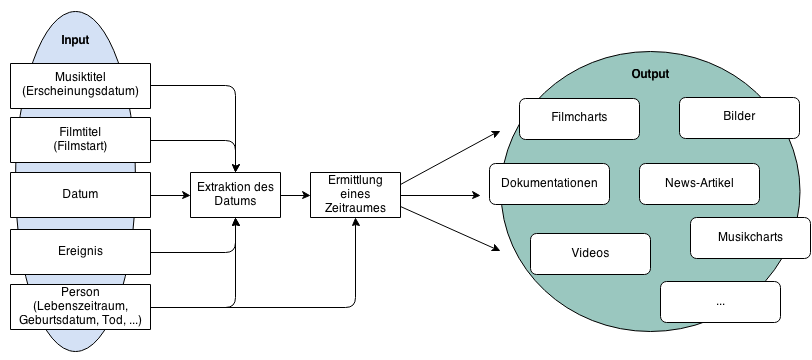
\includegraphics[width=1.0\textwidth]{Diagramm_Allgemein.png}
	\caption{Schematischer Ablauf der Suche}
	\label{fig:diagrammAllgemein}
\end{figure}

In Abbildung \ref{fig:diagrammVietnam} ist der schematische Ablauf mit der Beispiel-Eingabe \textbf{Vietnamkrieg} zu sehen. Aus der Eingabe leitet sich der Zeitraum 1955-1975 ab. Dieser Zeitraum wird daraufhin nach den popul�rsten Musik- und Film-Ver�ffentlichungen und wichtigen News-Artikeln durchsucht, um einen Querschnitt des Zeitraumes zu erstellen.
\begin{figure}[htb]
	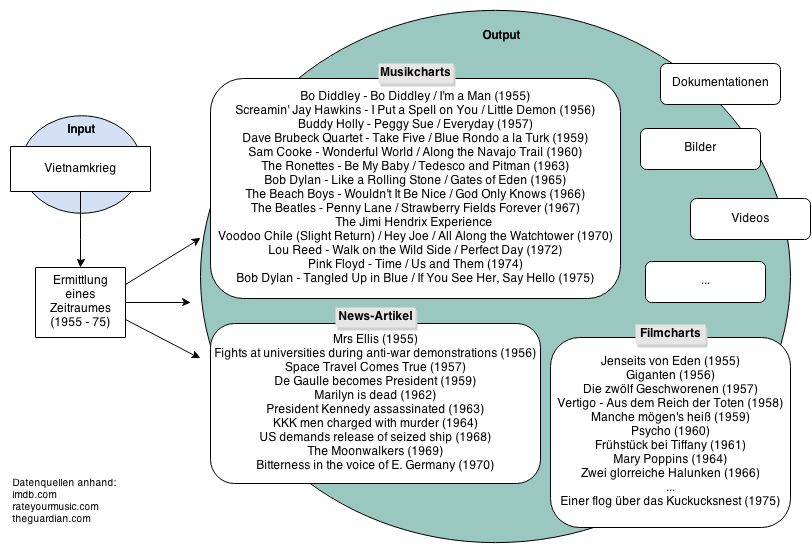
\includegraphics[width=1.0\textwidth]{Diagramm_VietnamKrieg.png}
	\caption{Schematischer Ablauf der Suche mit der Beispiel-Eingabe \glqq Vietnamkrieg\grqq}
	\label{fig:diagrammVietnam}
\end{figure}



%===== SECTION =====%
\section{Anforderungsanalyse}
Aus der vorangegangenen Analyse der vorhandenen Suchdienste geht hervor, dass eine umfassende Suche nach zeitspezifischen Inhalten bisher nicht besonders komfortabel ist, \bzw eine Suche oft nicht zuverl�ssig relevante Suchergebnisse liefert. Das liegt \va daran, dass die untersuchten Dienste, nicht darauf ausgelegt sind, zeitspezifisch zu suchen. Diese M�glichkeit soll die Web-Applikation, die im Rahmen dieser Arbeit entwickelt wird, bieten. �ber welche Funktionalit�t sie im Konkreten verf�gen soll, wird im Folgenden analysiert und anschlie�end in einer Feature-Liste dargelegt.

\subsection{Eingabeformen}
Ausgangspunkt f�r die Suche ist ihre Eingabeform. Der Nutzer soll hinsichtlich der Art seiner Eingabe m�glichst frei sein k�nnen. �ber die Text-Suche, wie sie in der vorangegangenen Analyse (siehe Kapitel \ref{cha:analyse}) durchgef�hrt wurde, gibt es noch weitere denkbare M�glichkeiten, welche im Folgenden erl�utert werden.

\paragraph{Datum}
Die Eingabe eines Datums ist die naheliegendste Suchform um zeitspezifisch nach Content, der sich auf den gew�hlten Zeitpunkt \bzw dessen umschlie�enden Zeitraum bezieht, zu suchen.

\paragraph{Ereignis, Zeitraum oder Epoche}
Prim�r sind Terme wie \zB \glqq 12.04.1922\grqq \ oder \glqq 1937\grqq \ denkbar, aus denen sich entsprechend der umschlie�ende Zeitraum ergibt. Dar�ber hinaus lassen sich viele Begriffe auch in Zeitr�ume oder Zeitpunkte aufschl�sseln, wie \zB die Begriffe \glqq Neunziger\grqq , \glqq Vietnamkrieg \grqq oder \glqq Deutscher Mauerfall\grqq . 

\paragraph{Musik oder Film}
Aus einer Musik- oder Film-Ver�ffentlichung kann ebenfalls ein Datum entnommen werden. Hier bietet sich beispielsweise das Ver�ffentlichungsdatum oder das Produktionsdatum an, w�hrend bei einer TV-Produktion die Erstausstrahlung und bei einem Kinofilm der Filmstart relevant ist. Dar�ber hinaus ist, soweit Informationen dar�ber vorhanden sind, die Popularit�t des Filmes von Interesse. Dies trifft \zB zu, wenn ein Musikst�ck oder ein Film erst deutlich nach der Ver�ffentlichung an Popularit�t gewinnt, \bspw aufgrund eines damit zusammenh�ngenden Ereignisses.

\paragraph{Bild oder Kunst}
Im Falle von Bildern oder Kunstwerken ist die Zuhilfenahme des Aufnahmedatums oder die Fertigstellung eines Kunstwerkes denkbar. Viele Kunstwerke \oae Items der weit zur�ckliegenden Vergangenheit lassen sich auf keinen genauen Zeitpunkt zur�ckdatieren, oftmals existiert in diesen F�llen ein m�glicher Zeitraum, in welchem ein Objekt fertiggestellt wurde oder eine Epoche, der es zugeordnet wird.

\paragraph{Personen}
Auch anhand eines Namens einer Person kann ein Zeitraum ermittelt werden. Dies kann, je nach Interesse, das Geburts- oder Todes-Datum, der gesamte Lebenszeitraum oder auch ein Zeitraum sein, in dem diese Person von gr��erer Popularit�t war (Amtsperiode, Aktivit�tszeitraum eines Musikers).

%----- SUBSECTION -----%
\subsection{Content-Typen}
Anhand eines Zeitpunktes oder -raumes lassen sich eine Vielzahl unterschiedlicher Inhaltstypen anzeigen. Da es das Ziel der Web-Applikation ist, ein m�glichst umfassendes Bild eines Zeitraumes anhand verschiedener Medien zu pr�sentieren, werden im Folgenden denkbare Inhaltstypen erl�utert.

\paragraph{Politische und geschichtliche Ereignisse}
Ein wichtiger Aspekt, der einen Zeitraum pr�gt, sind die darin auftretenden Ereignisse, die vom �ffentlichen Interesse sind. Zum einen sind politische Ereignisse wie \zB der \textit{Independence Day} der USA, der \textit{Mauerfall}, die Terroranschl�ge aber auch zeitpr�gende Begriffe wie die \textit{Goldenen Zwanziger}, die \textit{Industrialisierung} oder die \textit{Weltwirtschaftskrise} als Eingabe denkbar. Ebenso geh�ren Natur- und Medien-Ereignisse dazu. Hier kann als Beispiel die erste Landung eines Menschen auf dem Mond genannt werden. Ebenso interessant sind Informationen wie die Regierungsform oder die derzeitige Parlamentszusammensetzung.

\paragraph{Demografische Daten}
Demografische Daten geben ebenfalls Aufschluss �ber einen Zeitraum. Die Zusammensetzung der Bev�lkerung, ihre Dichte oder \zB das durchschnittliche Alter der Menschen sind Aspekte, die einen Zeitraum mit ausmachen. Genauso k�nnen Arbeitslosenquoten einen R�ckschluss auf die Zufriedenheit der B�rger zulassen. Dar�ber hinaus k�nnen Informationen �ber das vorherrschende Wetter oder Informationen �ber die Dauer des Tageslichts an einem bestimmten Tag von Interesse sein.

\paragraph{Musik}
Musik repr�sentiert einen gro�en Teil des kulturellen Aspekts eines Zeitraums. Musik aus einem bestimmten Zeitraum spiegelt nicht nur den Geschmack, sondern auch politische Neigungen wieder oder besch�ftigt sich mit aktuellen Themen, denkt man an den Song \textbf{Only Time}, der im Zuge der Terroranschl�ge vom 11. September an gro�er Popularit�t gewann. Dazu macht Musik einen Teil des vorherrschenden Stils aus.

\paragraph{Kunst}
Verschiedenste Arten von Kunst haben schon die fr�hesten Epochen der Menschheit gepr�gt. �hnlich wie die Musik spiegeln Kunstwerke ihrer Zeit nicht nur den Stil einer Epoche wieder. \glqq Die meisten Menschen sehen gern auf Bildern, was sie auch in der Wirklichkeit gerne ansehen w�rden. Das ist ganz nat�rlich.\grqq \ \citep[Vgl.][Seite 15]{gombrich2001} Damit verdeutlicht \citeauthor{gombrich2001} inwiefern die Kunst auch Bed�rfnisse einer Gesellschaft widerspiegeln kann.

\paragraph{Film}
Film ist zwar im Gegensatz zu den Bildenden K�nsten ein eher junges Medium, hat sich jedoch als wichtiges und popul�res Medium etabliert. Die Popularit�t eines Films kann R�ckschl�sse auf den Geschmack und Zeitgeist der Gesellschaft geben. Hinzu kann ein Film, der sich mit der Thematik aus der Vergangenheit besch�ftigt, im Nachhinein interessant oder gar wichtig sein, \bzw im Nachhinein an Wichtigkeit gewinnen. Dar�ber hinaus geben besonders neue Filmproduktionen ein Bild der Generationen wieder. So kann \zB der Film \textbf{Breakfast Club (1985)} einen Querschnitt der damaligen Jugend geben und der Film \textbf{Back to the Future (1985)} eine, wenn auch nicht ganz ernstgemeinte, Annahme der Zukunft widerspiegeln.

Hinzu kommen Video-Reportagen und -Berichte, die einen Zeitraum n�her betrachten und selbst ein Bild eines Zeitraumes oder Ereignisses darstellen. Sonstiges Video-Material, wie \zB Filmtrailer, lassen sich auch in diese Kategorie z�hlen.

\paragraph{Erfindungen und technische Errungenschaften}
Erfindungen, insbesondere technischen Ursprungs, haben bereits in der Vergangenheit gro�en Einfluss auf die Ver�nderung der Gesellschaft ausge�bt. Nicht nur die Erfindung des Buchdruckes, des Computers oder des Internets haben zu ihrer Zeit und dar�ber hinaus das Leben der Menschen ver�ndert. Ebenso interessant k�nnen zeitnahe Reaktionen und Annahmen zu solchen Erfindungen sein, geben sie \uU Aufschluss �ber die Haltung der Menschen gegen�ber der Fortschritte. So \zB die fr�he Annahme, dass Geschwindigkeiten von �ber 30 km/h dem menschlichen K�rper t�dlich schadeten, wie auch der Spiegel die Aussage des Bayrischen Medizinal-Kollegium zitiert: \glqq Die schnelle Bewegung dieser neuen Lokomotive mu� bei den Reisenden unfehlbar eine Gehirnkrankheit, eine besondere Art des gef�hrlichen Delirium furiosum erzeugen.\grqq \ \citep{spiegelDelirium}

\paragraph{Video-Spiele}
Im fortgeschrittenen Zeitalter ist auch eine Darstellung von Video-Spielen, die zu der Zeit erschienen sind, Bestandteil einer umfassenden Suchanfrage. Sie geben ebenfalls Aufschluss �ber die f�r den Suchzeitraum aktuellen technischen M�glichkeiten.

\paragraph{B�cher}
Zwar sind B�cher ein haupts�chlich in analoger Form vorliegendes Medium, jedoch gibt es fast ohne Ausnahme mindestens die wichtigsten Meta-Daten �ber B�cher auch im Internet. Der Wert und die Bedeutung eines Buches f�r einen Zeitraum ist insbesondere im digitalen Zeitalter nicht zu vernachl�ssigen. Weitere Ver�ffentlichungen in analoger Form sind ebenfalls f�r die Darstellung eines Zeitraumes denkbar, wie \zB Comics.

\paragraph{Trends}
�ber die genannten Punkte hinaus gibt es viele weitere Trends, die ihr Zeitalter oder ihre Epoche pr�gen. Dazu z�hlen popul�res Spielzeug, markantes Mobiliar oder etwa zeitpr�gende T�tigkeiten.

%===== SECTION =====%
\section{Features}
Die Kernfunktionalit�t der Web-Applikation ist die Suche nach Inhalten, die aus einem spezifischen Zeitraum stammen, \bzw sich mit diesem Zeitraum befassen. Dar�ber hinaus soll der Inhalt auf unterschiedliche Weise pr�sentiert werden und konsumiert werden k�nnen. Haupts�chlich soll eine visuell ansprechende Form der Inhalte pr�sentiert werden, gleichzeitig soll es dem Nutzer erm�glicht werden, direkt in der Web-Anwendung Audio-Inhalte zu h�ren, w�hrend er sich weitere Ergebnisse seiner Suche ansieht. Ebenso soll es m�glich sein, w�hrend des Durchst�berns der Suchergebnisse Video-Inhalte betrachten zu k�nnen.

%----- SUBSECTION -----%
\subsection{Standard Suche}
Eine Standard-Suche bezeichnet im Falle von \textbf{\arbeitstitel} eine Suche nach Inhalten aus einem vorgegebenen Zeitraum. Indem der Nutzer einen Zeitraum oder Zeitpunkt angibt, der entsprechend aufgel�st wird, wird in allen vorhandenen Quellen nach Inhalten gesucht und diese ungefiltert angezeigt.

%----- SUBSECTION -----%
\subsection{Thematisches Suchen}
W�hrend die Suche nach einem blo�en Datum stringent alle auffindbaren Informationen, die in den umschlie�enden Zeitraum fallen, anzeigt, muss es auch m�glich sein, gezielt thematisch zu suchen. Zum Beispiel soll es die M�glichkeit geben, ausschlie�lich Informationen eines Zeitraumes, die sich auf das Thema Musik beziehen, anzuzeigen. Dabei sind keinesfalls lediglich Musikdateien gemeint, sondern auch \bspw Text- oder Videoquellen, die sich mit dem Thema Musik besch�ftigen. Das Ergebnis w�re in diesem Falle ein Gesamtbild der derzeitigen Musikgeschichte. Die Ergebnisse einer solchen Suche sind stark abh�ngig davon, wie erfasst wird, ob ein Item dieses Thema behandelt und woran die Relevanz gemessen werden kann. Weitere m�gliche Beispiele einer thematischen Suche sind \zB Filmgeschichte oder Kunstgeschichte. Zur wissenschaftlichen Recherche bietet sich \zB an, das Thema Politik auszuw�hlen.
Als Beispiel kann zum einen Videomaterial einer politischen Rede, die in dem gew�nschten Zeitraum stattgefunden hat, zum anderen ein Zeitungsartikel, der sich mit einem bestimmten Musiktitel auseinandersetzt, dienen. Diese Funktionalit�t setzt die Unterscheidung zwischen Content, der zu gegebener Zeit produziert wurde, und Content, der sich auf diese Zeit bezieht und das vorgegebene Thema behandelt, voraus.

%----- SUBSECTION -----%
\subsection{St�bern in der Zukunft}
Faktisch sind Medien, die erst in der Zukunft produziert werden, noch nicht existent, jedoch gibt es bereits Medien-Items, die sich auf die Zukunft beziehen k�nnen. Ein Beispiel ist der Film \textbf{Back to the Future II}. Im zweiten Teil der Trilogie reist der Protagonist in das Jahr 2015. Somit ist der Film, auch wenn er ein imaginatives 2015 darstellt, trotzdem relevant f�r das Jahr 2015.


%----- SUBSECTION -----%
\subsection{Eingrenzen der Suche}
Um den Nutzen der Web-Applikation m�glichst vielseitig zu halten, kann bei der Suche die Art des Inhalts eingegrenzt werden. So kann die Wahl getroffen werden, welche Medientypen angezeigt werden sollen (Audio, Video, Text etc.). Auch ist eine Filterung der in Betracht gezogenen Dienste denkbar, sodass der Nutzer \bspw bestimmte APIs deaktivieren kann. Die Suche liefert im besten Fall ein gro�es Spektrum an Daten. Um ein genaueres Bild von einem Zeitraum zu bekommen, kann der User bereits beim Suchen spezifizieren, welche Inhalte ihm angezeigt werden sollen. 
Die Suche kann \ua nach Medientypen eingegrenzt werden. Hier empfiehlt sich eine Eingrenzung nach Medientypen und -arten. Steht bei der zeitspezifischen Suche \bspw eine wissenschaftliche Recherche im Vordergrund, empfiehlt es sich, die Suche auf Text- oder Tabellen-Items zu begrenzen. Will der Nutzer haupts�chlich den Unterhaltungsaspekt von \arbeitstitel \ nutzen, kann er die Suche auf Audio und Video begrenzen, wobei es sich bei den Medientypen \ggf anbietet, diese weiter eingrenzen zu k�nnen. M�chte sich der Nutzer beispielsweise nur einen Radiosender generieren lassen und w�nscht keinen Video-Content, kann der Nutzer das Ergebnis weiter einschr�nken. Eine Aufschl�sselung der Medientypen und ihrer Subtypen ist in Tabelle \ref{tab:mediaTypes} zu sehen.


\begin{table}[H]
	\begin{center}
		\begin{tabular}{|c||c c c c c|}
		  %Medientyp & bla & bla \\ \hline\hline
		  \hline
		  Medientyp & &  & Sub-Typen & & \\ \hline\hline
		  Text & News-Artikel & Bericht & Buch & Definition & Prosa/Lyrik \\ \hline
		  Audio & Musik & Podcast & Radio-Sendung & H�rspiel & \\ \hline
		  Video & Film & Reportage & TV-Sendung & Trailer & \\ \hline
		  Bild & Fotografie & Gem�lde & Zeichnung & & \\ \hline
		  Grafik & Tabelle & Diagramm & Visualisierung & & \\ \hline
		\end{tabular}
		\caption{Medientypen und ihre Sub-Typen}\label{tab:mediaTypes}
	\end{center}
\end{table}

Um �ber l�ngere Zeit auch eine zuverl�ssige wissenschaftliche Recherche zu erm�glichen, kann es von Nutzen sein, bei der Suche bestimmte Dienste zu ex- \bzw inkludieren. Dies kann \va dann von Interesse sein, wenn das Ergebnis m�glichst unabh�ngig von den bestimmten APIs sein soll. Die Beschr�nkung der Suche nach Quellen, APIs und anderen Suchdiensten wird \va dann interessant, wenn es f�r einen Medientyp verschiedene Quellen gibt. Insbesondere wenn die Quellen verschiedene Genres abdecken oder auf bestimmte Bereiche spezialisiert sind. Das ist \zB im Kunstbereich der Fall, wie aus der vorangegangenen Analyse hervorgeht, dessen Online-Angebot meist auf die jeweilige Galerie begrenzt ist. Ein weiteres Beispiel f�r den Bereich Musik sind Musikdienste, die sich auf spezielle Musikrichtungen spezialisiert haben. Au�erdem k�nnen die Ergebnisse von Interesse sein, wenn popul�re Quellen, APIs und sonstige Suchdienste nicht mit einbezogen werden um zu vergleichen, zu welchen Anteilen diese die Zusammensetzung des Suchergebnisses beeinflussen.

\subsection{Filtern des Ergebnisses}
Ein weiteres Feature ist die Filterung der Ergebnisse nach verschiedenen Kriterien. Daf�r m�ssen die gesammelten Informationen jedoch Grundvorraussetzungen erf�llen, um diese Kriterien �berhaupt bedienen zu k�nnen. Das Filtern nach Genre bietet sich \bspw bei Musik an, da diese Informationen gr��tenteils bereits in den untersuchten Datenbanken vorhanden sind. In diesem Fall kann \zB nach Musik-Genres wie Rock, Pop, Klassik oder Hip-Hop gefiltert werden. �hnlich verh�lt sich das Filtern bei Filmen. Insbesondere, wenn der Nutzer die Suche im Vorfeld auf den Medientyp Video und die Sub-Kategorie Film reduziert hat, bietet sich an, diese Auswahl nachtr�glich nach Action, Drama oder \bspw Thriller zu filtern. 

Dies ist f�r andere Medientypen entsprechend schwieriger umzusetzen, da es eigens betitelte Genres gibt und diese in den seltensten F�llen gepflegt sind und dar�ber hinaus maschinell auswertbar sind.

Der Grund, die Ergebnisse in zwei Schritten und in dieser Art zu filtern und zu verfeinern, liegt in der Art der Abfrage der Daten. Wird nach einem Zeitraum gesucht, k�nnen bestimmte Medientypen und \ggf bestimmte Quellen direkt ausgeschlossen werden. Daraus ergibt sich erst die M�glichkeit, inwiefern eine Filterung des Ergebnisses �berhaupt machbar ist. In diesem Fall ist die Funktionalit�t davon abh�ngig, in welcher Form die Daten vorliegen. Wurden bei der Suche bereits Items gefunden, die \bspw �ber Informationen wie Genre, Stil \oae verf�gen, kann diese M�glichkeit erst angeboten werden. Ansonsten w�re es f�r den Nutzer frustrierend und auch kompliziert ein Suchergebnis zu filtern, wenn dieser letztendlich gar keinen Einfluss auf die Zusammensetzung des Ergebnisses aus�ben kann, weil dies technisch nicht m�glich ist.

\paragraph{Ort}
Eine Suchanfrage kann spezieller gestellt werden, in dem sie mit einer Ortsangabe erweitert wird. Das kann zum Beispiel mit der zus�tzlichen Angabe eines Ortes geschehen. Hier w�rden \zB Musik-Charts des jeweiligen Landes durchsucht oder demografische Daten angezeigt.

\paragraph{Genre}
Insbesondere bei Audiodaten finden sich in den ID3-Tags Informationen �ber das Genre des Musikst�ckes. Konnten mehrere Genres ausgemacht werden, k�nnen die gefundenen Items nach Genre gefiltert werden.

\subsection{Zeitspezifizierung} %oder 
%----- SUBSECTION -----%
%\subsection{Zeitraum eingrenzen}

Mit der Grundeinstellung wird der Zeitpunkt als Zeitraum durchsucht. \Dahe dass vom Zeitpunkt ausgehend nach Medien in der nahen Vergangenheit, als auch in der nahen Zukunft gesucht wird. Au�erdem kann der Zeitraum, in dem gesucht wird, eingegrenzt werden. Zum einen kann vom Zeitpunkt ausgehend gesucht werden, sodass nur Items ab dem angegebenen Zeitpunkt angezeigt werden, oder andersherum nur Items angezeigt werden, die zu dem Zeitpunkt und davor existierten.

Im Fokus der Applikation steht der Zeitpunkt, der dargestellt werden soll. Dementsprechend soll es dem Nutzer m�glichst offen stehen, wie er seine Suche formuliert, solange der Suchbegriff sich in einen Zeitpunkt aufl�sen l�sst. Von diesem Zeitpunkt l�sst sich, je nach Dichte der Suchergebnisse ein Zeitraum ermitteln, \dahe dass vom Zeitpunkt ausgehend die relevantesten Treffer angezeigt werden. Je mehr Ergebnisse in der Suche angezeigt werden, desto gr��er spannt sich der Zeitraum, der dargestellt wird.

%----- SUBSECTION -----%
\subsection{Sortieren}
\paragraph{Relevanz}
Ohne Spezifierung einer Sortierung werden gefundene Items nach Relevanz sortiert. Das bedeutet, dass von jeder Datenquelle das erste Ergebnis als erstes im Suchergebnis auftaucht. Die Reihenfolge der Datenquellen ist zuf�llig. Bei einer Einbindung passender Algorithmen, die das Messen der Relevanz eines Items erm�glichen, ist auch eine zus�tzliche Sortierung innerhalb der Web-Applikation denkbar. Dies setzt voraus, dass die Ergebnis-Items �ber gen�gend Informationen verf�gen, die f�r das Messen der Relevanz n�tig sind.

\paragraph{Datum}
Die Ergebnis-Items k�nnen chronologisch oder umgekehrt-chronologisch sortiert werden. Diese M�glichkeit entf�llt, wenn die Such-Parameter dies ausschlie�en. Wenn \bspw nach Inhalten eines spezifischen Datums gesucht wird, ohne den umschlie�enden Zeitraum in Betracht zu ziehen, k�nnen die Items nicht sortiert werden.

\paragraph{Medientyp}
Inhalte k�nnen nach Medientypen sortiert werden, sodass \bspw zuerst Audio-, dann Text- und dann Video-Inhalte angezeigt werden. Dar�ber hinaus ist eine Sortierung nach Medien-Subtypen oder Datenquellen denkbar, die der Nutzer \bspw durch \textbf{Drag and Drop} in der Sortierungs-Maske anordnen kann.

\section{Use Cases}
Zur Aufschl�sselung des Funktionsumfangs, wird im Folgenden eine Auswahl von Anwendungsf�llen aufgelistet.

\paragraph{Suche nach Inhalten anhand eines Zeitpunktes} Suche nach Inhalten aus dem Jahre 1948.
\begin{enumerate}[1.]
	\item User gibt \glqq 1948\grqq \ in das Suchfeld ein
	\item System sucht nach Items, die zum Suchbegriff passen und sich in einen Zeitraum �bersetzen lassen
	\item User w�hlt den passenden Zeitraum durch die Auswahl des Items \glqq Datum - 1948\grqq \ aus
	\item System sucht nach Items unterschiedlichen Medientyps
	\item Frontend zeigt Musik-, Film-, Text-Items etc. aus dem Jahre 1948 an
\end{enumerate}

\paragraph{Suche nach Video-Inhalten anhand eines Ereignisses} Suche nach Video-Inhalten zur Zeit der Terroranschl�ge am 11. September 2001
\begin{enumerate}[1.]
	\item User gibt \glqq September 11 attacks\grqq \ in das Suchfeld ein
	\item User grenzt die Suche nach Medientyp \textbf{Video} ein
	\item System sucht nach Items, die zum Suchbegriff passen und sich in einen Zeitraum �bersetzen lassen
	\item User w�hlt den passenden Zeitraum durch die Auswahl des Items \glqq Ereignis - September 11 attacks - 11.9.2011\grqq \ aus
	\item System sucht nach Items unterschiedlicher Medienarten des Medientyps \textbf{Video}
	\item Frontend zeigt Reportagen-, Film-, TV-Sendungen-Items etc. des Datums 11. September 2001 an
\end{enumerate}

\paragraph{Suche nach Musik anhand eines Zeitpunktes eines Items} Suche nach Musik zur Zeit des Filmstarts von \textbf{Der Pate}.
\begin{enumerate}[1.]
	\item User gibt \glqq the godfather\grqq \ in das Suchfeld ein
	\item User grenzt die Suche nach Medientyp \textbf{Audio} und Medienart \textbf{Musik} ein
	\item System sucht nach Items, die zum Suchbegriff passen und sich in einen Zeitraum �bersetzen lassen
	\item User w�hlt den passenden Zeitraum durch die Auswahl des Items \glqq Film - The Godfather - 1972\grqq \ aus
	\item System sucht nach Items des Medientyps \textbf{Audio} mit dem Medien-Subtypen \textbf{Musik}
	\item Frontend zeigt Musik-Items etc. aus dem Jahre 1972 an
\end{enumerate}

\paragraph{Suche nach wissenschaftlichen Inhalten anhand eines Ereignisses} Suche nach Text-Inhalten w�hrend des \textbf{Kalten Krieges}.
\begin{enumerate}[1.]
	\item User gibt \glqq cold war\grqq \ in das Suchfeld ein
	\item User grenzt die Suche nach Medientyp \textbf{Text} und \textbf{Bild} ein und grenzt letzteres nach den Medien-Subtypen \textbf{Tabelle}, \textbf{Grafik} und \textbf{Diagramm} ein
	\item System sucht nach Items, die zum Suchbegriff passen und sich in einen Zeitraum �bersetzen lassen
	\item User w�hlt den passenden Zeitraum durch die Auswahl des Items \glqq Ereignis - Cold War - 1947-1991\grqq \ aus
	\item System sucht nach Items aller Medien-Subtypen des Medientyps \textbf{Text} und den Medien-Subtypen \textbf{Tabelle}, \textbf{Grafik} und \textbf{Diagramm}
	\item Frontend zeigt Zeitungsartikel, Berichte, Schaubilder \etc aus den Jahren 1947-1991 an 
\end{enumerate}

\paragraph{Thematische Suche anhand eines Zeitraumes und eines Themas} Suche nach musikgeschichtlichen Inhalten in den Siebzigern.
\begin{enumerate}[1.]
	\item User gibt \glqq 1970-1979\grqq \ in das Suchfeld ein
	\item User grenzt die Suche nach Thema \textbf{Musik} ein
	\item System sucht nach Items, die zum Suchbegriff passen und sich in einen Zeitraum �bersetzen lassen
	\item User w�hlt den passenden Zeitraum durch die Auswahl des Items \glqq Zeitraum - 1970-1979\grqq \ aus
	\item System sucht nach Items aller Medientypen, die sich mit dem Thema Musik befassen
	\item Frontend zeigt Items aller Medientypen, die sich auf Musik beziehen
\end{enumerate}


%==============================================================================%
%==============================================================================%
%==============================================================================%
%==============================================================================%
%==============================================================================%
%==============================================================================%


%===== SECTION =====%
\section{Grafische Darstellung}
Bei einer Darstellung so vieler verschiedener Arten von Daten, muss das Layout sowohl variabel, als auch konsistent sein. Die Breite der Inhalte kann sich sehr oft ver�ndern, wenn neue Quellen hinzugef�gt werden und eine bestimmte Darstellungsform erfordern. Gleichzeitig darf das Layout durch die Masse an unterschiedlichem Inhalt nicht an �bersichtlichkeit und Konformit�t einb��en.

Inhaltstypen m�ssen f�r den Benutzer klar erkennbar sein, sodass Audio-Daten schnell von Text-Daten \oae unterschieden werden k�nnen. Au�erdem soll der Nutzer komfortabel und unkompliziert durch die Ergebnisse navigieren k�nnen.


\subsection{Mockup}
Die Web-Applikation zeigt zu Beginn lediglich ein Suchfeld mit der M�glichkeit die Suche zu begrenzen.

\paragraph{Home - Disambiguation}
In Abbildung \ref{fig:homeDisambiguation} werden passende Suchvorschl�ge am Beispiel der Eingabe des Terms \glqq 2001\grqq \ angezeigt. Dies verdeutlicht ebenso den Umgang mit Disambiguierungen. So wird dem Nutzer angezeigt, welche Item-Typen gefunden wurden, Informationen �ber das Item selbst, wie \zB Titel oder Interpret, und letztendlich das Datum \bzw den Zeitraum, der durchsucht werden soll.

\begin{figure}[htb]
	\begin{center}
		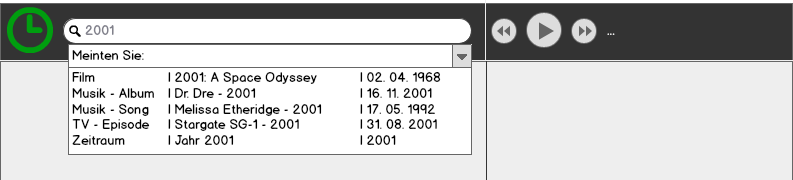
\includegraphics[width=1\textwidth]{mockup/u_1972_home_disambiguation_cropped.png}
		\caption{Home - Disambiguierung}
		\label{fig:homeDisambiguation}
	\end{center}
\end{figure}

\paragraph{Home - Suche eingrenzen}
In Abbildung \ref{fig:homeLimit} ist die Eingrenzung der Suche zu sehen, die der Nutzer vor der Suchanfrage vornehmen kann. Der Nutzer kann jede einzelne Medienart von der Suche aus- \bzw einschlie�en. Au�erdem kann der Nutzer durch das Klicken auf die Medientypen alle Subtypen automatisch mit ausw�hlen. In diesem Fall sind alle Subtypen ausgew�hlt und ausgegraut. Default sind alle Medien- und dessen Subtypen vorausgew�hlt.

\begin{figure}[htb]
	\begin{center}
		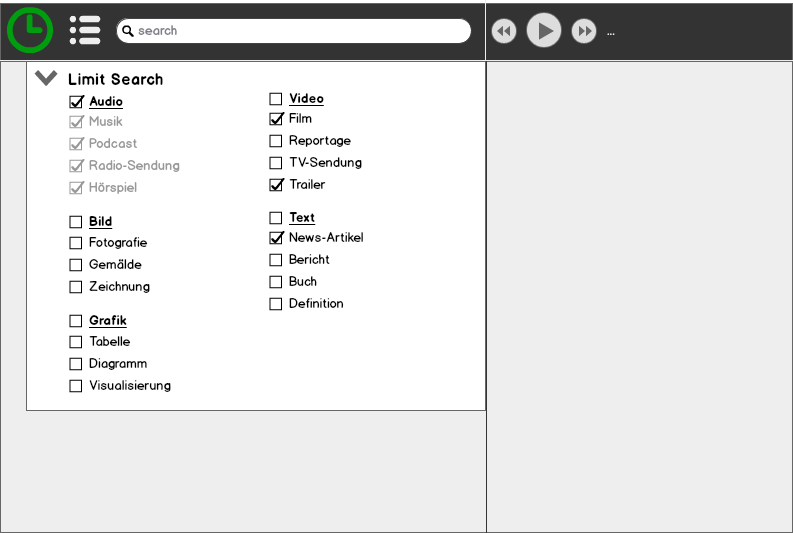
\includegraphics[width=1\textwidth]{mockup/u_1972_home_limit.png}
		\caption{Home - Suche eingrenzen}
		\label{fig:homeLimit}
	\end{center}
\end{figure}


\paragraph{Suchergebnis}
Die Abbildung \ref{fig:searchResult} zeigt das Suchergebnis bei einer Auswahl des Items \glqq David Bowie - Changes\grqq . Oben werden allgemeine Informationen �ber das Item angezeigt, \ua das Datum. Au�erdem werden weitere Informationen angezeigt, wie die h�chste Chart-Position der Single. 

Das Suchergebnis besteht aus Items der unterschiedlichen Medientypen. Die Items sind in einer gekachelten Ansicht angeordnet, wobei jedes Item anhand eines Bildes \zB Cover Art, Film Plakat \etc repr�sentiert wird, soweit vorhanden. Es sind sowohl Musikst�cke und Filme, als auch das Videospiel \textbf{Pong} aufgelistet. Text-Inhalte sind ebenfalls im Raster zu sehen, wobei ein Ausschnitt des Textes zu sehen ist. F�hrt der Nutzer mit der Maus �ber ein Item, werden ihm drei Icons angezeigt.

Im rechten Bereich ist die Playlist zu sehen, die alle abspielbaren Inhalte auflistet und anzeigt. Audio- und Video-Inhalte werden in der gleichen Reihenfolge, wie sie im Suchergebnis-Raster angezeigt werden, abgespielt, sobald der Nutzer auf Play klickt. Videos werden direkt im Playlist-Bereich eingebettet. Au�erdem k�nnen die Inhalte nach Belieben des Nutzers mittels Drag \& Drop in gew�nschter Reihenfolge abgespielt werden.

\begin{figure}[htb]
	\begin{center}
		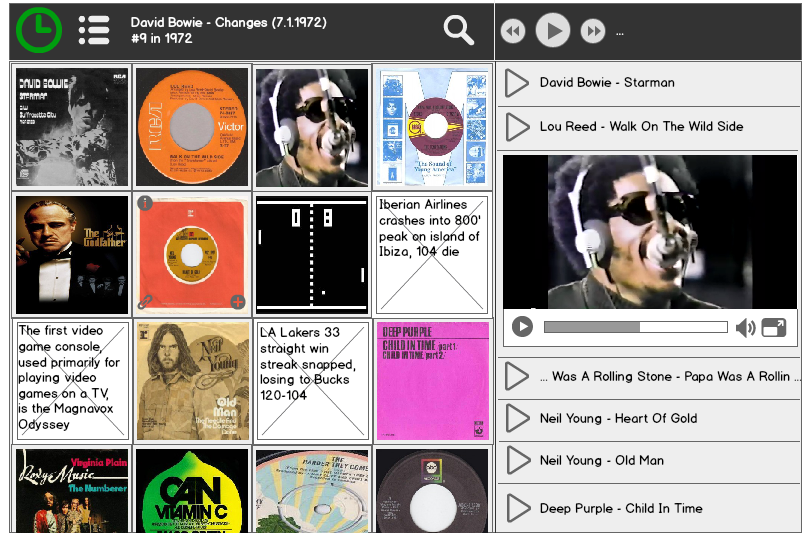
\includegraphics[width=1\textwidth]{mockup/u_1972_search_result.png}
		\caption{Suchergebnis}
		\label{fig:searchResult}
	\end{center}
\end{figure}

\paragraph{Suche - Details}
Mit Klick auf das Men�-Icon werden Details zum ausgew�hlten Items, an dessen Datum die Suche durchgef�hrt wurde, angezeigt. In Abbildung \ref{fig:searchDetails} sind das Album Cover, Titel, Interpret, Ver�ffentlichungsdatum, Genres und Chart-Position angezeigt.

\begin{figure}[htb]
	\begin{center}
		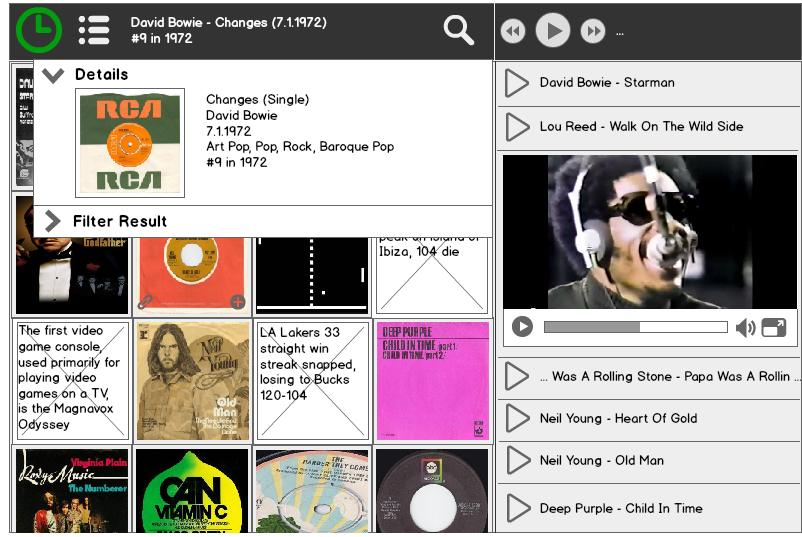
\includegraphics[width=1\textwidth]{mockup/u_1972_search_menu_details.png}
		\caption{Suche - Details}
		\label{fig:searchDetails}
	\end{center}
\end{figure}

\paragraph{Suchmen� - Filter}
Unter dem Men�-Eintrag \textbf{Filter Result} sieht man die M�glichkeiten zur nachtr�glichen Filterung des Suchergebnisses. In diesem Fall werden als m�gliche Genres \textbf{Art Pop}, \textbf{Pop}, \textbf{Rock} und \textbf{Baroque Pop} angeboten, da die Informationen durch den Online-Dienst erfasst werden k�nnen. Daneben kann der Zeitraum genauer spezifiziert werden.

\begin{figure}[htb]
	\begin{center}
		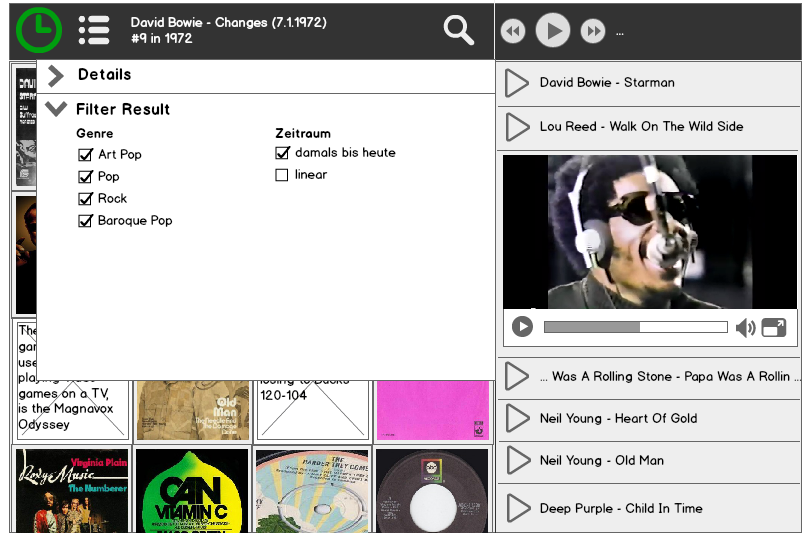
\includegraphics[width=1\textwidth]{mockup/u_1972_search_menu_filter.png}
		\caption{Suchmen� - Filter}
		\label{fig:searchFilter}
	\end{center}
\end{figure}

\paragraph{Suchergebnis - Cover-Info}
Bewegt der Nutzer die Maus �ber ein Item des Suchergebnisses, werden weitere Interaktionsm�glichkeiten mit dem Item eingeblendet. Dies beinhaltet die Anzeige von ausf�hrlicheren Informationen, das Hinzuf�gen eines Items zur Playlist -- sofern es sich um ein abspielbares Item handelt -- oder die Navigation zur Quelle des Items.
\begin{figure}[htb]
	\begin{center}
		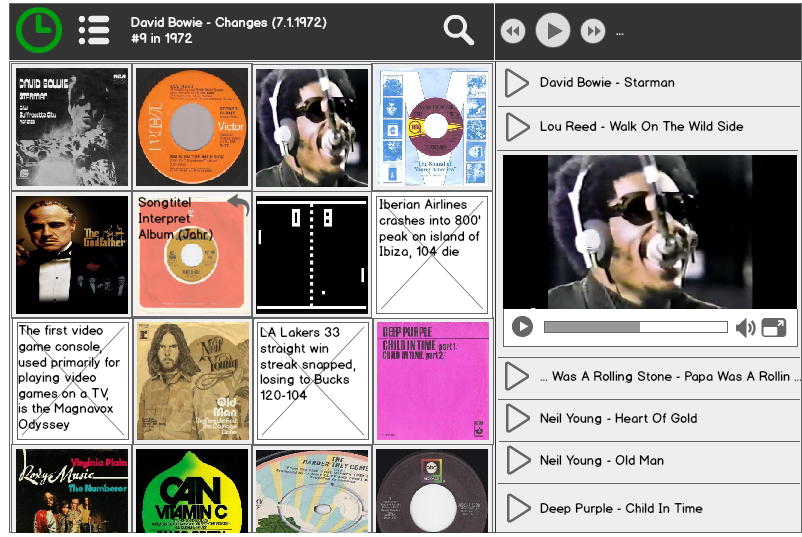
\includegraphics[width=1\textwidth]{mockup/u_1972_search_result_cover_info.png}
		\caption{Suchergebnis - Cover-Info}
		\label{fig:searchDetailsCoverInfo}
	\end{center}
\end{figure}


%----- SUBSECTION -----%
\subsection{Funktionalit�t}
Im Fokus der Applikation steht eine komfortable Suche, die dem Nutzer m�glichst einfach zug�nglich gemacht wird. Dies umfasst sowohl ein �bersichtliches Layout, als auch eine sinnvolle Auswahl an m�glichen Funktionalit�ten.
Eine f�r diese Web-Applikation besondere Aufgabe ist es, die drei Kernfunktionen m�glichst gleichzeitig gut erreichbar zu machen, ohne die Gesamterscheinung zu st�ren.

\paragraph{Suchen}
F�r eine m�glichst komfortable Suche werden schon bei der Eingabe im Suchfeld Suchvorschl�ge gemacht. Daf�r werden Such-Requests an die APIs der Suchdienste �bermittelt, um m�gliche Items vorzuschlagen.

\paragraph{Browsen}
Initial werden die aggregierten Ergebnis-Items nur anhand eines Bildes, Covers \oae repr�sentiert. Dar�ber hinaus kann sich der Nutzer weitere Details �ber das gefundene Item ansehen. Weiterhin kann die Quelle des Items eingesehen werden, indem der Source-Link des Inhaltes eingebunden und aufrufbar ist. Insbesondere Text-Inhalt, der �ber sehr gro�en Umfang verf�gt, kann so auf der Quell-Webseite gelesen werden. Au�erdem k�nnen bei Musiktiteln \bspw Chart-Informationen und andere Informationen angezeigt werden. 

Zudem kann der Nutzer ein ausgew�hltes Item aus den Suchergebnissen f�r eine weitere Suche ausw�hlen.

\paragraph{Konsumieren}
Unter den dargestellten Inhalten befinden sich auch abspielbare Inhalte. Diese soll der Nutzer sich m�glichst gleichzeitig anschauen und anh�ren k�nnen.

%----- SUBSECTION -----%
\subsection{Design und Layout}
Da die Web-Applikation sehr viele unterschiedliche Medienarten und -inhalte darstellen soll, ist ein �bersichtliches und klares Design erforderlich, um es dem Nutzer zu erm�glichen, sich auf die Inhalte konzentrieren zu k�nnen. Darum ist es wichtig, dass das Design m�glichst flexibel ist, unabh�ngig vom Inhalt. Folgende Aspekte sind beim Layout zu beachten:

\paragraph{Suche und Filter}
In der Eingrenzung der Inhalte wird unterschieden, welche Eingrenzungen vor dem Beginn der Suche stattfinden, und welche lediglich dem Filtern des Ergebnisses dienen. Das sind zum einen die Faktoren, die die Suche selbst ma�geblich beeinflussen. Zum anderen sind das Faktoren, die lediglich das vorhandene Ergebnis filtern.

\paragraph{Musik- und Video-Player}
W�hrend alle Suchergebnisse in einer Art Raster einheitlich angezeigt werden, gibt es f�r Audio- und Video-Inhalte zus�tzlich einen separaten Bereich, in dem diese nach Reihenfolge im Suchergebnis sortiert als Playlist bereit stehen. Das bedeutet, dass der Nutzer, w�hrend er im linken Bereich durch Inhalte verschiedener Medientypen scrollt, im rechten Bereich die automatisch erstellte Playliste angezeigt wird und dementsprechend die Inhalte betrachtet, \bzw angeh�rt werden k�nnen. Au�erdem k�nnen einzelne Items der Playliste durch Drag \& Drop neu angeordnet oder Items von der Playliste entfernt werden. Mit Klick auf das Queue-Symbol eines Items, wird das gew�hlte Item an n�chster Stelle in der Liste platziert und als n�chstes abgespielt. Wird auf das Play-Symbol eines Items geklickt, wird dieses sofort abgespielt.


%===== SECTION =====%
\section{Eingrenzung}
Die Masse an unterschiedlichen Medien-Typen, -Quellen und -Arten, die in \arbeitstitel \ angezeigt werden kann, l�sst sich kaum erfassen. Je nach Belieben und sich neu er�ffnenden M�glichkeiten kann sich sowohl das m�gliche Angebot, als auch die Nachfrage nach bestimmten zeitspezifischen Content �ndern. Ein Gro�teil der denkbaren Daten sind zwar im Internet verf�gbar, jedoch fehlt es meist an komfortablen M�glichkeiten, diese insbesondere zeitspezifisch zu aggregieren.

Im Rahmen dieser Masterarbeit wird daher ein Working Prototype als Proof of Concept implementiert werden. In dieser Hinsicht wird die Funktionalit�t von \arbeitstitel \ auf die Medientypen Musik und Film reduziert werden. Zum Thema Musik gibt es eine Vielzahl an zuverl�ssigen und offenen Quellen, die f�r unkommerzielle Zwecke zur freien Verwendung zur Verf�gung stehen, au�erdem ist die Art der vorliegenden Daten, insbesondere aufgrund des ID3-Standards, der Entwicklung zutr�glich. 			% 15-30 Seiten
% Konzeption
%	"Fernkonzept"
%	Mockup
%	Eingrenzung
%!TEX root = ../Masterarbeit.tex
\chapter{Implementierung}
\label{cha:implementierung}

\section{Quellen}
%Erforderliche und ben�tigte Quellen und APIs
Im folgenden Abschnitt werden in Frage kommende Quellen und APIs und deren Vor- und Nachteile in Hinsicht auf Verwendung innerhalb der Web-Applikation \arbeitstitel \ vorgestellt. Untersucht werden nicht nur APIs, sondern auch andere m�gliche Formen, um an die ben�tigten Daten f�r eine Suche innerhalb \arbeitstitel \ zu gelangen.

\subsection{Musik}
\subsubsection{MusicBrainz}
MusicBrainz ist eine offene Musik-Enzyklop�die, die f�r Mensch und Maschine lesbare Informationen �ber Musik �ffentlich zug�nglich macht \citep[Vgl.][]{musicbrainz}. Sie enth�lt umfangreiche Daten �ber K�nstler und deren ver�ffentlichte Musik, insbesondere auch Informationen �ber einzelne Erscheinungen. Dar�ber hinaus verf�gt MusicBrainz auf den K�nstler-Profilen �ber s�mtliche Verweise zu weiteren Referenzen im Internet wie Wikipedia-Artikel, Youtube-Channel, Facebook-Seite, Wikidata-Eintrag \uvm 

MusicBrainz verf�gt �ber eine offene API, die f�r unkommerzielle Zwecke kostenlos genutzt werden darf. Sie bietet die Entit�ten \texttt{lookup}, \texttt{browse} und \texttt{search} an. Es bieten sich insbesondere die Subqueries von \texttt{artist}, \texttt{recording}, \texttt{release} und \texttt{release-group} an. Es gilt zu beachten, dass bei einem \texttt{search}-Request der gew�nschten Ergebnistyp definiert werden muss. So m�ssen f�r eine Suche, wo nicht klar ist, ob der Interpret, Titelsong oder Album eingegeben wurde, zwei Queries durchgef�hrt werden.

Seperat bietet MusicBrainz den Service Cover Art Archive an, �ber den man anhand von MusicBrainz-IDs an Album Art der Releases abfragen kann.


\subsubsection{RateYourMusic}
RateYourMusic ist wie MusicBrainz ebenso eine durch Nutzer gepflegte offene Datenbank, die �ber Musikdaten hinaus auch Daten �ber Film bietet \citep[Vgl.][]{rym}. Ein f�r \textbf{\arbeitstitel} interessantes Feature ist die M�glichkeit sich Charts anzeigen zu lassen, und diese nach diversen Kriterien wie Genre oder Zeit zu filtern. Leider verf�gt RateYourMusic �ber keine API und verbietet auch ausdr�cklich das Scrapen der Daten auf ihrer Website.

\subsubsection{OneMusicAPI}\label{subsubsec:OneMusicAPI}
OneMusicAPI ist eine API, die auf der Software von Bliss basiert \citep[Vgl.][]{oneMusicAPI}. W�hrend Bliss das automatische Nachladen von Cover Art erm�glichen soll \citep[Vgl.][]{bliss}, sind mit OneMusicAPI Requests mit Interpret und Songname nach Release m�glich. Dies stellt auch einen Nachteil dieser API dar, da Song-Informationen nicht so umfangreich sind, wie die anderen vorhandenen Datenbanken und au�erdem nur nach Informationen gefragt werden kann, wenn Interpret und Songtitel bekannt sind. Au�erdem ist die API nach 1000 Lookups kostenpflichtig.

\subsubsection{Music Story Pro}
Music Story Pro \citep[Vgl.][]{musicStoryPro} ist wie OneMusicAPI (\ref{subsubsec:OneMusicAPI}) nur begrenzt kostenlos verf�gbar. Zum einen ist die Anzahl der Requests auf 50000 pro Monat begrenzt, weiterhin ist die volle Funktionalit�t nur f�r zahlende Kunden verf�gbar. Dies beinhaltet \zB Review-Informationen und Bilder. Ein Vorteil bei Music Story Pro ist, dass eine Schnittstelle f�r weitere APIs bietet. Dazu geh�ren \ua \ Spotify, Deezer, iTunes und Amazon. Au�erdem implementiert es die Suche von MusicBrainz, indem es sowohl \gls{Release} als auch \gls{ReleaseGroup} im MusicBrainz-Format liefert.

\subsection{Discogs}
Discogs hat es sich zur Aufgabe gemacht die gr��te und umfangreichste Musikdatenbank, inkl. Market Place bereitzustellen \citep[Vgl.][]{discogs}. Au�erdem stellt Discogs eine API bereit, die nicht nur das Durchsuchen des Datenbestandes erm�glichen, sondern auch den MarketPlace durchsuchen lassen. Im Gegensatz zu den anderen Musikquellen, ist der soziale Charakter bei Discogs au�erdem ausgepr�gter.

\subsection{Film}
\subsubsection{IMDb}
IMDb ist die verbreiteste Filmdatenbank im Internet. IMDb enth�lt �ber Filmdaten hinaus auch Informationen �ber alle Mitwirkenden, Bewertungen, Plots \uvm Eine offizielle API bietet IMDb derzeit nicht, jedoch werden auf der Seite die Daten in Textform zum Download bereitgestellt, welche f�r unkommerzielle Zwecke genutzt werden d�rfen.

\subsubsection{themoviedb.org}
The Movie Database ist eine offene Film- und TV-Datenbank, die urspr�nglich auf Daten der Open Media Database \citep{omdb} entstanden ist und dar�berhinaus auf nutzergenerierten Inhalten basiert \citep[Vgl.][]{tmbd}. Au�erdem bietet TMDb eine unkommerziell verwendbare API f�r Entwickler, die sehr gut mit apiary dokumentiert ist.

\subsubsection{RottenTomatoes}
Rotten Tomatoes \citep{rottenTomatoes} ist eine Sammlung von Filmkritiken und bietet in diesem Zuge auch detaillierte Informationen �ber Film- und TV-Produktionen \citep[Vgl.][]{rottenWiki}.


\subsection{Gemischt}
\subsubsection{Wolfram|Alpha}
Wolfram|Alpha \citep{wolframAbout} bietet eine begrenzt kostenlose API. So ist eine kostenlose Verwendung f�r unkommerzielle Testzwecke auf 2000 API-Calls pro Monat begrenzt \citep[Vgl. How much I may use the Wolfram|Alpha API?][]{wolframAPIAbout}. Insbesondere das Thema \glqq People \& History\glqq \ \citep{wolframTopicHistory} ist f�r \arbeitstitel \ von Interesse, da das Aufl�sen von Historischen Ereignissen sowie Personen zu einem Zeitraum damit erm�glicht werden kann. Speziell Geburtsdaten, Todesdatum und Amtsperioden lassen sich �ber das Auslesen der sogenannten \texttt{Pods} \citep[Vgl. Basics of Wolfram|Alpha Output][]{wolframAPIDocumentation} erfassen.

\subsubsection{Wikipedia}
Wikipedia ist ein Online-Nachschlagewerk und bietet laut eigener Angabe \glqq rund 30 Millionen Artikel [...] in �ber 280 Sprachen\grqq \ \citep[Vgl.][]{wikiWiki}. Im Gegensatz zu Google und Wolfram|Alpha verfolgt die Wikipedia die Idee einer kollaborativen Enzyklop�die, was sich auch in der Lizensierung niederschl�gt, da sie unter der Creative-Commons-Attribution-ShareAlike-Lizenz weiter verwendet werden darf. Ein Nachteil ist wiederum, dass es einen gro�en Aufwand bedeutet, die Daten �ber Techniken wie scrapen oder parsen auszulesen.

\subsubsection{Marvel API}
Eine weitere API, die sich \va aufgrund des Inhaltes f�r die Verwendung in \arbeitstitel \ anbieten w�rde, ist die Marvel API \citep{marvel}. �ber diese lassen sich insbesondere inhaltliche Informationen �ber Marvel-Comics ermitteln. Leider gibt dar�berhinaus keine Informationen �ber Erscheinungsdaten \oae verwertbare Daten, die sich zeitlich einordnen lassen. Das schlie�t derzeit auch eine Verwendung dieser API �ber den Umweg aus, popul�re Comics anderweitig zu suchen und spezifische Daten von dieser API nachzuladen.

\section{Dienste}
Im Folgenden werden die Dienste vorgestellt, die verwendet werden k�nnen, um Audio- und Video-Content in der Playlist von \arbeitstitel, wenn auch lediglich repr�sentativ oder als Verlinkung darzustellen.
\subsection{Video}
\paragraph{Trailer}
Filme in \arbeitstitel \ einzubinden oder gar anzuzeigen, ist allein urheberrechtlich nicht erlaubt. Repr�sentativ k�nnen jedoch Trailer, soweit diese online frei vorhanden sind, verwendet werden. Trailer werden oft von den Film-Produktionsfirmen selbst online zur Verf�gung gestellt, um sie online leichter verbreiten zu k�nnen und den Film einer breiteren Masse bekannt zu machen. F�r diesen Zweck bietet TrailerAddict \citep{trailerAddict} eine API, die das embedden von Trailern vereinfacht. F�r die Darstellung von Trailern �ber TrailerAddict ist jedoch Flash 9 erforderlich \citep[Vgl.][]{trailerAddictAbout}, was \uU gro�e Restriktionen nach sich zieht, sollte der User kein Flash installiert haben.

\paragraph{YouTube}
Zum Einbetten von Musikvideos, Filmen und Film-Trailern bietet sich im Playlist-Bereich das Einbinden von YouTube-Videos \citep{youtube} an. Die YouTube-API kann �ber die Verwendung der Upload-Dienste hinaus auch f�r das Suchen von Videos oder Playlists verwendet werden \citep[Vgl.][]{youtubeAPI}.

Ein Problem, welches gegen die Verwendung von YouTube-Inhalten spricht, sind die vermehrten blockierten Inhalten aufgrund von Urheberrechtsanspr�chen, was insbesondere in Deutschland eine Vielzahl nicht abspielbarer Videos bedeutet.

% You can use the API to fetch search results and to retrieve, insert, update, and delete resources like videos or playlists.


\paragraph{Vimeo}
Vimeo \citep{vimeo} ist ebenso wie YouTube ein Video-Dienst der das Uploaden von Videos mit der sozialen Komponente verbindet. Vimeo bietet derzeit drei verschiedene APIs an. Die derzeit offizielle API gibt es in zwei Versionen, die \textbf{Simple API} \citep[][Vimeo Simple API]{vimeoAPIsSimple} und die \textbf{Advanced API}  \citep[][Vimeo Advanced API]{vimeoAPIsAdvanced}. Momentan arbeitet Vimeo an einer neuen API, die bereits verwendet werden kann, aber sich noch im Beta-Stadium befindet \citep[][Vimeo API (Beta)]{vimeoAPI}. 

Besonderheit ist, dass Vimeo dar�berhinaus noch eine als \textbf{JavaScript API} \citep[][Vimeo JavaScript API]{vimeoJSAPI} deklarierte API bereitstellt, die insbesondere die Steuerung des Vimeo-Players erm�glicht. Diese Funktionalit�t kann f�r die Realisierung des Players genutzt werden. 

Der gro�e Nachteil von Vimeo \bzgl der Nutzung f�r \arbeitstitel \ ist allerdings, dass Vimeos Kernaufgabe ist, eine Plattform f�r Videos, die \va k�nstlerischer Natur sind, zu bieten. D.h., es gibt zwar Musikvideos und Film-Trailer, jedoch nicht in der ausgepr�gten Form von YouTube.


%\paragraph{Sonstige}


\subsection{Audio}
\paragraph{Spotify}
�ber den kommerziellen Streaming-Dienst Spotify l�sst sich �ber ein musikalisches Repertoire bekannter Plattenlabels auf einer Vielzahl von Desktop- und Mobil-Ger�ten verf�gen. Spotify verf�gt �ber eine API, �ber die sich die verf�gbaren Musiktitel durchsuchen und einbetten lassen k�nnen. Aufgrund des Freemium-Konzepts ergibt sich der Nachteil, dass ein Nutzer von \arbeitstitel \ �ber einen Spotify-Account verf�gen muss, m�chte er unbegrenzt �ber die Web-Applikation Musik h�ren.

\todo{bissl details zur API, wie funzt das von ner suche eines titels zu nem embed-song im iframe}


\section{Techniken}
Zum Erfassen unterschiedlichster Daten im Internet gibt es verschiedene M�glichkeiten, wobei diese stark vom Angebot des Web abh�ngig sind. Im Folgenden werden diese Techniken vorgestellt und analysiert in unter welchen Umst�nden sie zu bevorzugen sind.

\subsection{Web-Services}
Web-Services folgen nicht zwangsweise den gleichen Gestaltungsgrunds�tzen und basieren nicht auf den gleichen Kern-Formaten oder Protokollen, obwohl sie sich im Web bereits durchgesetzt und sich als erfolgreich erwiesen haben \citep[Vgl. Seite 67][]{Fensel2011}. Im Folgenden werden die Standards kurz hinsichtlich ihrem Zweck f�r \arbeitstitel \ vorgestellt, sollten diese bei der Implementierung eine Rolle spielen.

\paragraph{SOAP}

\paragraph{RESTful-API}
Ein Gro�teil der im Internet verf�gbaren APIs basiert auf dem RESTful-Standard f�r Web-Anwendungen.


\subsection{Wrapper}


\subsection{Web-Scraping}
Das Web-Scraping ist eine Technik, mit der Informationen einer Webseite gesammelt werden k�nnen. Die f�r \arbeitstitel \ in Frage kommende Art des Web-Scraping ist das Herunterladen eines externen Quelltextes via HTTP, der Informationen, insbesondere �ber Film- oder Musikcharts verf�gt.

\subsection{Sweble}
\subsection{Download/Dumps}
Auf Wikipedia existieren brauchbare Seiten, die jeweils die Musik- und Film-Charts f�r jedes verf�gbare Jahr enthalten. Diese Vorgehensweise ist jedoch manuell aufw�ndig, da Informationen erst manuell herausgesucht werden m�ssen und nach den Vorgaben von Wikipedia �ber die Webseite bereitgestellte Funktion in Text-Dateien exportiert werden m�ssen. Diese Textdateien m�ssen geparst werden, wobei das Parsen der Daten in der von Wikipedia genutzten Skriptsprache Lua relativ unkomfortabel ist. Um das Editieren von Wikipedia-Artikeln einer breiten Masse m�glich zu machen, ist Lua mit seiner einfachen Syntax von gro�em Vorteil. Daf�r ist der Text nahezu zusammenhangslos und semantisch nicht automatisch auswertbar.

\medskip
%!TEX root = ../../Masterarbeit.tex
% \begin{lstlisting}[caption=Auszug eines Wikipedia-Artikel Downloads, label=lst:wikiUrl]
% http://en.wikipedia.org/w/index.php?title=Special:Export
% \end{lstlisting}

\begin{lstlisting}[caption=Auszug eines Wikipedia-Artikel Downloads, label=lst:wikiExcerpt]
{| class=&quot;wikitable&quot;
!Position !! Song !! Artist
|-
|1 || &quot;[[Blue Tango]]&quot; || [[Leroy Anderson]]
|-
|2 || &quot;[[Wheel of Fortune (1952 song)|Wheel of Fortune]]&quot; || [[Kay Starr]]
|-
|3 || &quot;[[Cry (Churchill Kohlman song)|Cry]]&quot; || [[Johnnie Ray]] &amp; [[The Four Lads]]
|-
|4 || &quot;[[You Belong to Me (1952 song)|You Belong to Me]]&quot; || [[Jo Stafford]]
|-
|5 || &quot;[[Auf Wiedersehn Sweetheart]]&quot; || [[Vera Lynn]]
\end{lstlisting}

http://en.wikipedia.org/w/index.php?title=Special:Export


nicht dynamisch, manuelle Downloads n�tig, parsen von Textdateien

\subsection{Mergen von Daten / Multiple Requests f�r einen Datensatz}
Da die Verwendung von bereitgestellten APIs klar zu bevorzugen ist, da dies bedeutet sicher an konsistente und m�glichst umfangreiche Daten zu gelangen, diese jedoch nicht auf die Anspr�che von \arbeitstitel \ zugeschnitten sind, wird es an vielen Stellen n�tig sein, auch f�r einzige Datens�tze auf verschiedene Services zur�ckzugreifen.

\subsection{Begrenzung von Requests pro Sekunde in den unterschiedlichen APIs}
%\subsection{Begrenzung von Requests in Express}



\section{Architektur der Web-Applikation}
Die Web-Applikation wird serverseitig mittels Javascript umgesetzt. Die Software-Plattform Node.js \citep{nodejs} bietet ein einfaches Konzept zur Erstellung und Inbetriebnahme von skalierbaren Netzwerk-Applikationen. Im Bezug auf \arbeitstitel \ ist das event-driven Konzept von gro�em Vorteil, da die Kommunikation mit mehreren APIs um einiges beschleunigt werden kann, indem die API-Requests von der Asynchronit�t Gebrauch machen.

\subsection{Express.js}
Das Web-Application-Framework \textbf{Express.js} \citep{expressjs} wird verwendet, da es eine Palette von Funktionalit�t zur einfachen Implementierung von Web-Applikationen mit \textbf{node.js} bietet und trotzdem flexibel und leichtgewichtig ist. Es ist als Schicht zwischen Funktionalit�t und Frontend zu verstehen und agiert als API \citep[Vgl.][]{expressjs}. Das ist speziell f�r \arbeitstitel \ vom Vorteil, da die API somit auch f�r weitere Anwendungen verwendet werden kann.

\subsection{MongoDB und NoSQL}
MongoDB \citep{mongodb} ist eine dokumentenorientierte Datenbank. Im Gegensatz zu relationalen Datenbanken l�sst sich mit der NoSQL-Strategie eine flexible Datenstruktur erstellen. Das macht im Falle von \arbeitstitel \ besonders Sinn, da sich die Art und der Umfang der Daten, die verarbeitet werden, sehr schnell �ndern k�nnen. Au�erdem vereinfacht dies auch die Erweiterbarkeit der Web-Applikation.

\subsection{Frontend mit Jade und Stylus}
Im Frontend werden die Werkzeuge Jade und Stylus verwendet. Jade \citep{jade} ist eine Node Template Engine und vereinfacht das Schreiben von HTML-Code, indem es eine eigene Syntax implementiert. �ber die vereinfachte Schreibweise hinaus implementiert sie auch Iterationen, Bedingungen und Filter. Au�erdem k�nnen sogenannte Mixins implementiert und somit dessen Funktionalit�t wiederverwendet werden.

Stylus \citep{stylus} ist eine f�r Node entwickelte Sprache, deren Kompilat CSS ist. Die Syntax ist im Gegensatz zu CSS stark vereinfacht. Weiterhin bietet sie Funktionen wie die Deklaration von Variablen, Funktionen und Mixins.

\subsection{Code-Generierung mit Yeoman}
Das Ger�st der Web-Applikation wurde mittels \textbf{Yeoman} \citep{yeoman}, einem Scaffolding-Tool f�r Webapps, generiert. Der Workflow von Yeoman basiert auf den drei Tools \textbf{Yo}, \textbf{Grunt} \citep{grunt} und \textbf{Bower} \citep{bower}. Bower ist ein Package Manager f�r das Frontend, Grunt ein Task Runner, mit Hilfe dessen Automatisierungsprozesse und Build-Skripte ausgef�hrt werden k�nnen. Yo kann mittles verschiedener Generatoren und Konfigurationen den Boilerplate-Code einer Web-Applikation und ein passendes Grunt Skript generieren.

Im Falle von \arbeitstitel \ wurde der Yeoman-Generator \textbf{generator-express} \citep{yeoExpress} verwendet. Das generierte Projekt bereits aus einer MVC-Struktur und hat bereits MongoDB als Default-Datenbank vorkonfiguriert. 
\begin{itemize}
	\item NodeJS
	\item Yeoman
	\item Grunt
	\item Bower
	\item Stylus
	\item mongoose
\end{itemize}

\section{Umsetzung und verwendete Tools im Frontend}
Im Folgenden werden verwendete Libraries und deren Nutzen erl�utert.

\subsection{Select2}
\textbf{Select2} \citep{select2} ist eine konfigurierbare Implementierung einer Selectbox. Sie bietet neben dem einfachen Suchen und einer Autosuggest-Funktion bereits Features wie dem automatischen Nachladen von Remote Datasets und unterst�tzt infinites Scrollen \citep[Vgl.][]{select2}. Da Select2 auf jQuery basiert sind keine weiteren Includes erforderlich. Au�erdem ist es ebenfalls �ber \textbf{Bower} erh�ltlich.

\subsection{Font Awesome}
Die Library \textbf{Font Awesome} \citep{fontAwesome} bietet ein Set von derzeit 369 Icons zur Verwendung an. Sie l�sst sich mittels Bower installieren und kann nach dem Einbinden der CSS-Files durch die Verwendung der vorgegebenen CSS-Klassen verwendet werden. Dies bietet den Vorteil, dass die verwendeten Icons sowohl stilkonform, als auch von der anzeigbaren Gr��e ver�nderbar sind.

\subsection{Darstellung von Filmplakaten in unterschiedlichen Formaten}
Um das User Interface trotz verschiedener Medientypen und deren Repr�sentierung m�glichst aufger�umt und �bersichtlich zu halten, wurde die Darstellung der Medien-Items in Rasterform umgesetzt. Somit ist f�r jedes Item eine quadratische Anzeige vorgegeben. Dies funktioniert gr��tenteils f�r Album-Cover, da diese fast ausnahmslos ebenfalls im quadratischen Format vorliegen, ohne Darstellungsprobleme. Hier k�nnen allerdings unsch�ne Darstellungsfehler auftreten, da die Album-Cover in unterschiedlichen Gr��en verf�gbar sind. Diese lassen sich mit Angabe einer festen H�he und Breite durch CSS verhindern. 

Eine besondere Behandlung wird f�r die Darstellung von Filmplakaten ben�tigt. Diese liegen zwar gr��tenteils im Hochformat vor, jedoch gibt es auch hier Ausnahmen. Das Problem kann einerseits damit gel�st werden, indem ein Teil des Plakats in originaler Aufl�sung dargestellt wird. Jedoch sind die dargestellten Bildausschnitte der Filmplakate dadurch nicht zuverl�ssig aussagekr�ftig. In der Web-Applikation wird das Plakat nun unabh�ngig von der Gr��e, der Aufl�sung und des Formats immer auf eine Breite und eine H�he von jeweils 200px gestreckt, \bzw gestaucht.

\section{Umsetzung und verwendete Tools im Server}
\subsection{async}
Das \textbf{async}-Modul \citep{async} erlaubt eine bessere Kontrolle �ber asynchron ausgef�hrte Funktionalit�t. Da \arbeitstitel \ an vielen Stellen mit mehreren APIs kommunizieren muss, ist die Asynchronit�t zwar generell ein Vorteil, jedoch werden auch Anfragen ben�tigt, die von mehreren asynchronen Requests abh�ngig sind. \Dahe , dass einige Requests von teilweise mehreren Requests, die vorher durchgef�hrt werden m�ssen, abh�ngig sind. Mit async lassen sich Callbacks in vordefinierter Reihenfolge durchf�hren. Auch eine Serie von ein und dem selben Callbacks auf Werten aus einer Liste, ist m�glich, genauso lassen sich mehrere Requests gleichzeitig abarbeiten bis dann der finale Callback ausgef�hrt werden kann, wenn alle Vorbedingungen erf�llt worden sind.


\medskip
\begin{lstlisting}[caption=Async Beispiel]
async.parallel({
		music_result: function(callback){
			getMusicSuggestionsBySearchterm(searchterm, callback);
		},
		movie_result: function(callback){
			getMovieSuggestionsBySearchterm(searchterm, callback);
		}
	},
	function(err, results) {
		if(err){
			callback(err, searchterm);
		} else {
			var resultset = results.music_result.concat(results.movie_result);
			callback(null, resultset);
		}
	});
\end{lstlisting}

\subsection{node-rest-client}


\subsection{cheerio}
\textbf{Cheerio} \citep{cheerio}

\subsection{nodebrainz und coverart}

\subsection{node-imdb-api}


\begin{figure}[htb]
	\begin{center}
		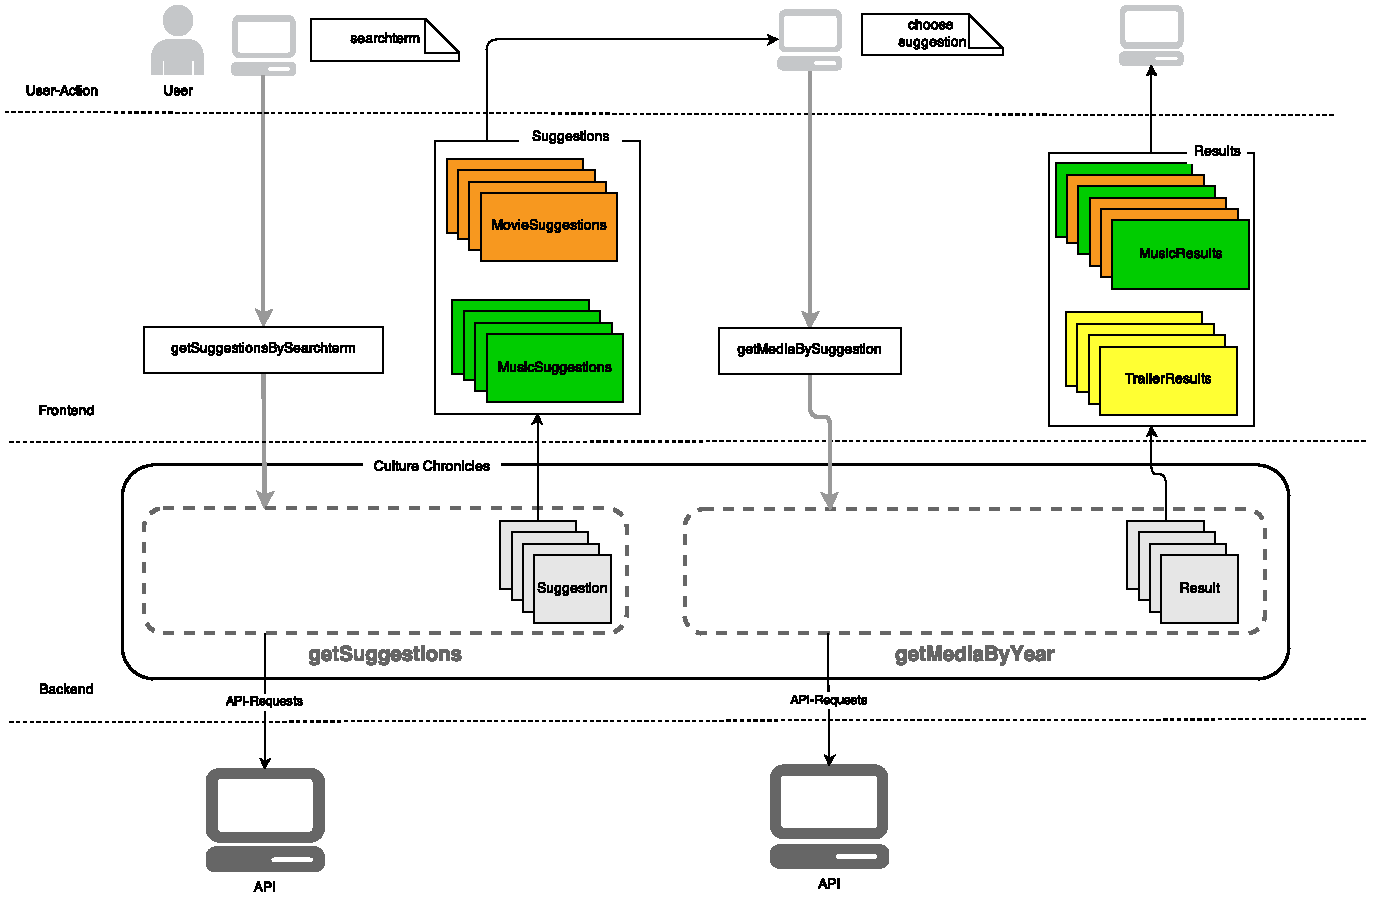
\includegraphics[width=1\textwidth]{Retrieving.pdf}
		\caption{Request-Diagramm}
	\end{center}
	\label{fig:requestDiagram}
\end{figure}

\begin{figure}[htb]
	\begin{center}
		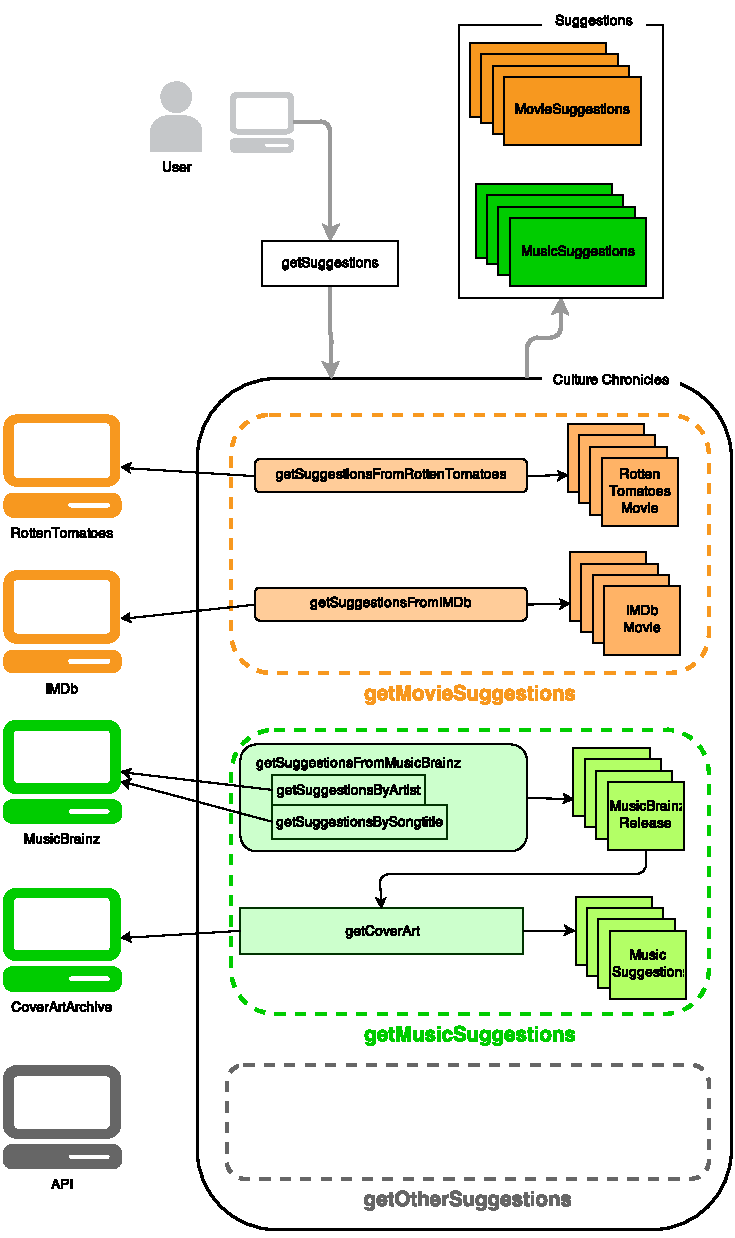
\includegraphics[width=0.7\textwidth]{RetrievingSuggestions.pdf}
		\caption{Suggestions - Request-Diagramm}
	\end{center}
	\label{fig:suggestionsRequestDiagram}
\end{figure}


\begin{figure}[htb]
	\begin{center}
		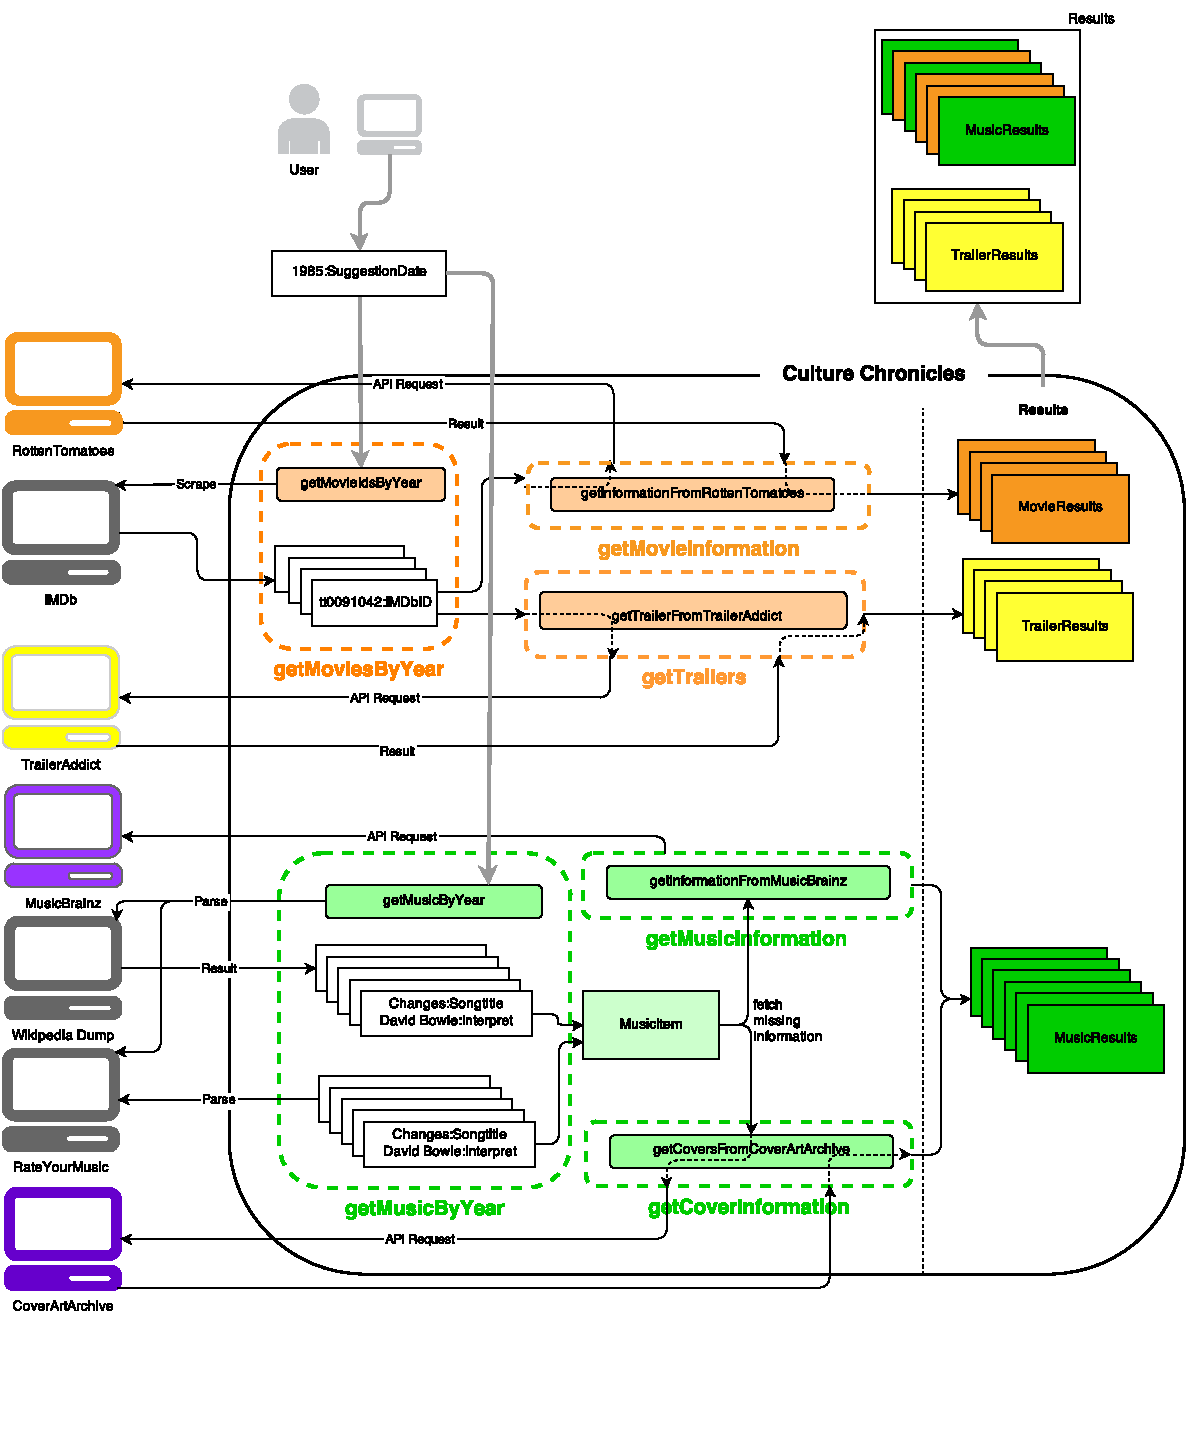
\includegraphics[width=1\textwidth]{RetrievingSearchresultsAndPlaylist.pdf}
		\caption{Searchresults - Request-Diagramm}
	\end{center}
	\label{fig:searchResultsRequestDiagram}
\end{figure}


%\section{Arbeitsweise}


 		%  20-30 Seiten
%     erforderliche/ben�tigte Quellen
%	m�gliche APIs und andere Quellen
%	m�gliche Frameworks f�r die Web-Applikation
%	Grobkonzept
%	Feinkonzept
%	Arbeitsweise
%!TEX root = ../Masterarbeit.tex
\chapter{Ergebnis}
\label{cha:ergebnis}
\begin{itemize}
	\item screenshots vom Prototypen
	\item was ist gut gelaufen, was ist schlecht gelaufen, wo wurde gespart
\end{itemize}				% 3-10 Seiten
%!TEX root = ../Masterarbeit.tex
\chapter{Ausblick}
\label{cha:ausblick}

\section{Problematik und Weiterentwicklung} % Ausblick
\subsection{Abh�ngigkeit von unterschiedlichen APIs}
Im Laufe der Entwicklung von \arbeitstitel \ mussten aufgrund der gro�en Abh�ngigkeit von sehr vielen unterschiedlichen Faktoren sehr viele Kompromisse im Funktionsumfang gemacht werden. Der wichtigste Faktor ist die Verf�gbarkeit der vorhandenen Daten, insbesondere an frei zug�nglichen Musik- oder Film-Charts. �ber Umwege, wie \zB das Web-Scraping, k�nnen zwar auch diese Daten erfasst und verwendet werden, jedoch ist dies zum einen mit erheblichen Mehraufwand verbunden, zum anderen ist dies �u�erst fehleranf�llig. \Va wenn sich Strukturen des Quelltextes �ndern, muss der Code dementsprechend angepasst werden. Au�erdem ist zu Bedenken, dass viele Websites dies ausdr�cklich verbieten. Betreiber von Websites, die diese Technik (noch) nicht ausschlie�en, k�nnen durch erh�hten Traffic, der durch \arbeitstitel \ verursacht w�rde, ebenfalls Urheberrechtsanspr�che geltend machen.

Das Erfassen von Medien-Inhalten ist nicht nur von externen APIs abh�ngig, sondern auch von ihrem Aufbau. Ein Suchbegriff kann einen Songtitel oder einen Interpreten enthalten, d.h., dass f�r die Suche nach einer passenden Musikver�ffentlichung \textbf{MusicBrainz} zwei Requests an die Entit�ten \texttt{Artist} und \texttt{Release-Group} gemacht werden m�ssen. Das Ergebnis ist eine Liste an Release-Groups. Es wird nach Release-Groups gesucht, weil Release-Groups die unterschiedlichen Releases enthalten, die sich gr��tenteils sehr �hneln, da es sich lediglich um unterschiedliche Ver�ffentlichungen in bestimmten L�ndern handelt, w�hrend diese in der Suche von \arbeitstitel \ als ein Medien-Item behandelt werden k�nnen. Eine Suche nach Releases f�hrt also zu sehr vielen redundanten Suchergebnissen. Hinzu kommt, dass die \textbf{Cover Art API} von \textbf{MusicBrainz} ebenfalls eine Release-Group-MusicBrainz-Id ben�tigt. Um jedoch herausfinden zu k�nnen, wann ein Song oder Album ver�ffentlicht wurde, muss anhand der bereits gefundenen Release-Group ein Release gew�hlt werden. Erst anhand einer Release-MusicBrainz-Id kann das Ver�ffentlichungsdatum herausgefunden werden.

SAllein f�r die Abfrage von Suchvorschl�gen von Musik-Ver�ffentlichungen sind diverse Requests an unterschiedliche APIs, \bzw deren Entit�ten, n�tig. Dar�ber hinaus begrenzt \textbf{MusicBrainz} die Anzahl an m�glichen Requests pro Sekunde auf eine Zahl, die f�r das Finden mehrerer Ergebnisse f�r \arbeitstitel \ n�tig sind. Diese Probleme lassen sich allerdings auf unterschiedliche Art und Weise umgehen. Zum einen kann auf die Anzeige eines Album-Covers verzichtet werden. Desweiteren kann, indem die Art der Suchanfrage insofern angepasst wird, dass die Anzahl der erlaubten Requests pro Sekunde nicht �berschritten wird. Dies kann jedoch lediglich als Kompromiss dienen, da dadurch eine gleichzeitige Nutzung durch mehrere Nutzer verhindert w�rde. Eine bessere L�sung ist es, Inhalte in kleineren Bl�cken zu erfassen und jeweils einzelne Datens�tze nachzuladen. Zudem k�nnen zus�tzliche Informationen, die nur zur Anzeige dienen und nicht dem Erfassen des Zeitraumes, nachtr�glich geladen werden, um den Suchprozess selbst nicht unendlich in die L�nge zu ziehen.

Der im Rahmen dieser Master-Arbeit zu implementierende Funktionsumfang der Web-Applikation wurde auf die M�glichkeiten, die das Internet heute bietet, angepasst. Jedoch stellen auch die offizell verwendbaren APIs vor eigene Herausforderungen. Keine der untersuchten APIs bietet eine Suche von Daten-Items anhand eines Zeitpunktes oder Zeitraumes. Dies gilt insbesondere f�r das Erlangen von Informationen �ber Charts. Im Laufe der Implemtierung sind diverse APIs und Techniken untersucht und ausprobiert worden, in welchem Zuge die Behauptung gemacht werden kann, dass eine Einbindung der Medienart Musik sowohl in den Suchvorschl�gen, als auch den Suchergebnissen und im Player, mit den vorher erl�uterten Anpassungen, ohne weitere nennenswerte Probleme eingebunden werden kann.

Zur zweckgem��en Implementierung des Players, muss eines bessere L�sung zur Einbindung abspielbarer Inhalte gefunden werden. Zwar lassen sich Inhalte wie Film-Trailer von \textbf{TrailerAddict} oder Musiktitel �ber die Einbettungs-Funktion von \textbf{Spotify} bereits einbinden, jedoch kann durch das Verwenden von IFrames die Funktionalit�t eines Players nicht gew�hrleistet werden.

F�r die zuk�nftige Weiterentwicklung ist zu sagen, dass mit Projekten wie Wikidata \todo{Semantik und wikidata? oder besser ins fazit?}



\section{Fazit und kritische Bewertung} % Fazit
Ziel dieser Masterarbeit war es, ein umfassendes Konzept einer Web-Appliation zu entwickeln, die das Anzeigen von Inhalten anhand eines gew�hlten Zeitraumes erm�glicht. 
Zum einen um eine Aufarbeitung eines vergangenen Zeitraumes aus nostalgischen Gr�nden, zum anderen die Funktionalit�t zur zeitspezifischen Recherche zu bieten. 
Zu diesem Zweck wurde zun�chst analysiert, inwiefern es bereits M�glichkeiten gibt, Medien-Inhalte anhand eines Zeitpunktes zu suchen. 
Darauf aufbauend ist untersucht worden, inwiefern unterschiedliche Medientypen und -Inhalte relevant f�r eine exemplarische Anzeige eines Zeitraumes sind und welche Medien-Inhalte sich f�r eine Aufbereitung eine repr�sentative �bersicht eignen. 
Es wurde au�erdem ermittelt welche Informationen eines Musikst�ckes, Filmes \oae sich zur Extrahierung eines Zeitpunktes eignen.
Daraus ergab sich eine Sammlung von denkbaren Inhalten, die bei einer zeitspezifischen Recherche von Interesse sein und dargestellt werden k�nnen. 
Im weiteren Verlauf wurde untersucht, inwiefern es m�glich ist, die unterschiedlichen Inhaltstypen wie \zB Musik, Film, Kunst oder News-Artikel, die in einem spefifischen Zeitraum entstanden sind, oder f�r diesen relevant sind, zu erfassen. 
W�hrend es f�r einen Gro�teil der Medienarten diverse Datenquellen, in Form von Web-Diensten, Datenbanken oder sonstigen Schnittstellen, gibt, ergab sich im Laufe der Arbeit der Umstand, dass sich f�r die Mehrheit dieser Daten auf unterschiedliche Arten zwar ein Datum extrahieren l�sst, eine Suche anhand eines Zeitpunktes oder -raumes in den wenigsten F�llen gegeben ist. 
Um eine zeitspezifische Suche anbieten zu k�nnen, sind demnach weitaus mehr Schritte n�tig, als das Abfragen der diversen Datenquellen, die �ber Musik- oder Film-Inhalte verf�gen.  
Den Umst�nden geschuldet, ist im Rahmen der Implementierung		% 3-5 Seiten
% Ausblick
% Fazit





%%!TEX root = ../Masterarbeit.tex
\chapter{Zitate und Referenzen}
\label{cha:ZitateReferenzen}

Die \NeuerBegriff{Service-orientierte Architektur} (SOA) ist seit einiger Zeit \textit{das} Schlagwort im Bereich der Informationstechnologie. So haben \zB Deutschlands gr��te Softwarehersteller SAP und die Software AG ihre Unternehmensstrategie komplett auf die SOA ausgerichtet. \Autor{SAP2007} bietet mit \Fachbegriff{Netweaver} seine marktf�hrende ERP-Software auf Basis von SOA an,\footnote{\Vgl\Zitat[S.~127]{SAP2007}} und die \Autor{Software2007b}, die sich selbst als "`The XML Company"' bezeichnet, erweiterte k�rzlich noch einmal ihr bereits durchg�ngig an der SOA orientiertes Produktportfolio durch den Kauf des amerikanischen Unternehmens webMethods um L�sungen zur Unterst�tzung von Gesch�ftsprozessen.\footnote{\Vgl\Zitat{Software2007b}} In einem Atemzug mit der SOA werden h�ufig Webservices genannt, da sie durch ihre hohe Plattformunabh�ngigkeit und den Einsatz von Internettechnologie oftmals als Referenzimplementierung f�r die Services in einer SOA angef�hrt werden. Doch welche Vorteile bietet der Einsatz von Webservices in Unternehmen? K�nnen mit ihnen tats�chlich flexiblere Softwaresysteme entwickelt werden? Und wie einfach ist die Implementierung von Webservices auf unterschiedlichen Plattformen? Diesen Fragen wird sich der Autor in der vorliegenden Arbeit widmen.

\begin{wrapfigure}{l}{0.5\textwidth}
  \begin{center}
    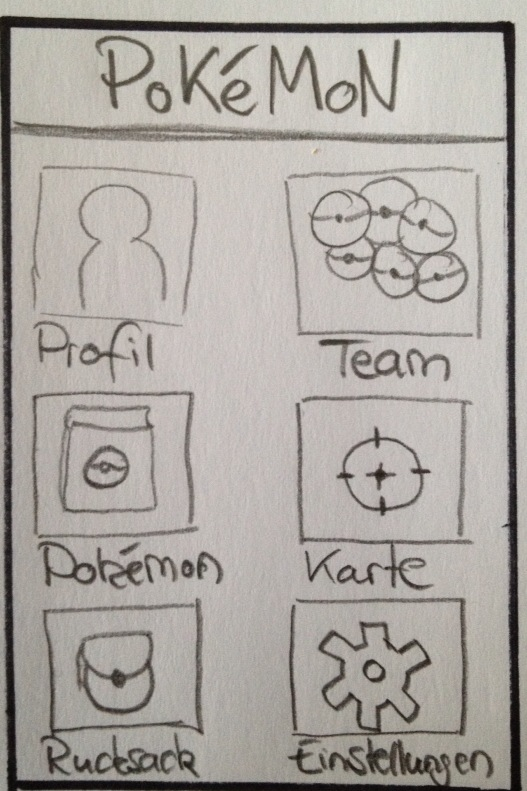
\includegraphics[width=0.48\textwidth]{screens/09_home.jpg}
  \end{center}
  \caption{Home-Screen von dem der Spieler in alle Menu-Punkte navigieren kann.}
\end{wrapfigure}

Wie bereits in Kapitel \ref{cha:Einleitung} auf Seite \pageref{cha:Einleitung} erw�hnt, ist zur Unterst�tzung von Gesch�ftsprozessen der Einsatz von Informationstechnologie notwendig. Der Autor verfolgt mit dieser Arbeit das Ziel, einen Gesch�ftsprozess \todo{Was ist ein Gesch�ftsprozess?} mit Hilfe von Webservices zu optimieren. Hierzu wird er in diesem Kapitel eine Einf�hrung in das Thema Webservices und die damit in Zusammenhang stehenden Technologien geben, und auch auf m�gliche Einsatzbereiche von Webservices im Rahmen der Gesch�ftsprozessoptimierung eingehen. Tabelle \ref{tab:ElementeDerEreignisgesteuertenProzesskette} auf Seite \pageref{tab:ElementeDerEreignisgesteuertenProzesskette} zeigt ganz tolle Sachen.

Ich empfehle allen Softwareentwicklern die Lekt�re von \Zitat{Goodliffe2007}.

\section{Definitionen}
Die Service-orientierte Architektur ist ein Ansatz der Softwareentwicklung, der sich stark am Konzept der Gesch�ftsprozesse orientiert und mit Hilfe von Webservices implementiert werden kann. In den beiden folgenden Kapiteln werden beide Begriffe eingehend erl�utert, worauf in Kapitel \ref{cha:Fazit} die f�r die Umsetzung von Webservices ben�tigten Technologien vorgestellt werden.

\section{Service-orientierte Architektur}
\Autor{OASIS2007}\footnote{Die \NeuerBegriff{Organization for the Advancement of Structured Information Standards} ist nach \Zitat{OASIS2007} ein internationales Konsortium aus �ber 600 Organisationen, das sich der Entwicklung von E-Business-Standards verschrieben hat. Mitglieder sind \zB IBM, SAP und Sun.} definiert den Begriff \NeuerBegriff{Service-orientierte Architektur} (SOA) wie folgt:
\begin{quote}
"`\textbf{Service Oriented Architecture} [\ldots] is a paradigm for organizing and utilizing distributed \textbf{capabilities} that may be under the control of different ownership domains."'\footnote{\Zitat[S.~8]{OASIS2006a}}
\end{quote}
Diese bewusst allgemein gehaltene Definition stammt aus dem Referenzmodell der SOA aus dem Jahr 2006. Dieses Modell wurde mit dem Ziel entwickelt, ein einheitliches Verst�ndnis des Begriffs SOA und des verwendeten Vokabulars zu schaffen, und sollte die zahlreichen bis dato vorhandenen, teils widerspr�chlichen Definitionen abl�sen.\footnote{\Vgl\Zitat[S.~4]{OASIS2006a}} Dabei wird zun�chst noch kein Bezug zur Informationstechnologie hergestellt, sondern allgemein von F�higkeiten gesprochen, die Personen, Unternehmen, aber eben auch Computer besitzen und evtl. Anderen anbieten, um Probleme zu l�sen. Als Beispiel wird ein Energieversorger angef�hrt, der Haushalten seine F�higkeit Strom zu erzeugen anbietet.\footnote{\Vgl\Zitat[S.~8f.]{OASIS2006a}}



\chapter{Bilder und Listings}

In den folgenden drei Kapiteln wird der Autor eine einfache Webservice-Umgebung aufbauen, um zu zeigen, wie Webservices in der Praxis angeboten, konsumiert und orchestriert werden k�nnen. Hierzu verwendet er ausschlie�lich Open-Source-Software, im Speziellen \NeuerBegriff{Apache Tomcat}\footnote{Website: \url{http://tomcat.apache.org/}} als Servlet-Engine, \NeuerBegriff{Apache Axis2}\footnote{Website: \url{http://ws.apache.org/axis2/}} als SOAP-Engine und \NeuerBegriff{ActiveBPEL}\footnote{Website: \url{http://www.activebpel.org/}} als Workflow-System. Die Installation und Konfiguration der ben�tigten Anwendungen wird in Kapitel \ref{sec:Werkzeuge} beschrieben. Die komplette Umgebung inkl. der vom Autor erstellten Webservices befindet sich als virtuelle Maschine auf der dieser Arbeit beigelegten DVD. Im Folgenden wird der DNS-Name \Code{linux-ws} als Bezeichnung f�r den Webservice-Server verwendet.

\section{Anbieten eines Webservice}
\label{sec:AnbietenEinesWebservices}
Mit Hilfe von Apache Axis2 k�nnen Webservices sehr einfach auf Basis von normalen Java-Klassen angeboten werden. Es ist lediglich eine zus�tzliche XML-Datei namens \Datei{META-INF/services.xml} n�tig, in der die zu ver�ffentlichenden Klassen und Methoden beschrieben werden. \abbildung{HelloWorldStruktur} zeigt die Struktur eines einfachen \Webservice{HelloWorld}-Webservice.

\begin{figure}[htb]
\centering
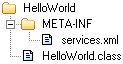
\includegraphics[width=0.3\textwidth]{HelloWorldStruktur.jpg}
\caption{\Webservice{HelloWorld}-Webservice: Dateistruktur}
\label{fig:HelloWorldStruktur}
\end{figure}

Die Klasse \Code{HelloWorld} besitzt nur die Methode \Code{SayHello}, die den \Datentyp{String} \Code{Hello World!} zur�ckgibt. Sie wird in Listing \ref{lst:HelloWorldJava} gezeigt. 

\newpage
\lstset{language=Java, basicstyle=\footnotesize, showstringspaces=false, tabsize=2}
\lstinputlisting[label=lst:HelloWorldJava,caption=\Webservice{HelloWorld}-Webservice: Java-Klasse \Code{HelloWorld}]{DVD/Listings/HelloWorld/HelloWorld.java}

\section{Netzwerkverkehr beim Aufruf von \Webservice{PersonFactory}}

\subsection{SOAP-Request}
Listing \ref{lst:SOAPRequest} zeigt die mitgeschnittene SOAP-Anfrage per HTTP an den Webservice \Webservice{PersonFactory}. Wie am Ende von Kapitel \ref{cha:Einleitung} beschrieben, wird die eigentliche SOAP-Nachricht mittels des HTTP-\Eingabe{POST}-Befehls (Zeile 1) an den Webservice unter der angegebenen URL (Zeile 1) auf dem Server (Zeile 5) geschickt. In Zeile 3 wird �ber den Befehl \Eingabe{SOAPAction} �bermittelt, welche Funktion des Webservice (in diesem Fall \Code{CreatePerson}) aufgerufen werden soll. Die XML-Nutzlast (Zeilen 8--18) besteht dann aus einer einfachen SOAP-Nachricht aus \XMLElement{Envelope}, \XMLElement{Header} und \XMLElement{Body}, die einen RPC durchf�hrt. Die aufzurufenden Funktion wird noch einmal im SOAP-\XMLElement{Body} in Zeile 15 definiert.


\lstset{language=XML, basicstyle=\footnotesize, showstringspaces=false, tabsize=2}
\lstinputlisting[label=lst:SOAPRequest,caption=SOAP-Request an \Webservice{PersonFactory} per HTTP]{DVD/Listings/PersonFactorySOAPRequest.txt}

\subsection{SOAP-Response}
Die Antwort des \Webservice{PersonFactory}-Webservice zeigt Listing \ref{lst:SOAPResponse}. Sie beginnt in Zeile 1 mit dem HTTP-Statuscode 200, der die Anfrage als erfolgreich kennzeichnet. Die eigentliche Nutzlast in Form von XML-Daten (Zeile 3) folgt dann ab Zeile 7. Sie besteht aus dem Element \XMLElement{Person} und seinen Unterelementen, umschlossen vom Element \XMLElement{CreatePersonRepsonse}, das die Antwort-Nachricht aus der WSDL repr�sentiert.

\lstset{language=XML, basicstyle=\footnotesize, showstringspaces=false, tabsize=2}
\lstinputlisting[label=lst:SOAPResponse,caption=SOAP-Response von \Webservice{PersonFactory} per HTTP]{DVD/Listings/PersonFactorySOAPResponse.txt}





\chapter{Aufz�hlungen und Tabellen}


Eine normale Punktliste:
\begin{itemize}
\item Lorem ipsum dolor sit amet, consectetuer adipiscing elit. Nulla ac ipsum a metus viverra tempor. 
\item Nunc sem. Nulla nec urna eu nibh vehicula convallis. Integer ac turpis. Donec mauris enim, dignissim quis, scelerisque ac, rhoncus id, sapien. 
\item Donec turpis felis, cursus in, varius vitae, mollis ac, lorem. Integer a dui sit amet eros nonummy aliquet. Donec egestas adipiscing tellus. Nulla iaculis. 
\item Aliquam erat volutpat. Curabitur posuere, eros vitae accumsan semper, risus erat viverra erat, eu vehicula mi leo at elit. Fusce luctus. Fusce vehicula pretium diam. Nunc sed arcu ut erat suscipit fermentum.
\end{itemize}

Eine nummerierte Liste:
\begin{enumerate}
\item Lorem ipsum dolor sit amet, consectetuer adipiscing elit. Nulla ac ipsum a metus viverra tempor. 
\item Nunc sem. Nulla nec urna eu nibh vehicula convallis. Integer ac turpis. Donec mauris enim, dignissim quis, scelerisque ac, rhoncus id, sapien. 
\item Donec turpis felis, cursus in, varius vitae, mollis ac, lorem. Integer a dui sit amet eros nonummy aliquet. Donec egestas adipiscing tellus. Nulla iaculis. 
\item Aliquam erat volutpat. Curabitur posuere, eros vitae accumsan semper, risus erat viverra erat, eu vehicula mi leo at elit. Fusce luctus. Fusce vehicula pretium diam. Nunc sed arcu ut erat suscipit fermentum.
\end{enumerate}

\begin{enumerate}[a)]
\item Diese Liste...
\item ...hat anstatt der normalen schwarzen Punkte...
\item ...Buchstaben als Marker.
\end{enumerate}


\section{Vom Autor verwendete Software}
\label{sec:Werkzeuge}
Im Folgenden werden die Programme vorgestellt, die der Autor zum Erstellen dieser Arbeit und vor allem zur Entwicklung der Webservices verwendet hat. Soweit es m�glich war, wurden Open-Source-Programme eingesetzt.

\begin{itemize}
\itemd{Microsoft Visio}{Die EPKs der BAP wurden mit Microsoft Visio erstellt. Der Autor hat zwar verschiedene Open-Source-Programme\footnote{Dia, OpenOffice Draw und die EPC Tools.} ausprobiert, mit denen EPKs erstellt werden k�nnten, die grafischen Ergebnisse waren aber nicht zufriedenstellend. Die Symbole von Visio sehen den "`originalen"' ARIS-Symbolen am �hnlichsten und k�nnen dar�ber hinaus mit zus�tzlichen Informationen wie Dauer und Kosten versehen werden.}
\itemd{PSPad}{F�r die Bearbeitung von verschiedenen (Text-)Dateien wurde der Texteditor PSPad verwendet. Mit diesem konnten \zB auch die regul�ren Ausdr�cke f�r die XML-Schemas entwickelt werden. Website: \url{http://www.pspad.com/}}
\itemd{Eclipse}{Sowohl der ActiveBPEL Designer als auch die EntireX Workbench sind Plugins f�r die IDE Eclipse. Auch zur Java- und PHP-Entwicklung wurde dieses Werkzeug verwendet. Website: \url{http://www.eclipse.org/}}
\itemd{XML Copy Editor}{F�r die Entwicklung der XML-Schemas und die Bearbeitung von XML-Dateien wurde der XML Copy Editor eingesetzt. Mit diesem k�nnen \ua XML-Dateien auf Wohlgeformtheit gepr�ft und gegen ihr Schema validiert werden. Website: \url{http://xml-copy-editor.sourceforge.net/}}
\itemd{soapUI}{
Mit soapUI k�nnen Webservices getestet werden, ohne einen Client zu programmieren. Die SOAP-Anfragen werden automatisch anhand der WSDL generiert und die Antworten k�nnen gegen die WSDL-Datei validiert werden. Website: \url{http://www.soapui.org/}}
\itemd{Ethereal}{
Die Netzwerkkommunikation beim Aufrufen der Webservices wurde mit Ethereal, einem umfangreichen Werkzeug zur Analyse des Netzwerkverkehrs, mitgeschnitten. Website: \url{http://www.ethereal.com/}}
\itemd{\LaTeX}{
Diese Arbeit wurde mit {\LaTeX} geschrieben. Als Distribution wurde MiKTeX verwendet und als Editor der LaTeX Editor. Websites: \url{http://miktex.org/}, \url{http://www.latexeditor.org/}}
\end{itemize}

\section{Elemente der Ereignisgesteuerten Prozesskette}

\begin{longtable}{|m{10cm}|m{3cm}|}
\caption{Elemente der Ereignisgesteuerten Prozesskette} \\
\hline
\label{tab:ElementeDerEreignisgesteuertenProzesskette}
\textbf{Element} & \textbf{Symbol}\\
\hline
\textbf{Funktion} 

Funktionen beschreiben T�tigkeiten, die im Verlauf des Gesch�ftsprozesses anfallen. Sie k�nnen von Mitarbeitern oder einem Informationssystem durchgef�hrt werden und ben�tigen evtl. Ressourcen, die ihnen zugewiesen werden. 

Beispiele: \textit{Auftrag anlegen}, \textit{Rechnung schreiben}, \textit{Konto abschlie�en} & 
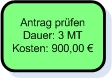
\includegraphics[width=3cm]{EPK-Funktion.jpg} \\
\hline
\textbf{Ereignis} 

Ereignisse sind betriebswirtschaftlich relevante Ereignisse, die den Gesch�ftsprozess in irgendeiner Weise steuern oder beeinflussen. Ereignisse sind immer Ausl�ser oder Ergebnisse von Funktionen. Ein Gesch�ftsprozess beginnt und endet stets mit einem Ereignis. 

Beispiele: \textit{Auftrag eingetroffen}, \textit{�berweisung get�tigt}, \textit{Rechnung erstellt} & 
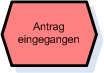
\includegraphics[width=3cm]{EPK-Ereignis.jpg} \\
\hline
\textbf{Operatoren} 

Operatoren steuern den Kontrollfluss eines Gesch�ftsprozesses. Sie machen \zB deutlich, dass eine Funktion mehrere Ereignisse ausl�st, oder zeigen alternative Vorgehensweisen an. Es gibt drei Operatoren (v.\,l.\,n.\,r.\,): UND, ODER und XODER (exklusives ODER). & 

\includegraphics[width=3cm]{EPK-Operatoren.jpg} \\
\hline
\textbf{Organisationseinheit} 

Organisationseinheiten werden Funktionen zugeordnet und beschreiben, wo die Funktionen ausgef�hrt werden bzw. wer sie ausf�hrt. Die Bezeichnung der Symbole enth�lt zus�tzlich zur Abteilung noch die Namen der Mitarbeiter.

Beispiele: \textit{Vertrieb}, \textit{Personal}, \textit{Produktion} & 
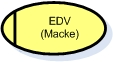
\includegraphics[width=3cm]{EPK-Organisationseinheit.jpg} \\
\hline
\textbf{Informationsobjekt} 

Auch Informationsobjekte werden Funktionen zugewiesen und beschreiben die von diesen ben�tigten oder erstellten Informationen. Dabei sind s�mtliche Formen von Informationen auf verschiedenen Datentr�gern m�glich und nicht etwa nur digitale Daten. Die Bezeichnung der Symbole enth�lt zus�tzlich das Informationssystem, aus dem die Informationen stammen.

Beispiele: \textit{Kundendatenbank}, \textit{Versicherungsantrag}, \textit{Rechnung} & 
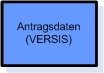
\includegraphics[width=3cm]{EPK-Informationen.jpg} \\
\hline
\textbf{Prozesswegweiser}

Mit Prozesswegweisern werden Prozesse, die in anderen EPKs beschrieben sind, referenziert. So k�nnen \zB un�bersichtliche Prozesse in Teilprozesse gegliedert und h�ufig verwendete Prozesse an zentraler Stelle modelliert werden. Prozesswegweiser stehen in einer EPK immer anstelle von Funktionen. & 
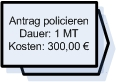
\includegraphics[width=3cm]{EPK-Prozesspfad.jpg} \\
\hline
\end{longtable}

% Literaturverzeichnis ---------------------------------------------------------
%   Das Literaturverzeichnis wird aus der BibTeX-Datenbank "Bibliographie.bib"
%   erstellt.
% ------------------------------------------------------------------------------
\bibliography{MasterBibliographie} % Aufruf: bibtex Masterarbeit
%\bibliographystyle{natdin} % DIN-Stil des Literaturverzeichnisses
\bibliographystyle{jurabib}

\addchap{Eidesstattliche Erkl�rung}
Ich, \autor, Matrikel-Nr.\ \matrikelnr, versichere hiermit, dass ich meine Masterarbeit mit dem Thema
\begin{quote}
\textit{\titel} \textit{\untertitel}
\end{quote}
selbst�ndig verfasst und keine anderen als die angegebenen Quellen und Hilfsmittel benutzt habe, wobei ich alle w�rtlichen und sinngem��en Zitate als solche gekennzeichnet habe. Die Arbeit wurde bisher keiner anderen Pr�fungsbeh�rde vorgelegt und auch nicht ver�ffentlicht.

Mir ist bekannt, dass ich meine Masterarbeit zusammen mit dieser Erkl�rung fristgem�� nach Vergabe des Themas in dreifacher Ausfertigung und gebunden im Pr�fungsamt der \hochschule \ abzugeben oder sp�testens mit dem Poststempel des Tages, an dem die Frist abl�uft, zu senden habe.\\[6ex]

\ort, den \today


\rule[-0.2cm]{5cm}{0.5pt}

\textsc{\autor} 
 % Selbst�ndigkeitserkl�rung

% Anhang -----------------------------------------------------------------------
%   Die Inhalte des Anhangs werden analog zu den Kapiteln inkludiert.
%   Dies geschieht in der Datei "Anhang.tex".
% ------------------------------------------------------------------------------
\begin{appendix}
   \clearpage
   \pagenumbering{roman}
   \chapter{Anhang}
   \label{sec:Anhang}
   % Rand der Aufz�hlungen in Tabellen anpassen
   \setdefaultleftmargin{1em}{}{}{}{}{}
   %!TEX root = Masterarbeit.tex
\label{app:matrix}
\begin{landscape}
	%!TEX root = ../../Masterarbeit.tex
\begin{landscape}
\begin{longtable}{ll>{\raggedright}p{0.75\textwidth}l>{\raggedright}p{0.75\textwidth}lll}
    Film                  & ~                                                               & ~                                                                                         & ~                                                                                                                                                                                                                          & ~                                           & ~                                                                  \\
    ~                     & ~                                                               & ~                                                                                         & ~                                                                                                                                                                                                                          & ~                                           & ~                                                                  \\
    Zeitraum              & Suchbegriff                                                     & Link zum Suchergebnis                                                                     & �berschrift                                                                                                                                                                                                                & Beschreibung                                & Bewertung                                                          \\
    google.de             & ~                                                               & ~                                                                                         & ~                                                                                                                                                                                                                          & ~                                           & ~                                                                  \\
    Achtziger             & \glqq movies 80s\grqq                                                     & \url{http://www.digitaldreamdoor.com/pages/movie-pages/movie\_80s.html}                         & 100 Greatest Movies of the 1980s                                                                                                                                                                                           & Top 100                                     & \textasteriskcentered \textasteriskcentered      \\
    ~                     & ~                                                               & \url{http://en.wikipedia.org/wiki/1980s\_in\_film}                                              & 1980s in film                                                                                                                                                                                                              & Filmgeschichtlicher Artikel                 & \textasteriskcentered \textasteriskcentered      \\
    ~                     & ~                                                               & \url{http://www.imdb.com/search/title/?release\_date=1980,1989\&title\_type=feature}            & Most Popular Feature Films Released 1980 to 1989                                                                                                                                                                           & Top 50                                      & \textasteriskcentered \textasteriskcentered \textasteriskcentered  \\
    Neunziger             & \glqq movies 90s\grqq                                                    & \url{http://www.digitaldreamdoor.com/pages/movie-pages/movie\_90s.html}                         & 100 Greatest Movies of the 1990s                                                                                                                                                                                           & Top 100                                     & \textasteriskcentered \textasteriskcentered      \\
    ~                     & ~                                                               & \url{http://www.pinterest.com/richhadbroo/100-great-90-s-movies/}                               & 100 great 90's movies                                                                                                                                                                                                      & Pinterest Top 100 mit Filmplakaten          & ~                                                                  \\
    ~                     & ~                                                               & \url{http://www.pinterest.com/roxsan13/best-90s-movies/}                                        & best 90s movies                                                                                                                                                                                                            & Pinterest Liste mit Filmplakaten            & ~                                                                  \\
    Vietnamkrieg          & \glqq movies vietnam war\grqq                                            & \url{http://en.wikipedia.org/wiki/Category:Vietnam\_War\_films}                                 & Category:Vietnam War films                                                                                                                                                                                                 & Alphabetische Liste von Filmen              & \textasteriskcentered \textasteriskcentered      \\
    ~                     & ~                                                               & \url{http://en.wikipedia.org/wiki/Vietnam\_War\_in\_film}                                       & Vietnam War in film                                                                                                                                                                                                        & Liste von Filmen mit dem Thema Vietnamkrieg & \textasteriskcentered \textasteriskcentered      \\
    ~                     & ~                                                               & \url{http://warmovies.about.com/od/TopPicks/tp/Top-10-Vietnam-Films-Of-All-Time.htm}            & Top 10 Vietnam Films of All Time                                                                                                                                                                                           & Subjektive Top Ten Liste                    & \textasteriskcentered                                     \\
    ~                     & ~                                                               & ~                                                                                         & ~                                                                                                                                                                                                                          & ~                                           & ~                                                                  \\
    en.wikipedia.org      & ~                                                               & ~                                                                                         & ~                                                                                                                                                                                                                          & ~                                           & ~                                                                  \\
    Achtziger             & \glqq movie 80s\grqq                                                     & \url{http://en.wikipedia.org/wiki/1980s\_in\_film}                                              & 1980s in film                                                                                                                                                                                                              & Filmgeschichtlicher Artikel                 & \textasteriskcentered \textasteriskcentered      \\
    ~                     & ~                                                               & \url{http://en.wikipedia.org/wiki/Alan\_Hunter\_(VJ)}                                           & Alan Hunter (VJ)                                                                                                                                                                                                           & VJ-Seite                                    & ~                                                                  \\
    ~                     & ~                                                               & \url{http://en.wikipedia.org/wiki/American\_Top\_40}                                            & American Top 40                                                                                                                                                                                                            & Musik-Top 40                                & ~                                                                  \\
    Neunziger             & \glqq movie 90s\grqq                                                     & \url{http://en.wikipedia.org/wiki/TeenNick}                                                     & TeenNick                                                                                                                                                                                                                   & TV Sender                                   & ~                                                                  \\
    ~                     & ~                                                               & \url{http://en.wikipedia.org/wiki/R.\_Kelly}                                                    & R. Kelly                                                                                                                                                                                                                   & Musikerseite                                & ~                                                                  \\
    ~                     & ~                                                               & \url{http://en.wikipedia.org/wiki/Ace\_of\_Base}                                                & Ace Of Base                                                                                                                                                                                                                & Bandseite                                   & ~                                                                  \\
    Vietnamkrieg          & \glqq vietnam war music\grqq                                             & \url{http://en.wikipedia.org/wiki/Vietnam\_War\_in\_film}                                       & Vietnam War in film                                                                                                                                                                                                        & Liste von Filmen mit dem Thema Vietnamkrieg & \textasteriskcentered \textasteriskcentered      \\
    ~                     & ~                                                               & \url{http://en.wikipedia.org/wiki/Vietnam\_War}                                                 & Vietnam War                                                                                                                                                                                                                & Artikel �ber den Vietnamkrieg               & ~                                                                  \\
    ~                     & ~                                                               & \url{http://en.wikipedia.org/wiki/Apocalypse\_Now}                                              & Apocalypse Now                                                                                                                                                                                                             & Filmseite                                   & \textasteriskcentered                                     \\
    ~                     & ~                                                               & ~                                                                                         & ~                                                                                                                                                                                                                          & ~                                           & ~                                                                  \\
    Amazon.com            & ~                                                               & ~                                                                                         & ~                                                                                                                                                                                                                          & ~                                           & ~                                                                  \\
    Achtziger             & \glqq 80s\grqq  mit Filter \glqq Movies \& TV\grqq                                 & \url{http://www.amazon.com/Spotlight-Collection-Breakfast-Universals-Anniversary/dp/B006TTC50Y} & 80s Comedies Spotlight Collection [The Breakfast Club, Sixteen Candles, Fast Times at Ridgemont High] (Universal's 100th Anniversary) (1982)                                                                               & Filmsammlung                                & \textasteriskcentered \textasteriskcentered      \\
    ~                     & ~                                                               & \url{http://www.amazon.com/Pure-80s-Ultimate-DVD-Region/dp/B000FUTUY2}                          & Pure '80s: The Ultimate DVD Box [Region 1] (2006)                                                                                                                                                                          & Filmsammlung                                & \textasteriskcentered                                     \\
    ~                     & ~                                                               & \url{http://www.amazon.com/Excellent-Eighties-Demi-Moore/dp/B008L0YN0Y}                         & Excellent Eighties (1980)                                                                                                                                                                                                  & Filmsammlung                                & \textasteriskcentered                                     \\
    Neunziger             & \glqq 90s\grqq mit Filter \glqq Movies \& TV\grqq                                 & \url{http://www.amazon.com/WWE-Greatest-Stars-90s-Rock/dp/B001PPLJOU}                           & WWE: Greatest Stars of the '90s (2009)                                                                                                                                                                                     & DVD-Box der gr��ten Stars der 80er          & ~                                                                  \\
    ~                     & ~                                                               & \url{http://www.amazon.com/Costello-Society-Naughty-Nineties-Privates/dp/B0001FGBZM}            & The Best of Abbott \& Costello, Vol. 2 (Hit the Ice / In Society / Here Come the Co-Eds / The Naughty Nineties / Little Giant / The Time of Their Lives / Buck Privates Come Home / The Wistful Widow of Wagon Gap) (1943) & Filmsammlung �ber Abbott und Castello       & \textasteriskcentered                                     \\
    ~                     & ~                                                               & \url{http://www.amazon.com/90s-Night-8-Movie-Will-Ferrell/dp/B00GOC74WA}                        & 90s Night In - 8-Movie Set                                                                                                                                                                                                 & Filmsammlung                                & \textasteriskcentered \textasteriskcentered      \\
    Vietnamkrieg          & \glqq vietnam war\grqq mit Filter \glqq Movies \& TV\grqq                         & \url{http://www.amazon.com/Vietnam-War-Tour-Duty-Patrol/dp/B004P1DWYG}                          & The Vietnam War Tour of Duty on Patrol                                                                                                                                                                                     & Dokumentation                               & \textasteriskcentered                                     \\
    ~                     & ~                                                               & \url{http://www.amazon.com/gp/product/B0064YPMYK}                                               & Vietnam in HD Season 1, Ep. 1 \glqq The Beginning (1964-1965)\grqq                                                                                                                                                                  & Dokumentation                               & \textasteriskcentered                                     \\
    ~                     & ~                                                               & \url{http://www.amazon.com/Vietnam-Ten-Thousand-Day-War/dp/B00ARWXJ54}                          & Vietnam: The Ten Thousand Day War                                                                                                                                                                                          & Film                                        & \textasteriskcentered                                     \\
    ~                     & ~                                                               & ~                                                                                         & ~                                                                                                                                                                                                                          & ~                                           & ~                                                                  \\
    imdb.com              & ~                                                               & ~                                                                                         & ~                                                                                                                                                                                                                          & ~                                           & ~                                                                  \\
    Achtziger             & \glqq 80s\grqq                                                           & \url{http://www.imdb.com/title/tt0480953/}                                                      & 80s (2005- )                                                                                                                                                                                                               & TV-Serie                                    & ~                                                                  \\
    ~                     & ~                                                               & \url{http://www.imdb.com/title/tt2805998}                                                       & Talk Stoop with Cat Greenleaf                                                                                                                                                                                              & TV-Serie                                    & ~                                                                  \\
    ~                     & ~                                                               & \url{http://www.imdb.com/title/tt0305472}                                                       & That \grq 80s Show (2002- )                                                                                                                                                                                                    & TV-Serie                                    & ~                                                                  \\
    Neunziger             & \glqq 90s\grqq                                                           & \url{http://www.imdb.com/title/tt0415430}                                                       & I Love the \grq 90s (2004- )                                                                                                                                                                                                   & TV-Serie                                    & ~                                                                  \\
    ~                     & ~                                                               & \url{http://www.imdb.com/title/tt3223572}                                                       & The Big Fat Quiz of the 90s (2013)                                                                                                                                                                                         & TV-Movie                                    & \textasteriskcentered                                     \\
    ~                     & ~                                                               & \url{http://www.imdb.com/title/tt1003289}                                                       & Saturday Night Live in the '90s: Pop Culture Nation (2007)                                                                                                                                                                 & TV-Movie                                    & \textasteriskcentered                                     \\
    Vietnamkrieg          & \glqq vietnam war\grqq                                                   & \url{http://www.imdb.com/title/tt0793563}                                                       & Vietnam War (2002)                                                                                                                                                                                                         & Video Game                                  & ~                                                                  \\
    ~                     & ~                                                               & \url{http://www.imdb.com/title/tt0098597}                                                       & Vietnam War Story: The Last Days                                                                                                                                                                                           & Dokumentation                               & ~                                                                  \\
    ~                     & ~                                                               & \url{http://www.imdb.com/title/tt0092475}                                                       & Vietnam War Story (1987-1988)                                                                                                                                                                                              & TV-Serie                                    & ~                                                                  \\
    ~                     & ~                                                               & ~                                                                                         & ~                                                                                                                                                                                                                          & ~                                           & ~                                                                  \\
    imdb.com/search/title & ~                                                               & ~                                                                                         & ~                                                                                                                                                                                                                          & ~                                           & ~                                                                  \\
    Achtziger             & Release Date: 1980-1989\\Title Type: \\Feature Film, TV Movie\\ & \url{http://www.imdb.com/title/tt0093870}                                                       & RoboCop (1987)                                                                                                                                                                                                             & Film                                        & \textasteriskcentered \textasteriskcentered \textasteriskcentered  \\
    ~                     & ~                                                               & \url{http://www.imdb.com/title/tt0093779}                                                       & Die Braut des Prinzen (1987)                                                                                                                                                                                               & Film                                        & \textasteriskcentered \textasteriskcentered \textasteriskcentered  \\
    ~                     & ~                                                               & \url{http://www.imdb.com/title/tt0081505}                                                       & Shining (1980)                                                                                                                                                                                                             & Film                                        & \textasteriskcentered \textasteriskcentered \textasteriskcentered  \\
    Neunziger             & Release Date: 1990-1999\\Title Type: \\Feature Film, TV Movie\\ & \url{http://www.imdb.com/title/tt0111161}                                                       & Die Verurteilten (1994)                                                                                                                                                                                                    & Film                                        & \textasteriskcentered \textasteriskcentered \textasteriskcentered  \\
    ~                     & ~                                                               & \url{http://www.imdb.com/title/tt0120338}                                                       & Titanic (1997)                                                                                                                                                                                                             & Film                                        & \textasteriskcentered \textasteriskcentered \textasteriskcentered  \\
    ~                     & ~                                                               & \url{http://www.imdb.com/title/tt0137523}                                                       & Fight Club (1999)                                                                                                                                                                                                          & Film                                        & \textasteriskcentered \textasteriskcentered \textasteriskcentered  \\
\end{longtable}
\end{landscape}
% Relevanz
% Qualit�t
% automatische Auswertbarkeit
\end{landscape}

\end{appendix}

% Index ------------------------------------------------------------------------
%   Zum Erstellen eines Index, die folgende Zeile auskommentieren.
% ------------------------------------------------------------------------------
%\printindex

\end{document}
